%%%%% Set up %%%%%

% Set document style and font size
\documentclass[12pt]{article}\usepackage[]{graphicx}\usepackage[]{color}
%% maxwidth is the original width if it is less than linewidth
%% otherwise use linewidth (to make sure the graphics do not exceed the margin)
\makeatletter
\def\maxwidth{ %
  \ifdim\Gin@nat@width>\linewidth
    \linewidth
  \else
    \Gin@nat@width
  \fi
}
\makeatother

\definecolor{fgcolor}{rgb}{0.345, 0.345, 0.345}
\newcommand{\hlnum}[1]{\textcolor[rgb]{0.686,0.059,0.569}{#1}}%
\newcommand{\hlstr}[1]{\textcolor[rgb]{0.192,0.494,0.8}{#1}}%
\newcommand{\hlcom}[1]{\textcolor[rgb]{0.678,0.584,0.686}{\textit{#1}}}%
\newcommand{\hlopt}[1]{\textcolor[rgb]{0,0,0}{#1}}%
\newcommand{\hlstd}[1]{\textcolor[rgb]{0.345,0.345,0.345}{#1}}%
\newcommand{\hlkwa}[1]{\textcolor[rgb]{0.161,0.373,0.58}{\textbf{#1}}}%
\newcommand{\hlkwb}[1]{\textcolor[rgb]{0.69,0.353,0.396}{#1}}%
\newcommand{\hlkwc}[1]{\textcolor[rgb]{0.333,0.667,0.333}{#1}}%
\newcommand{\hlkwd}[1]{\textcolor[rgb]{0.737,0.353,0.396}{\textbf{#1}}}%
\let\hlipl\hlkwb

\usepackage{framed}
\makeatletter
\newenvironment{kframe}{%
 \def\at@end@of@kframe{}%
 \ifinner\ifhmode%
  \def\at@end@of@kframe{\end{minipage}}%
  \begin{minipage}{\columnwidth}%
 \fi\fi%
 \def\FrameCommand##1{\hskip\@totalleftmargin \hskip-\fboxsep
 \colorbox{shadecolor}{##1}\hskip-\fboxsep
     % There is no \\@totalrightmargin, so:
     \hskip-\linewidth \hskip-\@totalleftmargin \hskip\columnwidth}%
 \MakeFramed {\advance\hsize-\width
   \@totalleftmargin\z@ \linewidth\hsize
   \@setminipage}}%
 {\par\unskip\endMakeFramed%
 \at@end@of@kframe}
\makeatother

\definecolor{shadecolor}{rgb}{.97, .97, .97}
\definecolor{messagecolor}{rgb}{0, 0, 0}
\definecolor{warningcolor}{rgb}{1, 0, 1}
\definecolor{errorcolor}{rgb}{1, 0, 0}
\newenvironment{knitrout}{}{} % an empty environment to be redefined in TeX

\usepackage{alltt}

% File path to resources (style file etc)
\newcommand{\locRepo}{csas-style}

% Style file for DFO Technical Reports
\usepackage{\locRepo/tech-report}

% header-includes from R markdown entry
\usepackage{float}

%%%%% Variables %%%%%

% New definitions: Title, year, report number, authors
% Protect lower case words (i.e., species names) in \Addlcwords{}, in "TechReport.sty"
\newcommand{\trTitle}{Summary of the annual 2022 Sablefish (\emph{Anoplopoma fimbria}) trap survey, October - November , 2022}
\newcommand{\trYear}{2023}
\newcommand{\trReportNum}{nnn}
% Optional
\newcommand{\trAuthFootA}{Email: \link{mailto:Lisa.Lacko@dfo-mpo.gc.ca}{\nolinkurl{Lisa.Lacko@dfo-mpo.gc.ca}} \textbar{} telephone: (778) 268-3236}
\newcommand{\trAuthsLong}{Schon M. Acheson, Lisa C. Lacko and Kendra R. Holt}
\newcommand{\trAuthsBack}{Acheson, S.M., Lacko, L.C. and Holt, K.R.}

% New definition: Address
\newcommand{\trAddy}{\textsuperscript{1}Pacific Biological Station\\
Fisheries and Oceans Canada, 3190 Hammond Bay Road\\
Nanaimo, British Columbia, V9T 6N7, Canada\\}

% Abstract
\newcommand{\trAbstract}{This document describes sampling activities and summarizes results from the 2022 British Columbia Sablefish research and assessment survey. The survey was comprised of stratified random sets (StRS) at five depth-stratified areas and standardized sets at one traditional inlet locality. Four sets were dedicated to bottom contact research with 3 deep-water autonomous cameras mounted on a 60 trap string. Biological sampling was conducted for Sablefish and incidentally captured species such as rockfishes and Lingcod. Sablefish were randomly sampled from every third trap on all sets, up to a maximum sample count of 50. The tag and release study conducted annually since 1991 was continued in 2022.

A total of Sablefish were caught on StRS sets in 2022, of which were used for biological samples and were tagged and released. Due to weather conditions, out of 111 planned StRS blocks and one out of four mainland inlets were surveyed. Survey CPUE are presented in relation to previous years to describe trends over time. The 2022 Stratified Random Survey (StRS) is up 10\% from 2021; second highest index since 2003.}

% Resume (i.e., French abstract)
\newcommand{\trResume}{Voici le résumé. Lorem ipsum dolor sit amet, consectetur adipisicing elit, sed do eiusmod tempor incididunt ut labore et dolore magna aliqua. Ut enim ad minim veniam, quis nostrud exercitation ullamco laboris nisi ut aliquip ex ea commodo consequat. Duis aute irure dolor in reprehenderit in voluptate velit esse cillum dolore eu fugiat nulla pariatur. Excepteur sint occaecat cupidatat non proident, sunt in culpa qui officia deserunt mollit anim id est laborum.}

\newcommand{\trISBN}{}

\DeclareGraphicsExtensions{.png,.pdf}
%%%%% Start %%%%%

% Start the document
\IfFileExists{upquote.sty}{\usepackage{upquote}}{}

% commands and environments needed by pandoc snippets
% extracted from the output of `pandoc -s`
%% Make R markdown code chunks work
\usepackage{array}
\usepackage{amssymb,amsmath}
\usepackage{color}
\usepackage{fancyvrb}

% From default template:
\newcommand{\VerbBar}{|}
\newcommand{\VERB}{\Verb[commandchars=\\\{\}]}
\DefineVerbatimEnvironment{Highlighting}{Verbatim}{commandchars=\\\{\},formatcom=\color[rgb]{0.00,0.00,0.00}}
\usepackage{framed}
\definecolor{shadecolor}{RGB}{248,248,248}
\newenvironment{Shaded}{\begin{snugshade}}{\end{snugshade}}
\newcommand{\AlertTok}[1]{\textcolor[rgb]{0.94,0.16,0.16}{#1}}
\newcommand{\AnnotationTok}[1]{\textcolor[rgb]{0.56,0.35,0.01}{\textbf{\textit{#1}}}}
\newcommand{\AttributeTok}[1]{\textcolor[rgb]{0.77,0.63,0.00}{#1}}
\newcommand{\BaseNTok}[1]{\textcolor[rgb]{0.00,0.00,0.81}{#1}}
\newcommand{\BuiltInTok}[1]{#1}
\newcommand{\CharTok}[1]{\textcolor[rgb]{0.31,0.60,0.02}{#1}}
\newcommand{\CommentTok}[1]{\textcolor[rgb]{0.56,0.35,0.01}{\textbf{#1}}}
\newcommand{\CommentVarTok}[1]{\textcolor[rgb]{0.56,0.35,0.01}{\textbf{\textit{#1}}}}
\newcommand{\ConstantTok}[1]{\textcolor[rgb]{0.00,0.00,0.00}{#1}}
\newcommand{\ControlFlowTok}[1]{\textcolor[rgb]{0.13,0.29,0.53}{\textit{#1}}}
\newcommand{\DataTypeTok}[1]{\textcolor[rgb]{0.13,0.29,0.53}{#1}}
\newcommand{\DecValTok}[1]{\textcolor[rgb]{0.00,0.00,0.81}{#1}}
\newcommand{\DocumentationTok}[1]{\textcolor[rgb]{0.56,0.35,0.01}{\textbf{\textit{#1}}}}
\newcommand{\ErrorTok}[1]{\textcolor[rgb]{0.64,0.00,0.00}{\textit{#1}}}
\newcommand{\ExtensionTok}[1]{#1}
\newcommand{\FloatTok}[1]{\textcolor[rgb]{0.00,0.00,0.81}{#1}}
\newcommand{\FunctionTok}[1]{\textcolor[rgb]{0.00,0.00,0.00}{#1}}
\newcommand{\ImportTok}[1]{#1}
\newcommand{\InformationTok}[1]{\textcolor[rgb]{0.56,0.35,0.01}{\textbf{\textit{#1}}}}
\newcommand{\KeywordTok}[1]{\textcolor[rgb]{0.13,0.29,0.53}{\textit{#1}}}
\newcommand{\NormalTok}[1]{#1}
\newcommand{\OperatorTok}[1]{\textcolor[rgb]{0.81,0.36,0.00}{\textit{#1}}}
\newcommand{\OtherTok}[1]{\textcolor[rgb]{0.56,0.35,0.01}{#1}}
\newcommand{\PreprocessorTok}[1]{\textcolor[rgb]{0.56,0.35,0.01}{\textbf{#1}}}
\newcommand{\RegionMarkerTok}[1]{#1}
\newcommand{\SpecialCharTok}[1]{\textcolor[rgb]{0.00,0.00,0.00}{#1}}
\newcommand{\SpecialStringTok}[1]{\textcolor[rgb]{0.31,0.60,0.02}{#1}}
\newcommand{\StringTok}[1]{\textcolor[rgb]{0.31,0.60,0.02}{#1}}
\newcommand{\VariableTok}[1]{\textcolor[rgb]{0.00,0.00,0.00}{#1}}
\newcommand{\VerbatimStringTok}[1]{\textcolor[rgb]{0.31,0.60,0.02}{#1}}
\newcommand{\WarningTok}[1]{\textcolor[rgb]{0.56,0.35,0.01}{\textbf{\textit{#1}}}}
\begin{document}

%%%% Front matter %%%%%

% Add the first few pages
\frontmatter

%%%%% Drafts %%%%%

%\linenumbers  % Line numbers
%\onehalfspacing  % Extra space between lines
\renewcommand{\headrulewidth}{0.5pt}  % Header line
\renewcommand{\footrulewidth}{0.5pt}  % footer line
%\pagestyle{fancy}\fancyhead[c]{Draft: Do not cite or circulate}  % Header text

\newcommand{\lt}{\ensuremath <}
\newcommand{\gt}{\ensuremath >}

%Defines cslreferences environment
%Required by pandoc 2.8
%Copied from https://github.com/rstudio/rmarkdown/issues/1649
\newlength{\cslhangindent}
\setlength{\cslhangindent}{1.5em}
\newenvironment{cslreferences}%
  {}%
  {\par}

%%%%% Main document %%%%%
\hypertarget{sec:introduction}{%
\section{Introduction}\label{sec:introduction}}

Fishery-independent research surveys using longline trap gear have been conducted by the Department of Fisheries and Oceans (DFO) in collaboration with the Canadian Sablefish Association under a collaborative agreement. Survey procedures have evolved over the years with 1. standardized fishing sets (1988 - 2010) and traditional tagging sets (1991 - 2007) conducted at offshore indexing localities; 2. traditional tagging sets conducted at offshore tagging localities (1995 - 2008); 3. standardized fishing sets conducted at mainland inlet localities (1994 - 2019, 2021, 2022); and 4. stratified random sets conducted within five spatial strata (2003-2022).

The stratified random survey is used to obtain catch rate data, gather biological samples, capture oceanographic measurements, record gear bottom contact and collect tag release and recapture data. This information is used as the key contemporary index of abundance for assessing the biological status of the Sablefish stock, and to condition an operating model that serves as the biological basis of the coastal Management Strategy Evaluation (\protect\hyperlink{ref-DFO2020}{DFO 2020}). In 2021 and 2022, the Canadian Sablefish Association supported a multi-year research study with camera equipment to understand and quantify movement of longline trap gear.

\clearpage

\hypertarget{methods}{%
\section{Methods}\label{methods}}

\hypertarget{survey-design}{%
\subsection{SURVEY DESIGN}\label{survey-design}}

Methodology for the 2022 Sablefish research and assessment surveys employed a stratified random sampling (StRS) design and a traditional standardized inlet component. The methods for these are described in Sections~\ref{strs}) and~\ref{trad}), respectively. In addition, a new design component was added to the survey in 2021 to support a multi-year investigation of the impacts of longline trap gear on the ocean floor. The methodology for this gear movement work is described in Section~\ref{gear}).

\hypertarget{strs}{%
\subsubsection{STRATIFIED RANDOM SAMPLING SURVEY COMPONENT}\label{strs}}

Since 2011, the StRS design has been conducted in all offshore survey areas. The StRS design began in 2003 with the purpose of distributing tag releases at random, collecting biological samples and developing a catch-rate based index of abundance (\protect\hyperlink{ref-Wyeth2003}{Wyeth and Kronlund 2003}). It also provided an alternative design to the historic traditional offshore component of the survey which occurred from 1990 to 2010 at fixed locations.

Under the StRS design the offshore survey area is partitioned into five spatial strata (S\textsubscript{1} to S\textsubscript{5}) and three depth strata (RD\textsubscript{1} to RD\textsubscript{3}) for a total of 15 strata (Figure~\ref{fig:figure1}). The five spatial strata are S\textsubscript{1} (South West Coast Vancouver Island or SWCVI), S\textsubscript{2} (North West Coast Vancouver Island or NWCVI), S\textsubscript{3} (Queen Charlotte Sound or QCS), S\textsubscript{4} (South West Coast of Haida Gwaii or SWCHG), and S\textsubscript{5} (North West Coast of Haida Gwaii or NWCHG). The three targeted depth ranges are 100-250 fathoms (RD\textsubscript{1}), 250-450 fathoms (RD\textsubscript{2}), and 450-750 fathoms (RD\textsubscript{3}). The area within each of the 15 strata are sectioned into 2 km x 2 km grid cells or `fishing blocks' from which set locations are randomly chosen.

From 2003 through 2005, five grid cells were randomly selected in each spatial-depth stratum for a total of 75 targeted survey blocks. From 2006 through 2010, the number was increased to six blocks per stratum. An analysis was completed for the 2011 survey to optimize the allocation of the blocks to strata for the 2011 and 2012 surveys. The sampling rate was increased to a target of 110 blocks. In order to lower survey costs, the number of blocks were reduced for the 2013 survey, from 110 to 91 offshore blocks while maintaining the same relative allocation of blocks to strata. This target number of blocks (91) has been in place on all subsequent surveys, including 2022 (Table~\ref{tab:table1}).

\hypertarget{trad}{%
\subsubsection{TRADITIONAL MAINLAND INLET SURVEY COMPONENT}\label{trad}}

Under the traditional mainland inlet design, sets were allocated to five specific polygons in each of the following 4 areas: Portland Inlet, Gil Island, Finlayson Channel, and Dean/Burke Channel (Figure~\ref{fig:figure1}). In 2022, only Finlayson Inlet was fished.

\hypertarget{gear}{%
\subsubsection{GEAR MOVEMENT RESEARCH}\label{gear}}

The objectives for the gear movement research in 2022 followed those of 2021: 1. validate estimates of gear movement derived from a movement classification algorithm developed from 25-trap strings of Sablefish gear; 2. estimate bottom-contact and gear movement from 60-trap strings in BC coastal fishing grounds, by collecting movement data near the ends and middle of the string.

Data to support the first research objective were collected via the deployment of trap cameras on selected sets from the StRS design component. The target number of 25-trap StRS sets with cameras was 25 in 2021. There were no specific requirements for which StRS sets the camera package should be deployed on; however, on days in which 60-trap experimental gear movement sets were done (described below), attempts were made to deploy in the same depth range as the experimental set. On days with no experimental sets, attempts were made to spread the sets over depth strata.

Data to support the second research objective was collected by deploying additional ``experimental'' sets with 60 traps on a string. The 60-trap gear movement sets were new in 2021; gear movement research in previous years had only involved the 25-trap strings used for the StRS survey, as described above. Sixty-trap experimental sets were added in 2021 to better represent commercial fishing practices, and to compare gear movement behavior with the 25-trap strings. The target for 2021 was to complete 5 sets in each of the three depth strata, for a total of 15 experimental 60-trap sets. Set locations were selected by the Fishing Master and were only planned for days that could accommodate the deployment and retrieval of traps without affecting StRS survey operations. Experimental sets were required to be set at least 1 nautical mile away from any survey blocks that had not yet been fished and were not used for abundance indexing purposes.

No tagging or biological sampling were conducted on any species caught on the experimental gear movement sets, with the exception of Sablefish tag recoveries. If these were encountered, the fish were sampled, as opposed to being re-released.

\hypertarget{ghnmca-and-haida-heritage-site}{%
\subsection{GHNMCA AND HAIDA HERITAGE SITE}\label{ghnmca-and-haida-heritage-site}}

Approval was granted for three years (2021 to 2023) to conduct research sets in the designated multi-use zones of the GHNMCA (Gwaii Haanas National Marine Conservation Area), as identified in the Gwaii Haanas Gina 'Waadluxan KilGuhlGa Land-Sea-People Management Plan \link{https://www.pc.gc.ca/en/pn-np/bc/gwaiihaanas/info}{\underline{https://www.pc.gc.ca/en/pn-np/bc/gwaiihaanas/info}}.

\hypertarget{vessel}{%
\subsection{VESSEL}\label{vessel}}

The 2022 survey of 93 fishing sets and 4 gear movement sets were chartered aboard the F/V Pacific Viking (Figure~\ref{fig:figure2}), skippered by Albert (Deacon) Melnychuk between Oct 3 - Nov 19 , 2022 (Appendix~\ref{app:first-appendix}). Information about the vessel can be found at \link{http://marinetraffic.com}{\underline{http://marinetraffic.com}}.

\hypertarget{fishing-gear}{%
\subsection{FISHING GEAR}\label{fishing-gear}}

The longline trap gear for StRS and inlet sets consisted of a groundline resting on the ocean floor with 25 baited traps attached to beckets at 150 foot intervals along its length and 90 pound anchors at each end (Figure~\ref{fig:figure3}a). A flagpole was required for at least one end of the set to improve visibility for retrieval. The traps were steel frame with a bottom hoop diameter of 54 inches and covered with an North American \#84 black braided nylon web of 2.75 inch mesh (Figure~\ref{fig:figure3}b).

The tunnels were made of green braided, knotless, 1.25 inch mesh. The traps did not include escape rings, however included a `rot panel' of \# 21 cotton located above the middle ring. Standard bait bags (6 by 12 inches) made of 1/8 inch web with a nylon drawstring and \#7 stainless trolling snaps were included with the traps.

\hypertarget{fishing-operations}{%
\subsection{FISHING OPERATIONS}\label{fishing-operations}}

During normal survey fishing operations gear was deployed on alternate days. Prior to deployment, the Fishing Master inspected the block to determine fishability and if it was within the targeted depth range. The goal was to have as much gear as possible within the block boundaries. If unfishable, an adjacent block was chosen as a replacement, either to the east or west of the original block, or failing that, to the north or south. If none of those blocks met the criteria, an alternate block in the same area and depth stratum was randomly chosen.

Two science staff recorded information associated with the deployment of the gear. One science member was positioned in the wheelhouse and entered data in the GFBioField Bridge Log form within the Electronic Data Acquisition System (EDAS) (\protect\hyperlink{ref-Olsen2010}{Olsen 2010}). The global positioning system (GPS) and bottom sounder data were logged continuously for the duration of the survey and designated fields on the bridge log were auto-populated. Details on electronic entry of the all EDAS GFBioField forms mentioned in this document are available in the GFBio Field User Guide 2020.

A set paper log was filled out on the deck by the science recorder who had maximum visibility of the crew setting the traps over the stern rail. The set log included the deployment time and identity of the first and last buoys, the times that the first and last traps were deployed, a tally of beckets and traps, as well as the information about the data recorders that were deployed (which trap they were in, and the unique identifying number of each data recorder). The science recorder on the back deck also ensured that each trap deployed was correctly baited and not damaged.

\hypertarget{stratified-random-component-strs}{%
\subsubsection{Stratified Random Component (StRS)}\label{stratified-random-component-strs}}

Sets in StRS blocks had a targeted soak time of 24 hours. Fishing sets were designated useable if hauled between 22 and 26 hours. Traps were baited with 10 pounds of loose offshore Pacific Hake (\emph{Merluccius productus}) and 2 pounds of bagged squid.

\hypertarget{traditional-standardized-inlet-component}{%
\subsubsection{Traditional Standardized Inlet Component}\label{traditional-standardized-inlet-component}}

Fishing sets in inlet localities had a targeted soak time of 18 hours. These sets were designated useable if hauled between 16 and 20 hours, compatible with the historic inlet survey protocols. Traps were baited with 2 pounds of bagged squid.

\hypertarget{gear-movement-research}{%
\subsubsection{Gear Movement Research}\label{gear-movement-research}}

\hypertarget{trap-strings}{%
\subsubsection{25 Trap Strings}\label{trap-strings}}

For the subset of StRS sets selected for gear movement research, cameras and associated equipment (Section~\ref{twenty-fivetraps}) were placed in an open, unbaited trap positioned in the middle of a 25 trap string of gear. Specifically, camera traps were positioned as trap 13 on the string, increasing the total number of traps to 26 so that there remained 25 traps fished as part of the StRS design.

\hypertarget{trap-strings-1}{%
\subsubsection{60 Trap Strings}\label{trap-strings-1}}

These sets were intended to replicate commercial fishing practices, and as such, closed traps were baited at the discretion of the Fishing Master as per commercial fishing practices. Soak time was also at the discretion of the Fishing Master, with gear deployed and retrieved at times convenient to other operations. Trap cameras were deployed in open, unbaited traps located at positions 5, 35, and 55 on the 60-trap string.

\hypertarget{catch-processing}{%
\subsection{CATCH PROCESSING}\label{catch-processing}}

The skipper modified haulback speed as needed, to allow the science crew to accurately record catch as each trap came on board. Two science staff were positioned on deck at the haul card station; one recorded the catch and the other managed the movement of baskets. In addition, the catch recorder entered set details into the EDAS GFBioField Bridge Log. These included the haul start and end times, the buoy numbers, the buoy retrieval times, the first and last trap retrieval times, and the trap number which contained the data recorder.

As the groundline was hauled, each becket and trap was entered in the EDAS GFBioField Trap Catch form. Crew members alerted the recorder about any damage to a trap (i.e.~holes) which was then recorded in the EDAS GFBioField Trap Usability form.

The crew sorted catch by species from every trap, and counted the catch into baskets. Catch counts for each basket of fish were recorded, and weighed to the nearest 0.2 kg on a motion compensating scale. Each basket was given a basket use code of D, A, T, SD or F. Code D designated fish species as discards or commercial catch; code A allocated fish to age samples; code T allocated Sablefish to be tagged and released; code SD identified sublegal Sablefish discards; code F represented fish frames with amphipod or hagfish damage.

If catch from a trap was not designated for tagging (T) or for sampling (A), then the crew sorted Sablefish into legal-sized and sublegal fish so that the sublegal fish could be released promptly after weighing.

\hypertarget{sablefish-allocation-details}{%
\subsubsection{Sablefish Allocation Details}\label{sablefish-allocation-details}}

Prior to 2018, Sablefish were tagged from 1/3 of the traps on StRS sets and 1/2 of the traps on the inlet sets (basket code T). Due to high catch numbers, the survey protocol was revised in 2018 to designate up to 125 Sablefish to be tagged from 1/3 of the traps on all sets. This convention was continued in 2021. When catches were high, traps targeted for tagging were spread throughout the string to avoid tagging the first 125 fish.

A biological sample was collected from the coded ``A'' traps with the goal of selecting 50 to 60 fish. If CPUE was high, the new survey protocol of 2018 designated a minimum of two traps to be used for samples. If the 2 traps contained more than 60 Sablefish total, then 50-60 specimens were randomly selected from the sample. If catch rates were low, a sufficient number of traps not designated for tagging (T), were coded as `A' traps, to ensure that the biosample contained 50-60 pieces.

The remaining traps were allocated to the discard category and sorted by size into either legal (D) or sublegal (SD) discards. The SD (sublegal discards) code was added during the 2017 survey to account for the large numbers of juvenile Sablefish that were encountered, and to facilitate their quick return to the ocean. Legal discards (basket code D) of Sablefish were kept by the vessel and processed as commercial catch.

\hypertarget{biological-sampling-lwsmo}{%
\subsection{BIOLOGICAL SAMPLING (LWSMO)}\label{biological-sampling-lwsmo}}

Biological samples were collected from Sablefish and incidentally captured species such as rockfishes and Lingcod on the EDAS GFBioField Fish Recording form. Measurements were electronically recorded for fork length (L), body weight (W), sex (S) and maturity level (M). Sagittal otoliths (O) were collected and stored for potential ageing by the sclerochronology laboratory located at the Pacific Biological Station in Nanaimo, BC. In 2021, Shortraker Rockfish, Yelloweye Rockfish, and Rougheye/Blackspotted Rockfish were sampled for LWSMO (\textasciitilde{} 25 pieces/set). Tissue samples (fin clips in vials containing 95\% ethanol) for DNA extraction were collected from Yelloweye Rockfish and Rougheye/Blackspotted Rockfish.

On Groundfish surveys, fin clips are routinely collected from the Rougheye/Blackspotted Rockfish complex for later species confirmation using genetic methods. Since this complex of two distinct species (\protect\hyperlink{ref-Orr2008}{Orr and Wildes 2008}) have similar appearances with slight variations in colour markings and dorsal fin lengths, the sampler visually identifed each specimen as either a Rougheye, a Blackspotted or a hybrid species. All rockfish and legal-sized Sablefish (fork length \textgreater{} 55 cm) that were sacrificed for biological samples were dressed, frozen, and landed as commercial catch.

Biological sampling of Lingcod (\emph{Ophiodon elongatus}) was a special sample request for 2021. Samples were collected for the specific purpose of supporting a paired ageing study comparing fin ages and otolith ages, so both ageing structures were collected from sampled fish. The goal of Lingcod sampling on the Sablefish survey in 2021 was to increase the number of very large Lingcod included in the length-stratified samples for the study, so a subset of large Lingcod were opportunistically collected for sampling.

Length (L) and weight (W) measurements were collected from all Pacific Halibut (\emph{Hippoglossus stenolepis}) before they were released at sea. Only the length (L) was recorded for Pacific Sleeper Sharks (\emph{Somniosus pacificus}) before release.

\hypertarget{sablefish-tagging}{%
\subsection{SABLEFISH TAGGING}\label{sablefish-tagging}}

Fish destined to be tagged were transferred from the sorting area to a tagging tank. A vessel crew member was positioned to retrieve Sablefish from the tank and provide assistance with fish handling. A scientist stood at the sample station and tagged fish with a Mark II Long Tagging gun loaded with Floy FD-94 T-bar anchor tags. The tag was inserted on the left side of the fish, 1 cm below and 2-3 cm behind the anterior insertion of the first dorsal fin. Fork length (mm to the nearest ½ cm) measurements taken on the Scantrol measuring board were electronically transferred to the EDAS GFBioField Fish Recording form (\protect\hyperlink{ref-Olsen2010}{Olsen 2010}). Before release, any sampling errors, injuries or damage to the fish were documented on the Fish Recording form by a second scientist who was stationed at the sample computer. Tag checks were performed systematically to ensure tag numbers on the data form matched those on the fish specimen.

Water temperature in the tagging tank was measured at 1 minute intervals by a Sea-Bird 39 temperature and pressure logger (SBE 39), which was installed in the tank during the haul.

\hypertarget{sablefish-tag-recovery}{%
\subsection{SABLEFISH TAG RECOVERY}\label{sablefish-tag-recovery}}

Any previously tagged fish brought aboard were treated in one of two ways. First, Sablefish with Canadian tags were re-released with a new tag and the previous tag was removed. In addition, any wounds from the old tag were recorded. Second, Sablefish with a foreign agency tag or Sablefish that had sustained numerous injuries were retained for biological sampling. For these specimens, the tag and otoliths were stored in a bar-coded vial that was later scanned into the EDAS GFBioField Tag Recovery Entry form by DFO staff (\protect\hyperlink{ref-Olsen2010}{Olsen 2010}). DFO returned foreign tags to their country of origin through the Canadian Sablefish Association tag rewards program.

\hypertarget{camera-and-oceanographic-sensor-data-collection}{%
\subsection{CAMERA AND OCEANOGRAPHIC SENSOR DATA COLLECTION}\label{camera-and-oceanographic-sensor-data-collection}}

\hypertarget{twenty-fivetraps}{%
\subsubsection{25 TRAP STRINGS}\label{twenty-fivetraps}}

For StRS sets used for gear movement research, an open unbaited ``camera'' trap was added to the middle of a string of gear, for a total of 26 traps. A Nuytco autonomous deep-water camera system, a Sea-Bird temperature and pressure logger (SBE 39) and an Actigraph xGT3X-BT accelerometer (AXL) were attached inside the trap.

The Nuytco Camera system consisted of a pressure housing with high intensity LEDs for lighting and a GoPro camera for collecting image data. Both were controlled by a microcontroller that also had an onboard accelerometer and depth recorder. The camera unit was programmed to record when triggered by movement or by depth value. The unit was placed in a bracket and mounted inside the top of the trap, with the camera facing out of the tunnel. After the data was uploaded, video footage was synced with accelerometer measurements using software developed for this purpose.

The SBE39s were housed in a PVC housing which was clipped to the inside of the trap with carabiners. They were programmed to record temperature and pressure at either 3 second intervals when deployed with a camera or accelerometer, and at 60 second intervals if deployed alone.

Accelerometers were programmed to record movement at 100 Hz, were secured in a pressure housing, which was installed in a bracket. The bracket was then bolted to the top of the trap frame. An accelerometer was also attached to the rail next to the trap hauler to provide information about the movement of the vessel during hauling.

A target number of sets were allocated for the camera trap deployments in each of the fifteen StRS area-depth strata (Table~\ref{tab:table2}). Data from the CTD sensors, SBE temperature and pressure loggers were processed after the set was complete using tools on the GFBioField Upload Sensor Data form to prepare it for upload to the Groundfish database (GFBio).

\hypertarget{trap-strings-2}{%
\subsubsection{60 TRAP STRINGS}\label{trap-strings-2}}

In order to evaluate gear bottom-contact and movement from a typical commercial fishing set, 60 traps were set with electronic gear at the middle and ends of the string on fishing sets (Table~\ref{tab:table3}). A Nuytco autonomous deep-water camera, SBE 39 and AXL were attached to trap number 5, 35, and 55. As with the 25 trap strings, an accelerometer was attached to the rail next to the trap hauler to provide information about vessel movement during hauling.

\hypertarget{electronic-monitoring-em-video-data-collection}{%
\subsection{ELECTRONIC MONITORING (EM) VIDEO DATA COLLECTION}\label{electronic-monitoring-em-video-data-collection}}

During haulback, the electronic monitoring (EM) system cameras were activated by the hydraulic sensor. Three standard analog cameras were positioned at optimal viewing angles to record survey activities. Two cameras were stationed along the mast to record the catch as it was processed at the hopper. A third camera was stationed on the side of the wheelhouse to record the traps as they were brought over the rail. The video data from each set was reviewed by science staff the following day to provide quality control on catch data.

\hypertarget{results-and-discussion}{%
\section{Results and Discussion}\label{results-and-discussion}}

\hypertarget{fishing}{%
\subsection{FISHING}\label{fishing}}

The 2022 survey was days long, starting in Nanaimo, BC on October , with crew changes on October at Port Hardy and November nd at Skidegate Narrows. There were weather days . In total, 91 sets were completed (Appendix~\ref{app:third-appendix}): 86 StRS sets at random sites, six 60-trap experimental sets for gear movement research (Figure~\ref{fig:figure4}) and five standardized sets at Finlayson inlet locality (Figure~\ref{fig:figure5}).

Of the 91 original blocks for the StRS portion of the survey, 5 blocks were deemed unfishable during the weather and timing (Figure~\ref{fig:figure6}).

\hypertarget{catch-per-unit-effort-cpue}{%
\subsection{CATCH PER UNIT EFFORT (CPUE)}\label{catch-per-unit-effort-cpue}}

Catch per unit effort (CPUE) statistics for 2022 are presented in relation to the available time series for each of the survey components used to index abundance: (i) StRS (2003-2022) and (ii) traditional mainland inlet indexing sites (1991-2019).

\hypertarget{stratified-random-set-cpue}{%
\subsubsection{Stratified Random Set CPUE}\label{stratified-random-set-cpue}}

Catch rates (catch per unit effort; CPUE) as indexed by kilograms of Sablefish per trap (Figure~\ref{fig:figure7}) and numbers of fish per trap (Figure~\ref{fig:figure8}) were generally higher in the middle depth strata over the survey time series (2003-2021). In 2020 and 2021, the kg/trap and \#fish/trap in the middle depth strata (RD\textsubscript{2}) were lower than the peak reached in 2019 in all areas with the exception of the South West Vancouver Island (S\textsubscript{1}).

The mean weight of captured Sablefish in 2021 was similar or slightly lower compared to 2020 in areas S\textsubscript{2}, S\textsubscript{3} and S\textsubscript{4}, and slightly higher in the areas S\textsubscript{1} and S\textsubscript{5} (Figure~\ref{fig:figure9}). The stratified mean survey abundance in 2021 was 36 kg/trap, which is up 3\% from 2020 and down -6\% from the 2019-2020 average (Figure~\ref{fig:figure10}).

\hypertarget{mainland-inlet-cpue}{%
\subsubsection{Mainland Inlet CPUE}\label{mainland-inlet-cpue}}

CPUE in the mainlaind inlets has varied over time with peak CPUE occurring every 5-8 years (Figure~\ref{fig:figure11} a,b). In the early part of the time series (mid-1990s) average CPUE remained relatively constant before a peak in CPUE was observed in 1999, followed by declines to consistent levels until another peak in 2003 and 2004, and again in 2011. In 2018, CPUE returned (\textasciitilde23 fish, and \textasciitilde40 kg per trap) to the levels observed during previous peaks. In 2019, the highest catch rates of the 26 year time series were observed (\textasciitilde36 fish, and \textasciitilde61 kg per trap). Notably, the 2018-2019 mean weight (\textasciitilde1.7 kg) declined to an all time low due to large number of small fish becoming available to the survey (Figure~\ref{fig:figure11} c).

No inlets were surveyed in 2020. Dean/Burke Channel was the only mainland inlet locality surveyed in 2021. Finlayson Inlet was the only mainland inlet locality surveed in 2022. It is not included in the CPUE figures because no data was collected in the three other inlets.

\hypertarget{catch-composition}{%
\subsection{CATCH COMPOSITION}\label{catch-composition}}

A total of forty-nine taxonomic groups were represented in the 2022 catch from StRS sets (Table~\ref{tab:table4}). These included ten roundfish species, twelve rockfish species, three flatfish species and twenty-three invertebrate species. Other than Sablefish, the most common species, by weight, were Lingcod (\emph{Ophiodon elongatus}), Spiny Dogfish (\emph{Squalus acanthias}), Pacific Halibut (\emph{Hippoglossus stenolepis}) and Rougheye/Blackspotted Rockfish complex (\emph{Sebastes aleutianus}).

A total of three taxonomic groups were represented in the catches from traditional standardized sets conducted in mainland inlet localities in 2022 (Table~\ref{tab:table5}). These included one roundfish species, no rockfish species, one flatfish species and one invertebrate species. The most common species captured, in terms of total weight, other than Sablefish was Pacific Halibut (\emph{Hippoglossus stenolepis}).

\hypertarget{sablefish-sampling}{%
\subsection{SABLEFISH SAMPLING}\label{sablefish-sampling}}

A detailed breakdown of the fate of the Sablefish catch in each trap for the 2022 survey is listed in Appendix~\ref{app:fourth-appendix}. Over all sets, 316 traps with Sablefish were sampled and 460 traps with Sablefish were tagged.

During the 2022 StRS survey component, a total of 45,500 Sablefish were caught. Of that total, 8,795 were tagged and released and 4,406 were retained for biological sampling. Of the tagged fish, 0 were previously tagged fish that were re-released with a new tag. There were 0 previously tagged fish retained for sampling (Appendix~\ref{app:fifth-appendix}).

Out of the 2,263 Sablefish captured during the 2022 traditional survey component (inlet standardized sets), 595 were tagged and released, 256 were used for biological sampling and 0 were previously tagged fish re-released with a new tag (Appendix~\ref{app:fifth-appendix}).

The four dedicated 60-trap gear movement sets that deployed cameras captured 7,666 Sablefish. Sublegal Sablefish and other species were returned to the water, except for those fish permitted for retention under the Section 52 licence. There were 0 previously tagged fish retained for sampling (Appendix~\ref{app:fifth-appendix}).

Overall, the StRS sets had a higher proportion of females than males over the spatial strata S\textsubscript{1}, S\textsubscript{2}, S\textsubscript{3} and S\textsubscript{4}. More females than males were caught in the shallow depth stratum (RD\textsubscript{1}) within all spatial strata (S\textsubscript{1} - S\textsubscript{5}). In the mid depth stratum (RD\textsubscript{2}), there were more males than females in S\textsubscript{1}, S\textsubscript{2}, S\textsubscript{3} and S\textsubscript{5}. The deepest depth stratum (RD\textsubscript{3}) saw more females in spatial strata S\textsubscript{1} and S\textsubscript{2} (Table~\ref{tab:table6}).

Differences in length distributions between female and male Sablefish are exhibited in the data collected from the StRS portion of the 2003 - 2022 surveys. Over these 20 years, the mean fork length (\(\bar{x}\)) was 64.8 cm for females and 58.1 cm for males (Figure~\ref{fig:figure12}).

In 2022, the average mean fork length for the 2,278 females was 62.3 cm and the average mean fork length for the 2,013 males was 56.3 cm. The average length of males reached their lowest mean size since 2003 (Figure~\ref{fig:figure13}).

On average, female Sablefish grow faster and reach a far greater size (Figure~\ref{fig:figure14} a) compared to males (Figure~\ref{fig:figure14} b).

Sablefish maturity stages are macroscopically identified \ldots(Figure~\ref{fig:figure15}).

\hypertarget{sablefish-sub-legal-encounters}{%
\subsection{SABLEFISH SUB-LEGAL ENCOUNTERS}\label{sablefish-sub-legal-encounters}}

More than half of the sub-legal specimens were captured in the mid-depth waters of i) the northern strata of S\textsubscript{4} and S\textsubscript{5} in 2017 and 2018, ii) all spatial strata in 2019, iii) S\textsubscript{1}, S\textsubscript{4} and S\textsubscript{5} in 2020, and iv) S\textsubscript{1}, S\textsubscript{2}, S\textsubscript{3} and S\textsubscript{5} in 2021 (Figure~\ref{fig:figure15}).

\hypertarget{recovered-tagged-sablefish}{%
\subsection{RECOVERED TAGGED SABLEFISH}\label{recovered-tagged-sablefish}}

Of the 426 Canadian tagged fish that were recovered on the survey, the majority (62\%) had travelled no more than 50 kilometers from the release site. More than half of the recoveries (67\%) were recaptured within 5 years at liberty (Table~\ref{tab:table7}).

\hypertarget{other-fish-sampling}{%
\subsection{OTHER FISH SAMPLING}\label{other-fish-sampling}}

Length, sex, maturity, otoliths and DNA samples were collected for 234 Rougheye/Blackspotted Rockfish specimens. The science samplers visually identified 19 specimens as Rougheye, 114 specimens as Blackspotted and 1 specimen as a hybrid species (Appendix~\ref{app:sixth-appendix}).

Length, sex, maturity and otoliths were collected for Shortraker Rockfish, and Yelloweye Rockfish (Appendix~\ref{app:seventh-appendix}).

\hypertarget{sablefish-ages}{%
\subsection{SABLEFISH AGES}\label{sablefish-ages}}

The highest proportion of female ages in StRS sets for 2003 through to 2010 were 3, 4, 5, 6, 7, 8, 9 and 10 years of age, respectively. Then, another cohort appeared in 2011 through to 2015, showing up as 3, 4, 5, 6 and 7 year olds. In 2016, 2017 and 2018 the highest proportion of female Sablefish were ages 3, 4, and 5 year olds. Last, the years 2019, 2020 and 2021 were dominated by 3, 4 and 5 year old female Sablefish, respectively (Figure~\ref{fig:figure16} a). This pattern suggests a large 2016 recruitment event with fish from this cohort dominating StRS catch in recent years.

The highest proportion of male ages in StRS sets for 2003 through to 2011 were 3, 5, 5, 6, 8, 8, 8, 10 and 12 years of age, respectively. Another cohort dominated StRS catch starting in 2012, appearing first as 4 year olds in 2012, followed by 5 year olds in 2013, 7 year olds in 2014, 7 year olds in 2015 and 8 year olds in 2016. The years 2019, 2020 and 2021 were represented by 3, 4 and 5 year old males, respectively (Figure~\ref{fig:figure16} b), as was seen for females.

The maximum reported age in B.C. for females is 92 years, collected in 2003. The maximum reported age in B.C. for males is 96 years, collected in 2018.

\hypertarget{oceanographic-temperatures-and-depths}{%
\subsection{OCEANOGRAPHIC TEMPERATURES AND DEPTHS}\label{oceanographic-temperatures-and-depths}}

As with previous years, the 2022 survey data exhibited a trend of decreasing temperature with depth over 1-degree latitude intervals from southwest Vancouver Island to northwest Haida Gwaii (Figure~\ref{fig:figure17}).

SBE 39 recorders have been deployed on survey fishing sets since 2006. In the shallow waters, the lowest average temperature of 4.1 \(^\circ\)C was recorded in 2016 (latitude zone 52\(^\circ\) - 53\(^\circ\)); the highest average temperature was 7.4 \(^\circ\)C in 2016 (50\(^\circ\) - 51\(^\circ\)). In the mid-depth waters, the lowest average temperature was 2.9 \(^\circ\)C in 2019 (52\(^\circ\) - 53\(^\circ\)); the highest average temperature was 6.4 \(^\circ\)C in 2013 (50\(^\circ\) - 51\(^\circ\)). In the deepest waters, the lowest average temperature was 2.2 \(^\circ\)C in 2016 (54\(^\circ\) - 55\(^\circ\)) and the highest average temperature was 4.1\(^\circ\)C in 2016 (48\(^\circ\) - 49\(^\circ\)) (Figure~\ref{fig:figure18}).

\hypertarget{acknowledgements}{%
\subsection{ACKNOWLEDGEMENTS}\label{acknowledgements}}

The stock assessment survey and data report is the result of the collaborative efforts of many individuals. The Canadian Sablefish Association has provided coordination and support of the annual Sablefish survey since 1994. The scientific staff that conducted the 2022 Sablefish research charter included Ian Hamilton, Thomas Giguere, Leila Kadivar, Josef Vavra of Archipelago Marine Research Ltd (AMR); Schon Acheson, Aislyn Adams, Travis Bell, Kristina Castle, Kathryn Temple, Daniel Williams and Malcolm Wyeth of Fisheries and Oceans, Canada.

A special thanks to the Vessel Master and crew of the F/V Pacific Viking, whose efforts made the survey successful and safe during the COVID-19 pandemic. In 2022, the crew consisted of NULL .

\clearpage

\hypertarget{tables}{%
\section{Tables}\label{tables}}


\begin{table}[!h]

\caption{\label{tab:table1}Spatial and depth stratum allocation and completed set counts (blue) for the 2022 Sablefish research and assessment survey.}
\fontsize{9}{11}\selectfont
\begin{tabular}[t]{l>{\raggedleft\arraybackslash}p{0.5cm}>{\raggedleft\arraybackslash}p{0.5cm}>{\raggedleft\arraybackslash}p{0.5cm}>{\raggedleft\arraybackslash}p{0.5cm}>{\raggedleft\arraybackslash}p{0.5cm}>{\raggedleft\arraybackslash}p{0.5cm}>{\raggedleft\arraybackslash}p{0.7cm}>{\raggedleft\arraybackslash}p{0.5cm}}
\toprule
\multicolumn{1}{c}{\textbf{ }} & \multicolumn{6}{c}{\textbf{Depth Strata}} & \multicolumn{2}{c}{\textbf{ }} \\
\cmidrule(l{3pt}r{3pt}){2-7}
\textcolor{black}{\textbf{Spatial Strata}} & \textcolor{black}{\textbf{RD\textsubscript{1}}} & \textcolor{black}{\textbf{RD\textsubscript{1} 2022}} & \textcolor{black}{\textbf{RD\textsubscript{2}}} & \textcolor{black}{\textbf{RD\textsubscript{2} 2022}} & \textcolor{black}{\textbf{RD\textsubscript{3}}} & \textcolor{black}{\textbf{RD\textsubscript{3} 2022}} & \textcolor{black}{\textbf{Total}} & \textcolor{black}{\textbf{Total 2022}}\\
\midrule
S\textsubscript{1} (South West Coast Vancouver Island or SWCVI) & 6 & \textcolor{blue}{6} & 8 & \textcolor{blue}{8} & 5 & \textcolor{blue}{5} & 19 & \textcolor{blue}{19}\\
S\textsubscript{2} (North West Coast Vancouver Island or NWCVI) & 6 & \textcolor{blue}{6} & 7 & \textcolor{blue}{7} & 5 & \textcolor{blue}{5} & 18 & \textcolor{blue}{18}\\
S\textsubscript{3} (Queen Charlotte Sound or QCS) & 8 & \textcolor{blue}{6} & 6 & \textcolor{blue}{6} & 5 & \textcolor{blue}{3} & 19 & \textcolor{blue}{15}\\
S\textsubscript{4} (South West Coast Haida Gwaii or SWCHG) & 6 & \textcolor{blue}{6} & 6 & \textcolor{blue}{6} & 5 & \textcolor{blue}{5} & 17 & \textcolor{blue}{17}\\
S\textsubscript{5} (North West Coast Haida Gwaii or NWCHG) & 6 & \textcolor{blue}{6} & 7 & \textcolor{blue}{7} & 5 & \textcolor{blue}{4} & 18 & \textcolor{blue}{17}\\
\midrule
\textbf{Total} & \textbf{32} & \textbf{\textcolor{blue}{30}} & \textbf{34} & \textbf{\textcolor{blue}{34}} & \textbf{25} & \textbf{\textcolor{blue}{22}} & \textbf{91} & \textbf{\textcolor{blue}{86}}\\
\bottomrule
\end{tabular}
\end{table}

\begin{table}[!h]

\caption{\label{tab:table2}Target number of 25-trap camera survey sets and completed counts (blue) for the 2022 Sablefish research and assessment survey.}
\fontsize{9}{11}\selectfont
\begin{tabular}[t]{>{\raggedright\arraybackslash}p{3.3cm}>{\centering\arraybackslash}p{1.1cm}>{\centering\arraybackslash}p{0.7cm}>{\centering\arraybackslash}p{1.0cm}>{\centering\arraybackslash}p{0.7cm}>{\centering\arraybackslash}p{1.0cm}>{\centering\arraybackslash}p{0.7cm}>{\centering\arraybackslash}p{0.7cm}>{\centering\arraybackslash}p{0.7cm}>{}p{0.7cm}}
\toprule
\multicolumn{1}{c}{\textbf{ }} & \multicolumn{6}{c}{\textbf{Sets in Depth Strata}} & \multicolumn{2}{c}{\textbf{ }} \\
\cmidrule(l{3pt}r{3pt}){2-7}
\textcolor{black}{\textbf{Strata}} & \textcolor{black}{\textbf{RD\textsubscript{1}}} & \textcolor{black}{\textbf{RD\textsubscript{1} 2022}} & \textcolor{black}{\textbf{RD\textsubscript{2}}} & \textcolor{black}{\textbf{RD\textsubscript{2} 2022}} & \textcolor{black}{\textbf{RD\textsubscript{3}}} & \textcolor{black}{\textbf{RD\textsubscript{3} 2022}} & \textcolor{black}{\textbf{Total}} & \textcolor{black}{\textbf{Total 2022}}\\
\midrule
S\textsubscript{1} (SWCVI) & 2 & \textcolor{blue}{2} & 2 & \textcolor{blue}{2} & 1 & \textcolor{blue}{0} & \textcolor{blue}{5} & 4 & \textcolor{blue}{NA}\\
S\textsubscript{2} (NWCVI) & 2 & \textcolor{blue}{0} & 2 & \textcolor{blue}{2} & 1 & \textcolor{blue}{1} & \textcolor{blue}{5} & 3 & \textcolor{blue}{NA}\\
S\textsubscript{3} (QCS) & 2 & \textcolor{blue}{0} & 2 & \textcolor{blue}{1} & 1 & \textcolor{blue}{1} & \textcolor{blue}{5} & 2 & \textcolor{blue}{NA}\\
S\textsubscript{4} (SWCHG) & 2 & \textcolor{blue}{1} & 2 & \textcolor{blue}{0} & 1 & \textcolor{blue}{1} & \textcolor{blue}{5} & 2 & \textcolor{blue}{NA}\\
S\textsubscript{5} (NWCHG) & 2 & \textcolor{blue}{2} & 2 & \textcolor{blue}{3} & 1 & \textcolor{blue}{1} & \textcolor{blue}{5} & 6 & \textcolor{blue}{NA}\\
\midrule
\textbf{Total} & \textbf{10} & \textbf{\textcolor{blue}{5}} & \textbf{10} & \textbf{\textcolor{blue}{8}} & \textbf{5} & \textbf{\textcolor{blue}{4}} & \textbf{\textcolor{blue}{25}} & \textbf{25} & \textbf{\textcolor{blue}{NA}}\\
\bottomrule
\end{tabular}
\end{table}

\begin{table}[!h]

\caption{\label{tab:table3}Details of completed 60 trap camera movement sets. Seabird temperature and pressure recorder (SBE39), Actigraph accelerometer (AXL) and camera (CAM) are indicated with an `x'.}
\fontsize{9}{11}\selectfont
\begin{tabular}[t]{lrrrccc}
\toprule
\textbf{Spatial Strata} & \textbf{Set} & \textbf{Becket id} & \textbf{Trap id} & \textbf{SBE39} & \textbf{AXL} & \textbf{CAM}\\
\midrule
S\textsubscript{1} (SWCVI) & 5 & 4 & 4 & x & x & x\\
 &  & 30 & 30 & x & x & \vphantom{5} x\\
 &  & 54 & 54 & x & x & \vphantom{5} x\\
\midrule
S\textsubscript{1} (SWCVI) & 11 & 3 & 3 & x & x & x\\
 &  & 30 & 30 & x & x & \vphantom{4} x\\
 &  & 54 & 54 & x & x & \vphantom{4} x\\
\midrule
S\textsubscript{1} (SWCVI) & 18 & 5 & 5 & x & x & x\\
 &  & 30 & 30 & x & x & \vphantom{3} x\\
 &  & 54 & 54 & x & x & \vphantom{3} x\\
\midrule
S\textsubscript{1} (SWCVI) & 21 & 5 & 5 & x & x & x\\
 &  & 30 & 30 & x & x & \vphantom{2} x\\
 &  & 54 & 54 & x & x & \vphantom{2} x\\
\midrule
S\textsubscript{2} (NWCVI) & 30 & 5 & 5 & x & x & x\\
 &  & 30 & 30 & x & x & \vphantom{1} x\\
 &  & 54 & 54 & x & x & \vphantom{1} x\\
\midrule
S\textsubscript{5} (NWCHG) & 64 & 5 & 5 & x & x & x\\
 &  & 30 & 30 & x & x & x\\
 &  & 54 & 54 & x & x & x\\
\bottomrule
\end{tabular}
\end{table}
\clearpage


\begin{table}[!h]

\caption{\label{tab:table4}Summary of species captured during the 2022 survey StRS sets conducted by the Pacific Viking. No value in both weight and count fields indicate trace weights.}
\fontsize{8}{10}\selectfont
\begin{tabular}[t]{lllll}
\toprule
\textbf{Category} & \textbf{Common Name} & \textbf{Scientific Name} & \textbf{Count} & \textbf{Weight(kg)}\\
\midrule
Roundfish Species & Sablefish & ANOPLOPOMA FIMBRIA &  & 95,661\\
 & Lingcod & OPHIODON ELONGATUS &  & 1,242\\
 & North Pacific Spiny Dogfish & SQUALUS ACANTHIAS &  & 1,214\\
 & Pacific Grenadier & CORYPHAENOIDES ACROLEPIS &  & 220\\
 & Pectoral Rattail & ALBATROSSIA PECTORALIS &  & 179\\
 & Pacific Sleeper Shark & SOMNIOSUS PACIFICUS &  & 7\\
 & Pacific Cod & GADUS MACROCEPHALUS &  & 5\\
 & Brown Cat Shark & APRISTURUS BRUNNEUS &  & 1\\
\midrule
 & Darkfin Sculpin & MALACOCOTTUS ZONURUS & 1 & \\
 & Threadfin Sculpin & ICELINUS FILAMENTOSUS & 1 & \\
Rockfish Species & Rougheye/Blackspotted Rockfish Complex & SEBASTES ALEUTIANUS &  & 390\\
 & Redbanded Rockfish & SEBASTES BABCOCKI &  & 228\\
 & Yelloweye Rockfish & SEBASTES RUBERRIMUS &  & 209\\
 & Shortraker Rockfish & SEBASTES BOREALIS &  & 158\\
 & Shortspine Thornyhead & SEBASTOLOBUS ALASCANUS &  & 81\\
 & Yellowmouth Rockfish & SEBASTES REEDI &  & 10\\
 & Canary Rockfish & SEBASTES PINNIGER &  & 7\\
 & Rosethorn Rockfish & SEBASTES HELVOMACULATUS &  & 6\\
 & Bocaccio & SEBASTES PAUCISPINIS &  & 5\\
 & Longspine Thornyhead & SEBASTOLOBUS ALTIVELIS &  & 1\\
\midrule
 &  & SEBASTES &  & 1\\
 & Aurora Rockfish & SEBASTES AURORA &  & 1\\
Flatfish Species & Pacific Halibut & HIPPOGLOSSUS STENOLEPIS &  & 859\\
\midrule
 & Arrowtooth Flounder & ATHERESTHES STOMIAS &  & 165\\
 & Fragile Sea Urchin & MICROSTOMUS PACIFICUS &  & 8\\
Invertebrate Species & Grooved Tanner Crab & CHIONOECETES TANNERI &  & 165\\
 &  & ALLOCENTROTUS FRAGILIS &  & 51\\
 & Oregontriton & FUSITRITON OREGONENSIS &  & 21\\
 & Brown Box Crab & LOPHOLITHODES FORAMINATUS &  & 19\\
 & Red Queen Crab & LITHODES COUESI &  & 10\\
 & Giant Pacific Octopus & ENTEROCTOPUS DOFLEINI &  & 9\\
 &  & NEPTUNEA &  & 4\\
 &  & PARALOMIS MULTISPINA &  & 1\\
 & Inshore Tanner Crab & CHIONOECETES BAIRDI &  & 1\\
 & Prawn & PANDALUS PLATYCEROS & 3 & \\
 & Morning Sun Starfish & SOLASTER DAWSONI & 2 & \\
 & Sea Mouse & APHRODITA & 1 & \\
 & Vermillion Starfish & MEDIASTER AEQUALIS & 1 & \\
 & Whitespotted Sea Cucumber & PARASTICHOPUS LEUKOTHELE & 1 & \\
 & Fish-Eating Star & STYLASTERIAS FORRERI & 1 & \\
 & Heart Urchins & ATELOSTOMATA & 1 & \\
 & Gastropods & GASTROPODA &  & \\
 &  & AMPHIOPHIURA PONDEROSA &  & \\
 &  & CROSSASTER &  & \\
 & Sponges & PORIFERA &  & \\
 & Mud Star & CTENODISCUS CRISPATUS &  & \\
 & Ophiuroidea & OPHIUROIDEA &  & \\
 & Rose Starfish & CROSSASTER PAPPOSUS &  & \\
\bottomrule
\end{tabular}
\end{table}
\clearpage


\begin{table}[!h]

\caption{\label{tab:table5}Summary of species captured by the Pacific Viking during the 2022 survey standardized sets conducted at Finlayson inlet locality. No value in both weight and count fields indicate trace weights.}
\fontsize{8}{10}\selectfont
\begin{tabular}[t]{lllll}
\toprule
\textbf{Category} & \textbf{Common Name} & \textbf{Scientific Name} & \textbf{Count} & \textbf{Weight(kg)}\\
\midrule
Roundfish Species & Sablefish & ANOPLOPOMA FIMBRIA &  & 5256\\
\midrule
Flatfish Species & Pacific Halibut & HIPPOGLOSSUS STENOLEPIS &  & 15\\
\midrule
Invertebrate Species & Mud Star & CTENODISCUS CRISPATUS & 17 & \\
\bottomrule
\end{tabular}
\end{table}

\begin{table}[!h]

\caption{\label{tab:table6}Summary of Sablefish sex ratios and mean fork length measurements collected during the 2022 stratified random sets by spatial and depth stratum.}
\fontsize{9}{11}\selectfont
\begin{tabular}[t]{lllrrrrr}
\toprule
\multicolumn{2}{c}{\textbf{Strata}} & \multicolumn{3}{c}{\textbf{Proportion}} & \multicolumn{3}{c}{\textbf{Mean Fork Length (mm)}} \\
\cmidrule(l{3pt}r{3pt}){1-2} \cmidrule(l{3pt}r{3pt}){3-5} \cmidrule(l{3pt}r{3pt}){6-8}
\textbf{Spatial} & \textbf{Depth} & \textbf{barpolt} & \textbf{Males} & \textbf{Females} & \textbf{Males} & \textbf{Females} & \textbf{Tagged}\\
\midrule
S\textsubscript{1} & RD\textsubscript{1} & \raisebox{.01\height} {
\includegraphics[width=0.4cm]{c:/github/surveyReport2022/standaloneData/bar_S1RD1.png}} & 0.33 & 0.67 & 557 & 597 & 579\\
 & RD\textsubscript{2} & \raisebox{.01\height} {
\includegraphics[width=0.4cm]{c:/github/surveyReport2022/standaloneData/bar_S1RD2.png}} & 0.65 & 0.35 & 540 & 578 & 548\\
 & RD\textsubscript{3} & \raisebox{.01\height} {
\includegraphics[width=0.4cm]{c:/github/surveyReport2022/standaloneData/bar_S1RD3.png}} & 0.35 & 0.65 & 559 & 633 & 592\\
\midrule
\textbf{} & \textbf{} & \textbf{\raisebox{.01\height} {
\includegraphics[width=0.4cm]{c:/github/surveyReport2022/standaloneData/bar_S1RD.png}}} & \textbf{0.44} & \textbf{0.56} & \textbf{552} & \textbf{603} & \textbf{573}\\
\midrule
S\textsubscript{2} & RD\textsubscript{1} & \raisebox{.01\height} {
\includegraphics[width=0.4cm]{c:/github/surveyReport2022/standaloneData/bar_S2RD1.png}} & 0.32 & 0.68 & 598 & 632 & 601\\
 & RD\textsubscript{2} & \raisebox{.01\height} {
\includegraphics[width=0.4cm]{c:/github/surveyReport2022/standaloneData/bar_S2RD2.png}} & 0.64 & 0.36 & 543 & 594 & 561\\
 & RD\textsubscript{3} & \raisebox{.01\height} {
\includegraphics[width=0.4cm]{c:/github/surveyReport2022/standaloneData/bar_S2RD3.png}} & 0.36 & 0.64 & 569 & 651 & 610\\
\midrule
\textbf{} & \textbf{} & \textbf{\raisebox{.01\height} {
\includegraphics[width=0.4cm]{c:/github/surveyReport2022/standaloneData/bar_S2RD.png}}} & \textbf{0.44} & \textbf{0.56} & \textbf{570} & \textbf{626} & \textbf{591}\\
\midrule
S\textsubscript{3} & RD\textsubscript{1} & \raisebox{.01\height} {
\includegraphics[width=0.4cm]{c:/github/surveyReport2022/standaloneData/bar_S3RD1.png}} & 0.28 & 0.72 & 594 & 638 & 604\\
 & RD\textsubscript{2} & \raisebox{.01\height} {
\includegraphics[width=0.4cm]{c:/github/surveyReport2022/standaloneData/bar_S3RD2.png}} & 0.61 & 0.39 & 565 & 611 & 573\\
 & RD\textsubscript{3} & \raisebox{.01\height} {
\includegraphics[width=0.4cm]{c:/github/surveyReport2022/standaloneData/bar_S3RD3.png}} & 0.53 & 0.47 & 590 & 654 & 608\\
\midrule
\textbf{} & \textbf{} & \textbf{\raisebox{.01\height} {
\includegraphics[width=0.4cm]{c:/github/surveyReport2022/standaloneData/bar_S3RD.png}}} & \textbf{0.47} & \textbf{0.53} & \textbf{583} & \textbf{634} & \textbf{595}\\
\midrule
S\textsubscript{4} & RD\textsubscript{1} & \raisebox{.01\height} {
\includegraphics[width=0.4cm]{c:/github/surveyReport2022/standaloneData/bar_S4RD1.png}} & 0.26 & 0.74 & 610 & 663 & 636\\
 & RD\textsubscript{2} & \raisebox{.01\height} {
\includegraphics[width=0.4cm]{c:/github/surveyReport2022/standaloneData/bar_S4RD2.png}} & 0.50 & 0.50 & 559 & 583 & 564\\
 & RD\textsubscript{3} & \raisebox{.01\height} {
\includegraphics[width=0.4cm]{c:/github/surveyReport2022/standaloneData/bar_S4RD3.png}} & 0.50 & 0.50 & 592 & 659 & 611\\
\midrule
\textbf{} & \textbf{} & \textbf{\raisebox{.01\height} {
\includegraphics[width=0.4cm]{c:/github/surveyReport2022/standaloneData/bar_S4RD.png}}} & \textbf{0.42} & \textbf{0.58} & \textbf{587} & \textbf{635} & \textbf{604}\\
\midrule
S\textsubscript{5} & RD\textsubscript{1} & \raisebox{.01\height} {
\includegraphics[width=0.4cm]{c:/github/surveyReport2022/standaloneData/bar_S5RD1.png}} & 0.28 & 0.72 & 581 & 633 & 605\\
 & RD\textsubscript{2} & \raisebox{.01\height} {
\includegraphics[width=0.4cm]{c:/github/surveyReport2022/standaloneData/bar_S5RD2.png}} & 0.63 & 0.37 & 546 & 590 & 563\\
 & RD\textsubscript{3} & \raisebox{.01\height} {
\includegraphics[width=0.4cm]{c:/github/surveyReport2022/standaloneData/bar_S5RD3.png}} & 0.66 & 0.34 & 551 & 625 & 590\\
\midrule
\textbf{} & \textbf{} & \textbf{\raisebox{.01\height} {
\includegraphics[width=0.4cm]{c:/github/surveyReport2022/standaloneData/bar_S5RD.png}}} & \textbf{0.52} & \textbf{0.48} & \textbf{559} & \textbf{616} & \textbf{586}\\
\bottomrule
\end{tabular}
\end{table}
\clearpage


\begin{table}[!h]

\caption{\label{tab:table7}Canadian tag recovery counts from all sets during the 2021 survey, by distance from release site and years at liberty. Distances were determined using the great circle distance between the release location and recovery location.}
\fontsize{9}{11}\selectfont
\begin{tabular}[t]{l>{\raggedright\arraybackslash}p{1.1cm}lllllll}
\toprule
\multicolumn{1}{c}{\textbf{ }} & \multicolumn{7}{c}{\textbf{Distance (km) from Release Location}} & \multicolumn{1}{c}{\textbf{ }} \\
\cmidrule(l{3pt}r{3pt}){2-8}
\textbf{Years at Liberty} & \textbf{<10} & \textbf{11-50} & \textbf{51-100} & \textbf{101-250} & \textbf{251-500} & \textbf{501-1000} & \textbf{1000+} & \textbf{Recovery count}\\
\midrule
1 & 38 & 23 & 8 & 8 & 1 & 0 & 0 & 78\\
2-5 & 83 & 41 & 13 & 38 & 28 & 2 & 4 & 209\\
6-10 & 21 & 13 & 3 & 16 & 8 & 3 & 1 & 65\\
11+ & 24 & 21 & 8 & 12 & 6 & 1 & 2 & 74\\
\midrule
Total Counts & 166 & 98 & 32 & 74 & 43 & 6 & 7 & 426\\
\bottomrule
\end{tabular}
\end{table}
\clearpage

\hypertarget{figures}{%
\section{Figures}\label{figures}}


\begin{figure}[htb]

{\centering \pdftooltip{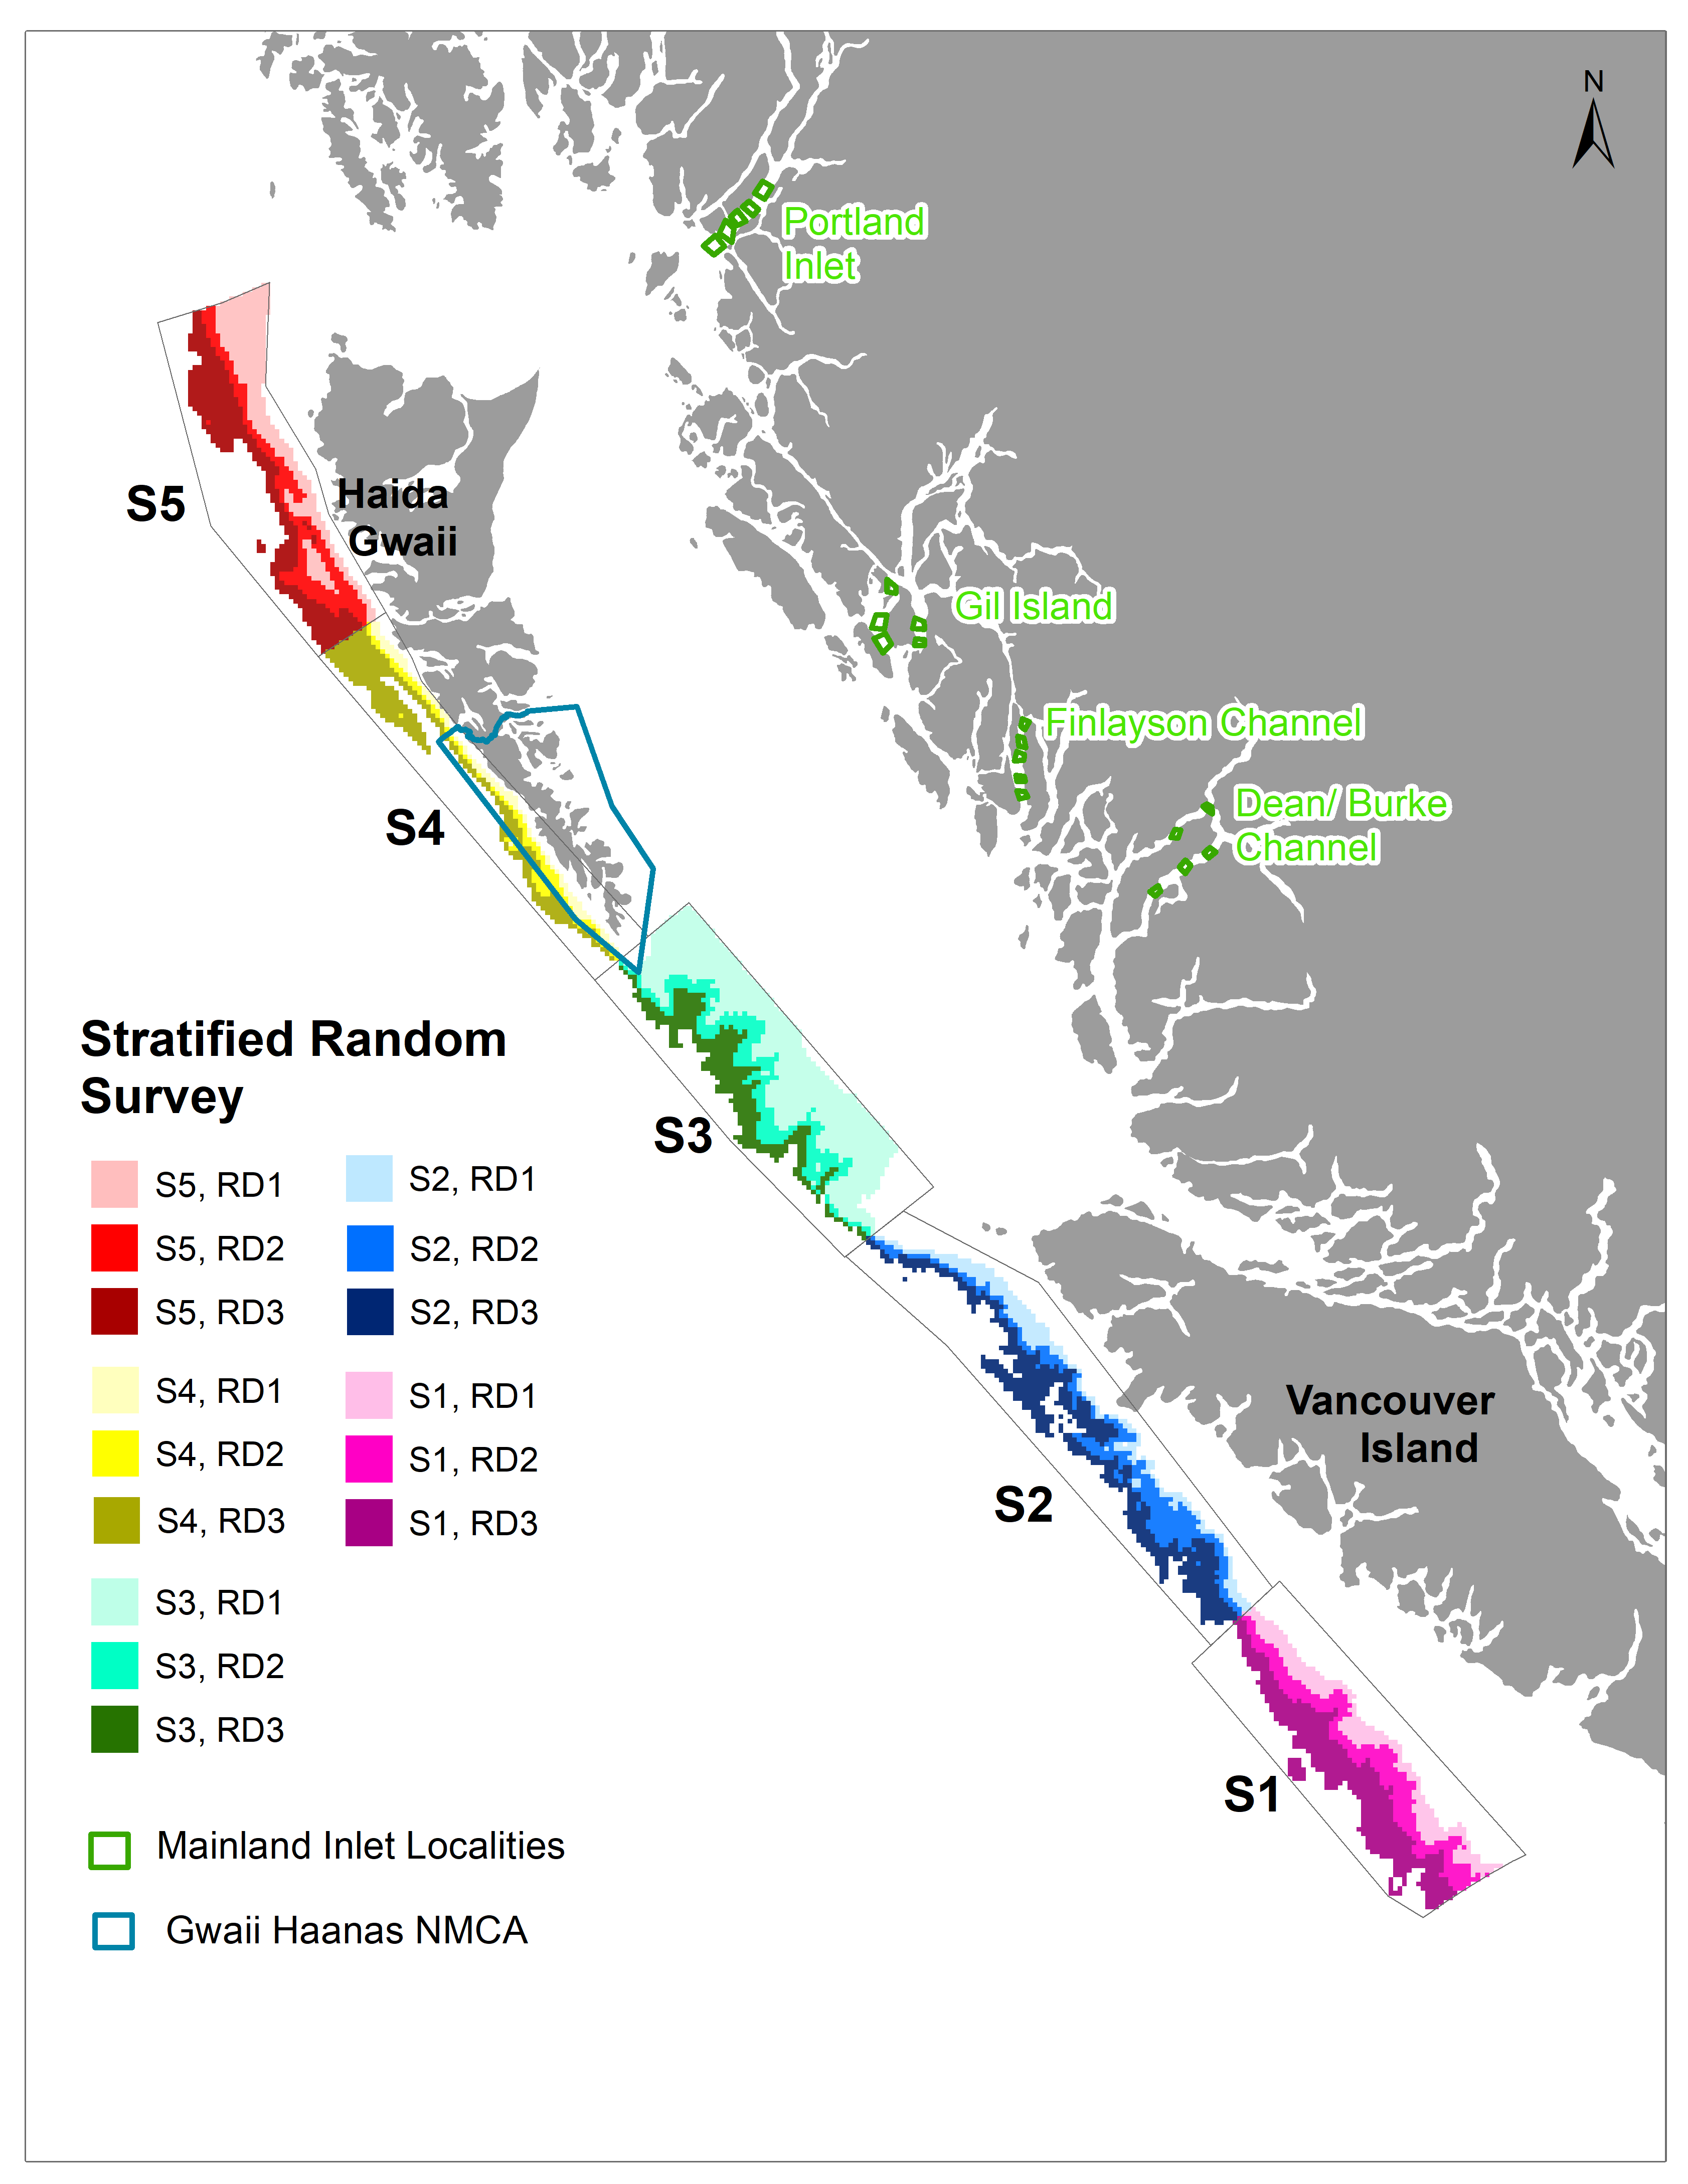
\includegraphics[width=350px]{figures/figure1}}{Figure \ref{fig:figure1}} 

}

\caption{Location of the survey design boundaries of the mainland inlet localities, and the five spatial areas (S\textsubscript{1}-S\textsubscript{5}) of the stratified random survey design. The three depths strata (RD\textsubscript{1}-RD\textsubscript{3}) are colour-coded and nested within each of the five spatial strata.}\label{fig:figure1}
\end{figure}

\begin{figure}[htb]

{\centering \pdftooltip{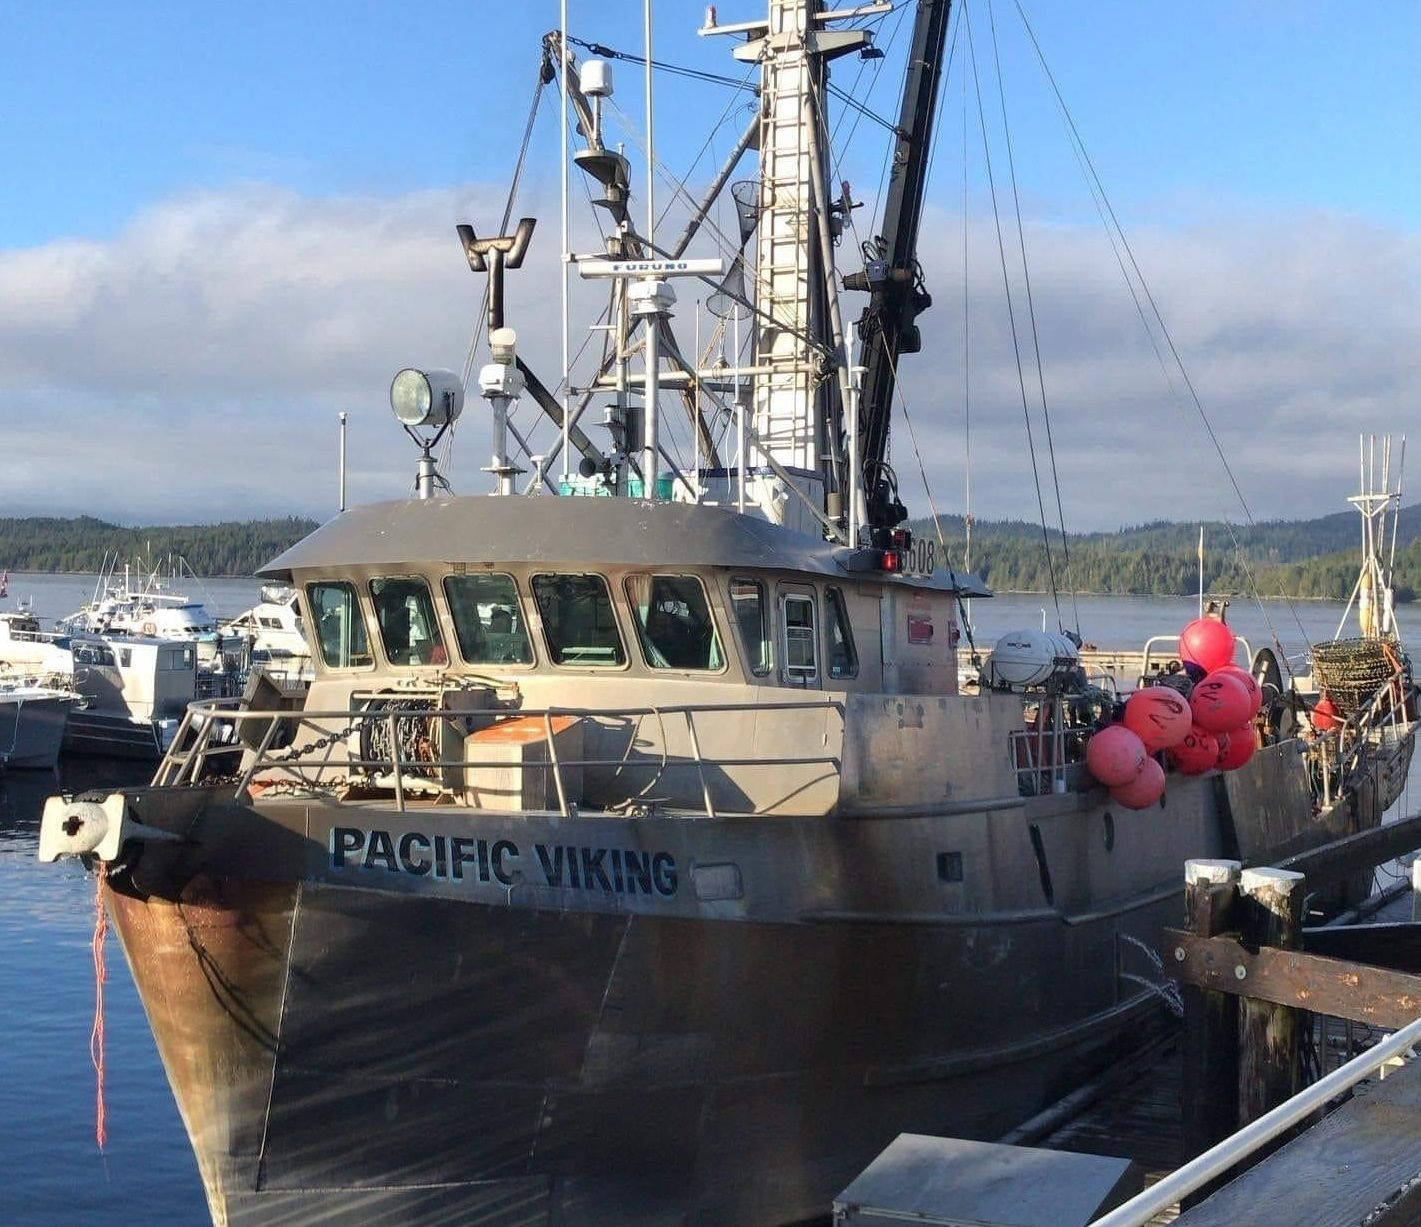
\includegraphics[width=6in,height=200px]{figures/figure2}}{Figure \ref{fig:figure2}} 

}

\caption{Image of the F/V Pacific Viking used for the 2022 Sablefish research and assessment survey. Photo credit: Cody Melnychuk.}\label{fig:figure2}
\end{figure}
\clearpage


\begin{figure}[htb]

{\centering \pdftooltip{\includegraphics[width=450px]{figures/figure3}}{Figure \ref{fig:figure3}} 

}

\caption{Start locations of survey sets (red markers) conducted in 2022 for the stratified random survey areas S\textsubscript{1} through S\textsubscript{5}. Movement/deep-water autonomous camera locations (triangle symbols) are labelled in red font.}\label{fig:figure3}
\end{figure}
\clearpage


\begin{figure}[htb]

{\centering \pdftooltip{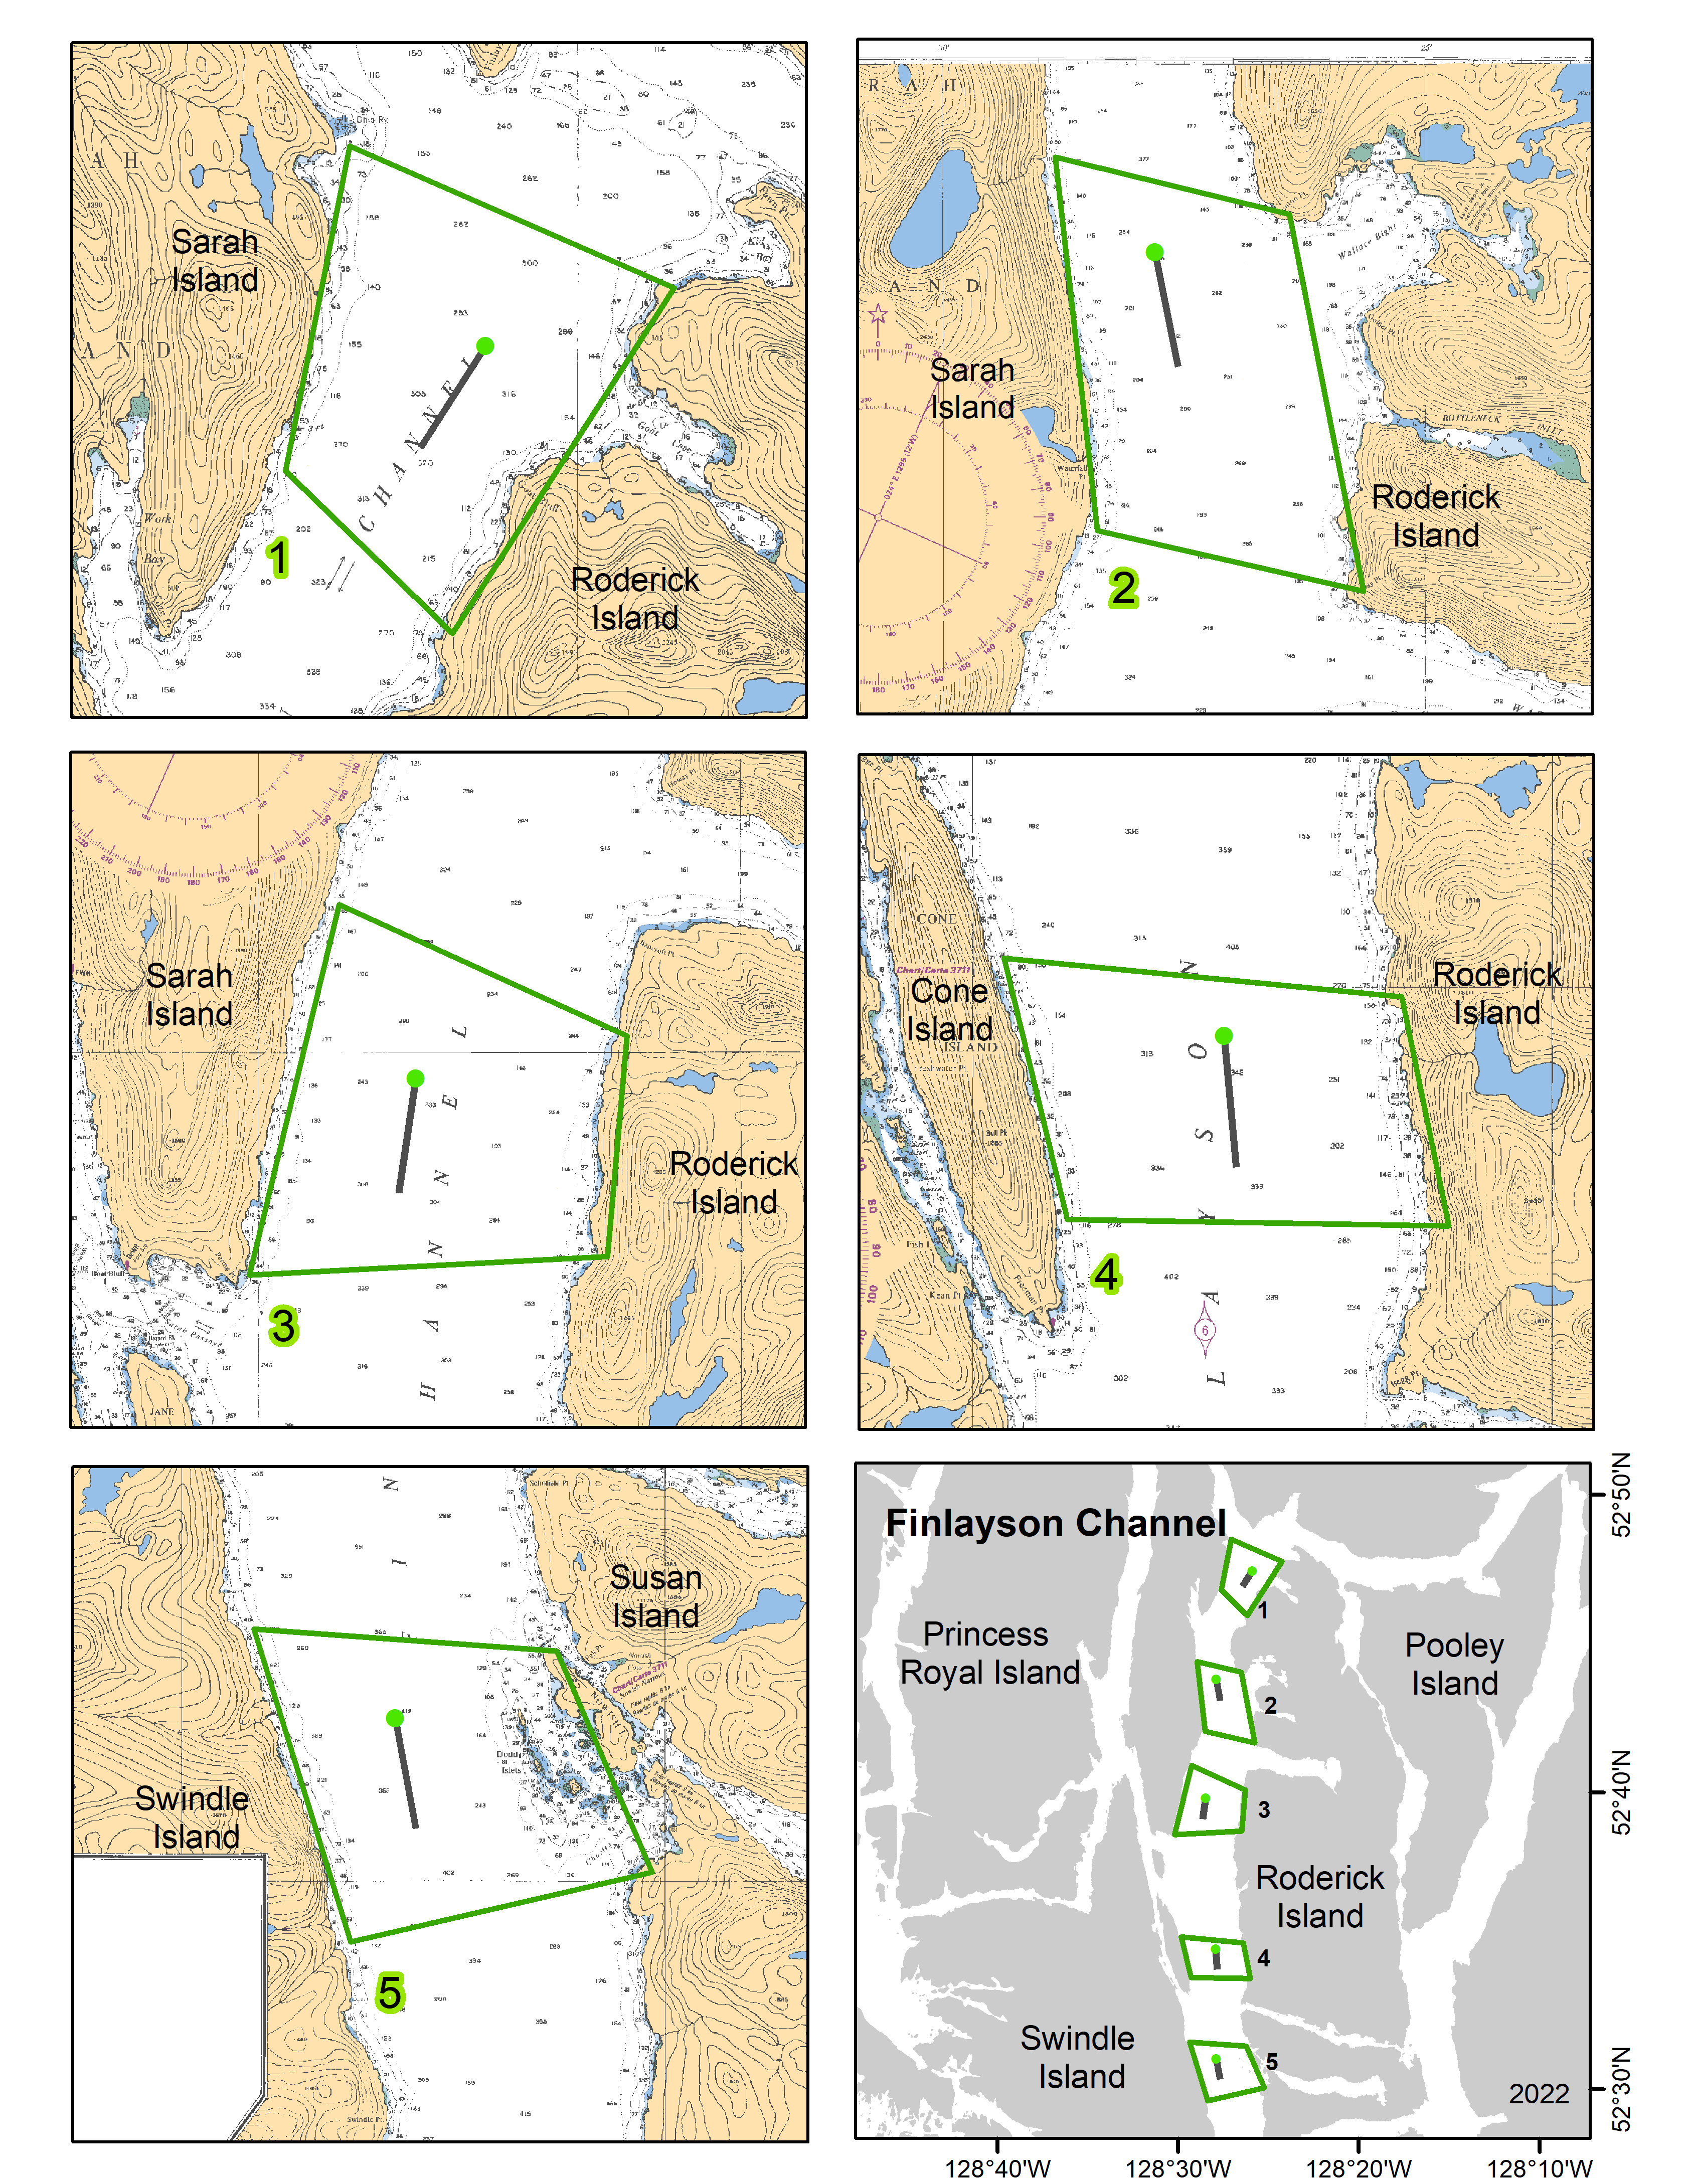
\includegraphics[width=450px]{figures/figure4}}{Figure \ref{fig:figure4}} 

}

\caption{Location of the 2022 standardized sets within the Finlayson Channel mainland inlet locality.}\label{fig:figure4}
\end{figure}
\clearpage


\begin{figure}[htb]

{\centering \pdftooltip{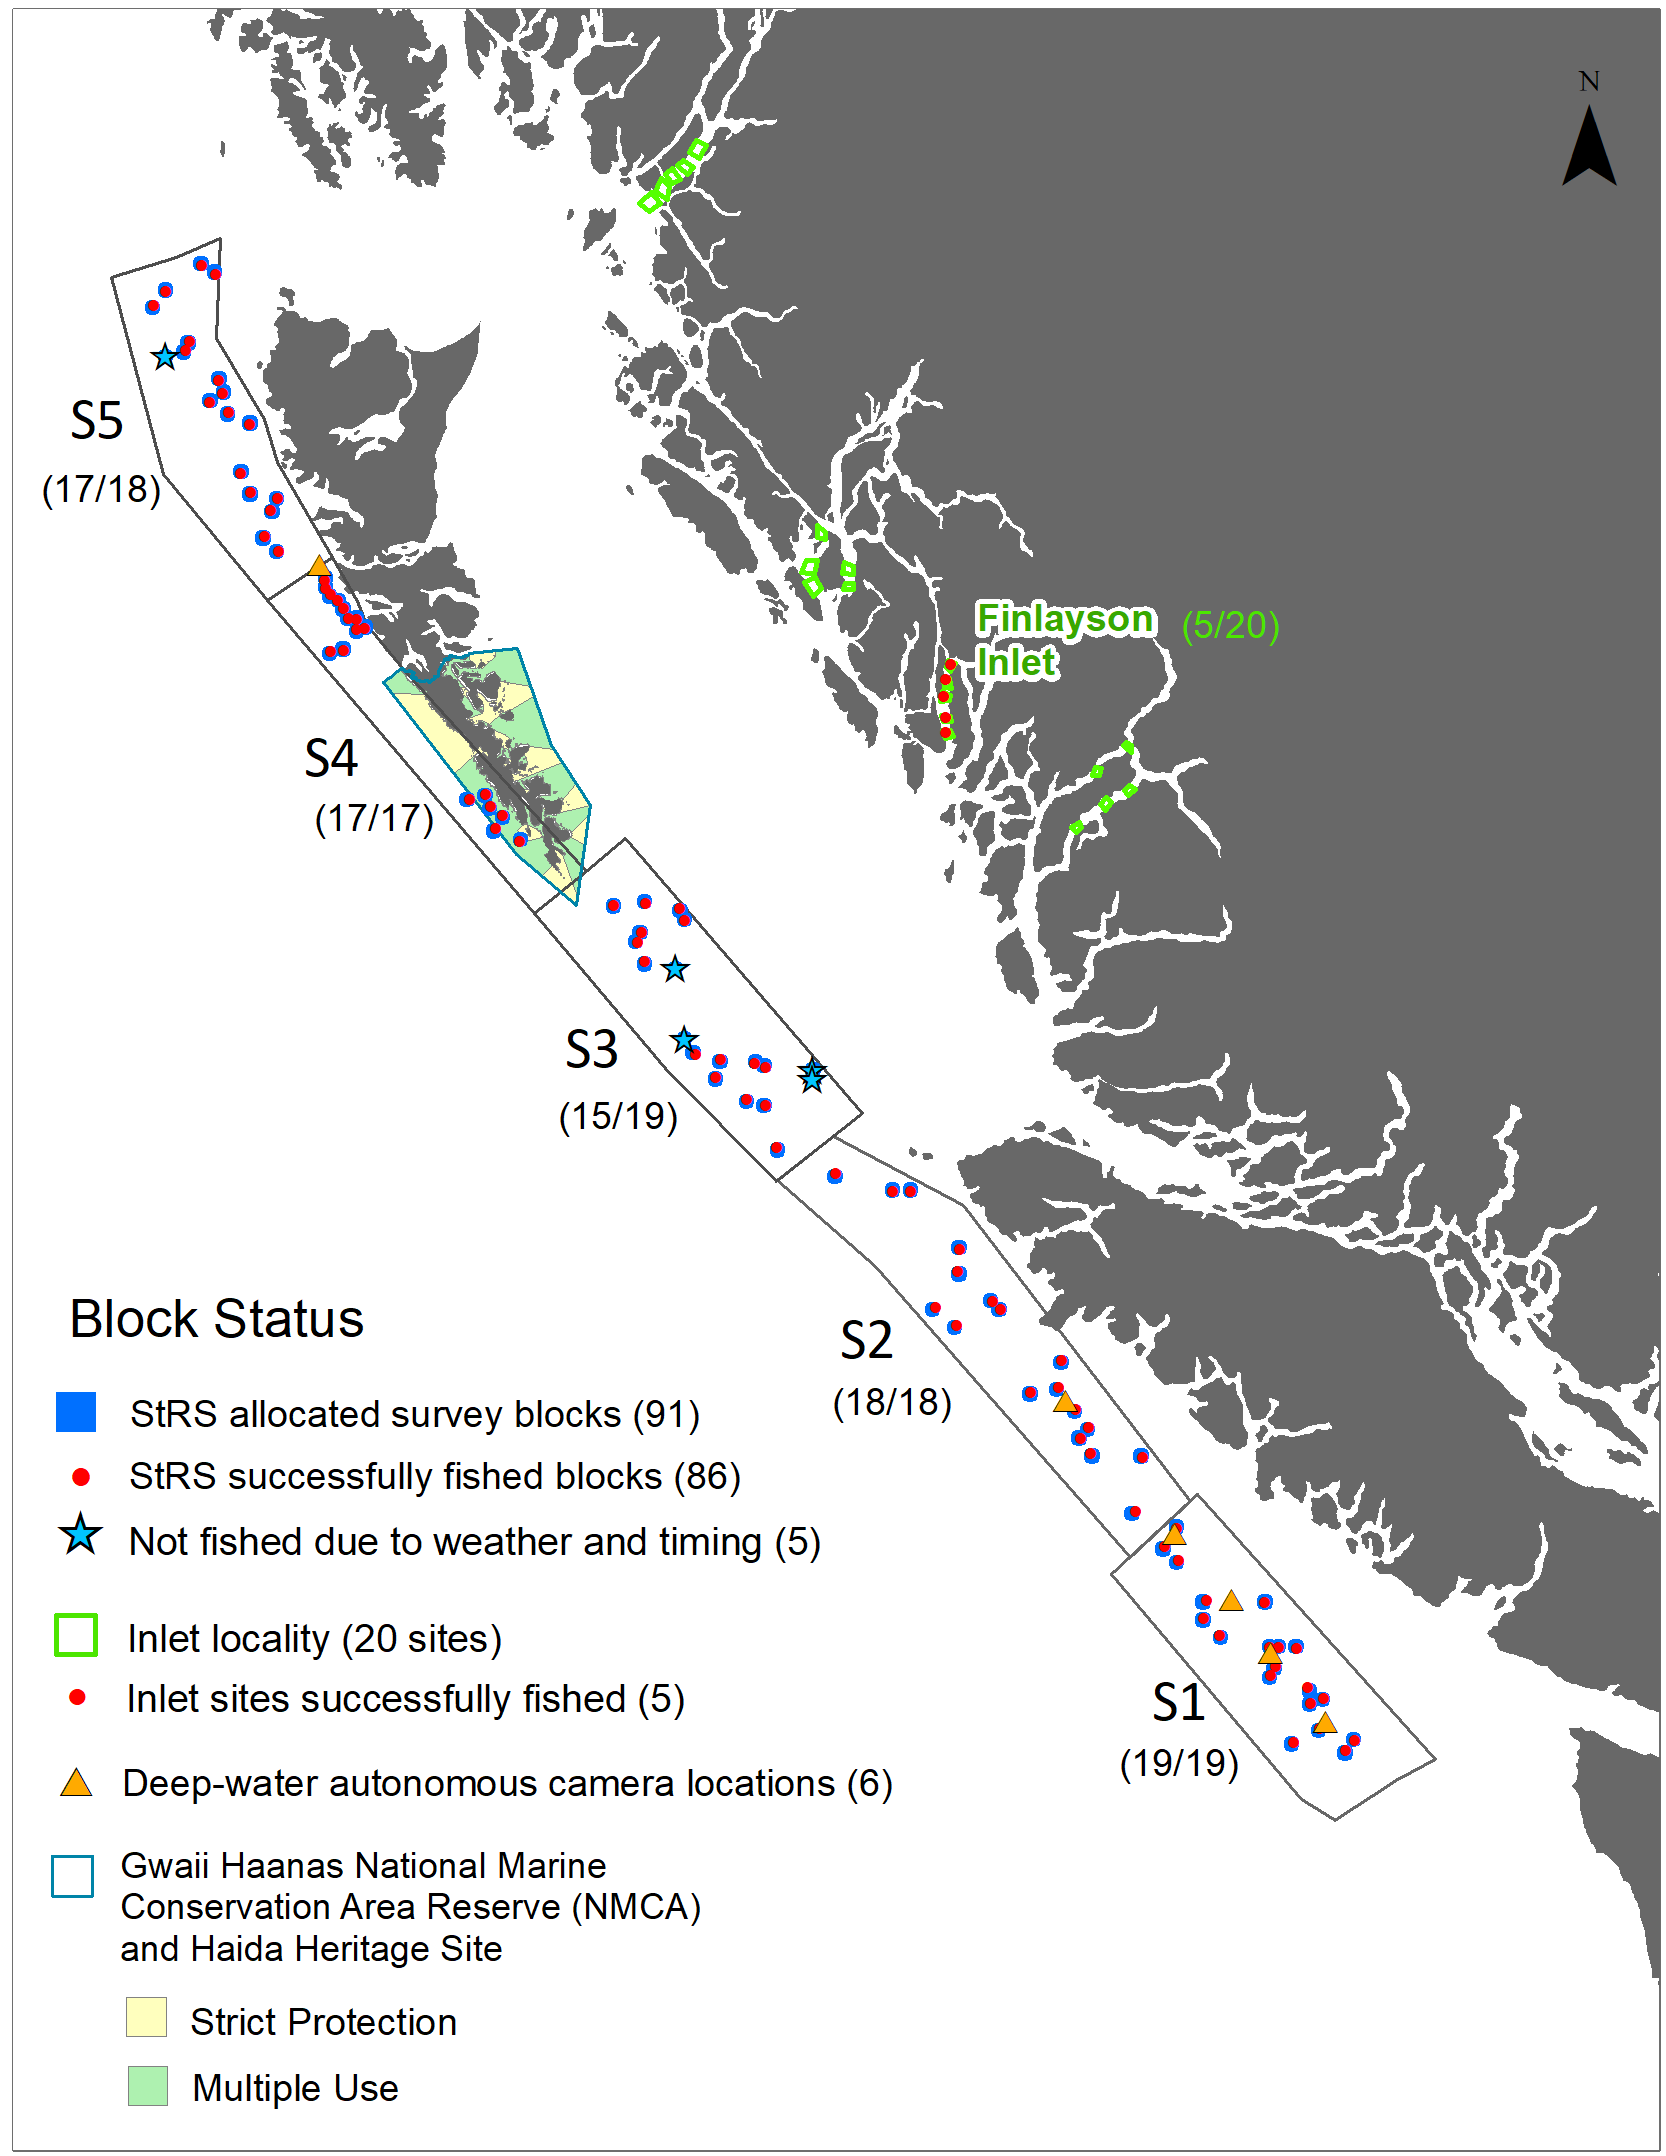
\includegraphics[width=450px]{figures/figure5}}{Figure \ref{fig:figure5}} 

}

\caption{Map of allocated vs completed survey blocks for the 2022 survey sets. Star symbols depict rationale for dropped survey blocks.}\label{fig:figure5}
\end{figure}
\clearpage


\begin{figure}[htb]

{\centering \pdftooltip{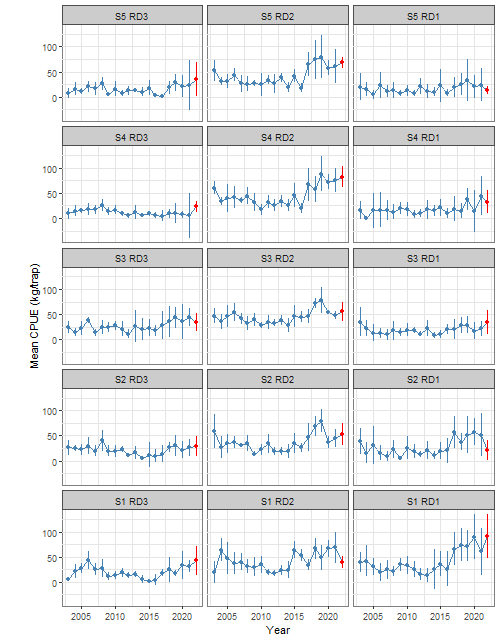
\includegraphics[width=450px]{figures/figure6}}{Figure \ref{fig:figure6}} 

}

\caption{Sablefish maturity.}\label{fig:figure6}
\end{figure}

\begin{figure}[htb]

{\centering \pdftooltip{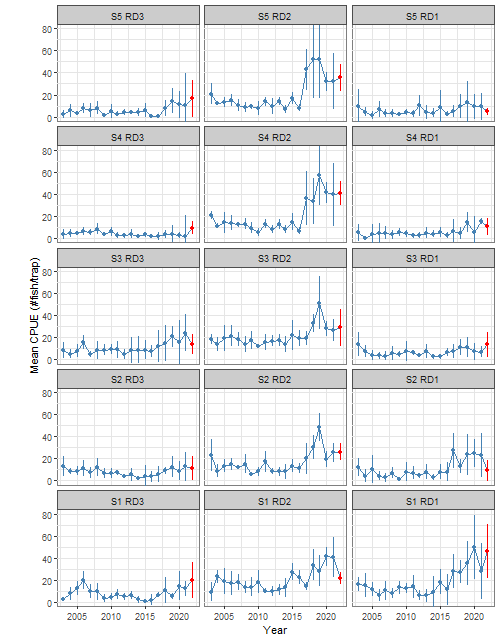
\includegraphics[width=450px]{figures/figure7}}{Figure \ref{fig:figure7}} 

}

\caption{Average Sablefish catch per unit effort (CPUE; mean +/- 95\% CIs) by survey strata since 2003. Panels run deep to shallow (left to right) and north to south (top to bottom).}\label{fig:figure7}
\end{figure}
\clearpage


\begin{figure}[htb]

{\centering \pdftooltip{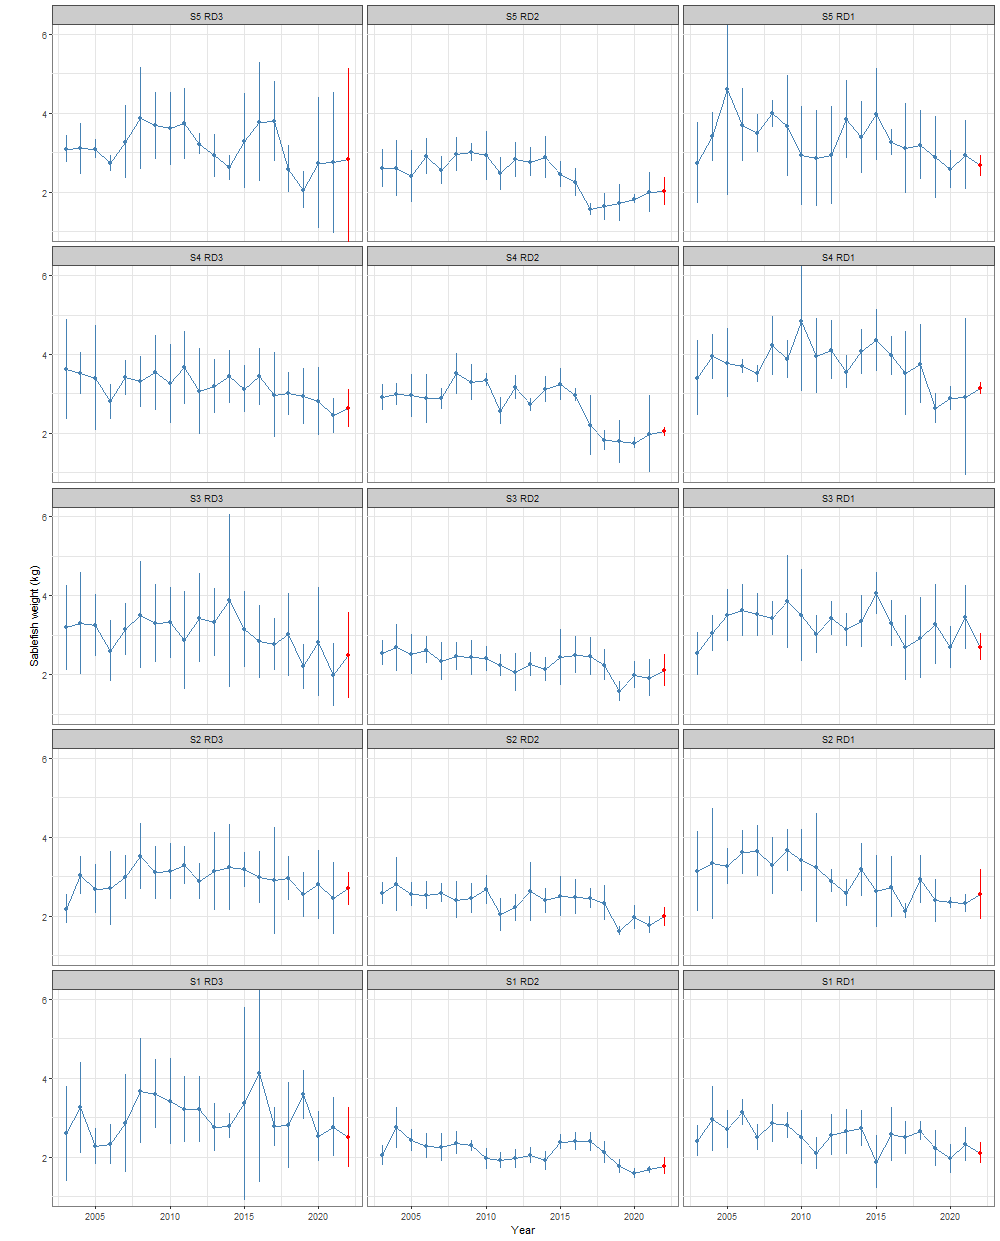
\includegraphics[width=450px,height=576px]{figures/figure8}}{Figure \ref{fig:figure8}} 

}

\caption{Average number of Sablefish per trap (mean +/- 95\% CIs) by StRS survey strata over time. Panels run deep to shallow (left to right) and north to south (top to bottom).}\label{fig:figure8}
\end{figure}
\clearpage


\begin{figure}[htb]

{\centering \pdftooltip{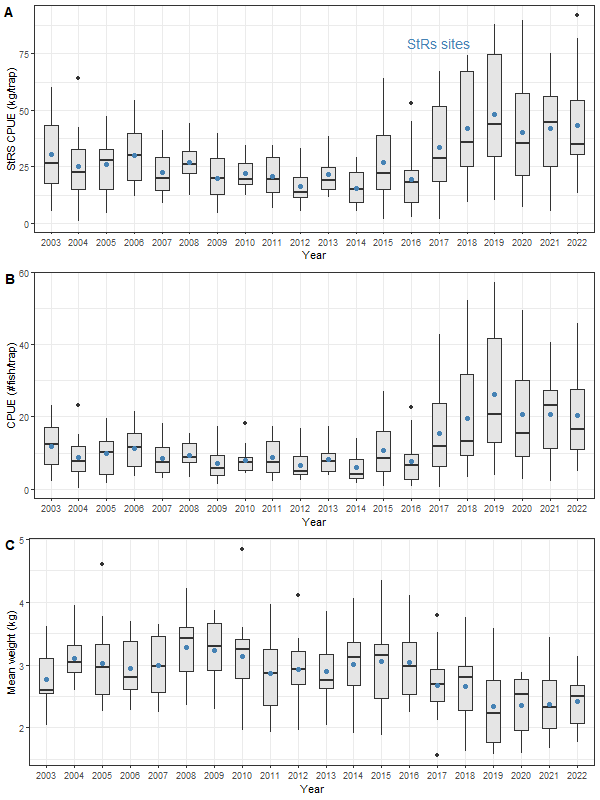
\includegraphics[width=450px,height=576px]{figures/figure9}}{Figure \ref{fig:figure9}} 

}

\caption{Average weight of Sablefish (mean +/- 95\% CIs) by survey strata over time. Panels run deep to shallow (left to right) and north to south (top to bottom).}\label{fig:figure9}
\end{figure}
\clearpage


\begin{figure}[htb]

{\centering \pdftooltip{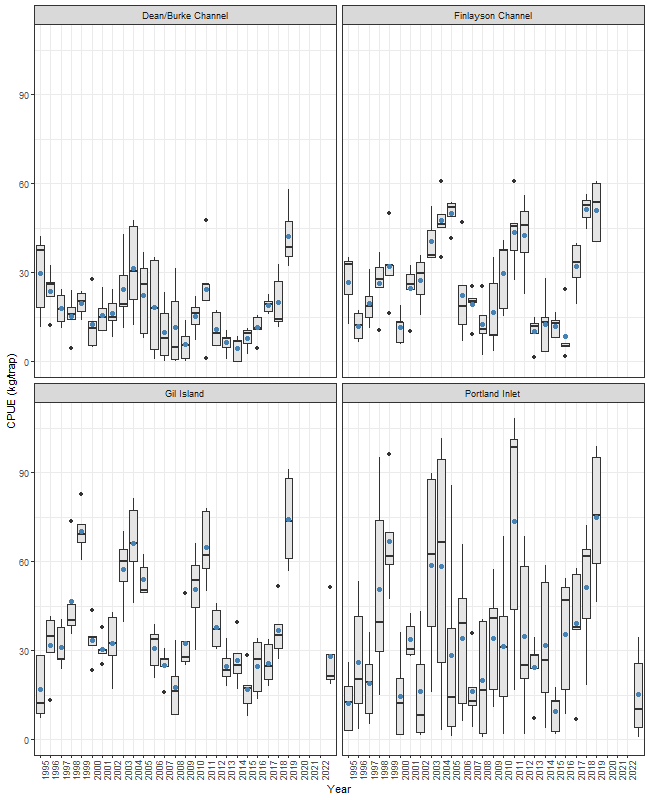
\includegraphics[width=450px,height=576px]{figures/figure10}}{Figure \ref{fig:figure10}} 

}

\caption{(A) Annual mean weight of Sablefish per trap (kg/trap); (B) annual mean number of Sablefish per trap (\#fish/trap); (C) annual mean weight of Sablefish (kg) by StRS survey strata over time. Horizontal line is median and blue dots are arithmetic mean.}\label{fig:figure10}
\end{figure}
\clearpage


\begin{figure}[htb]

{\centering \pdftooltip{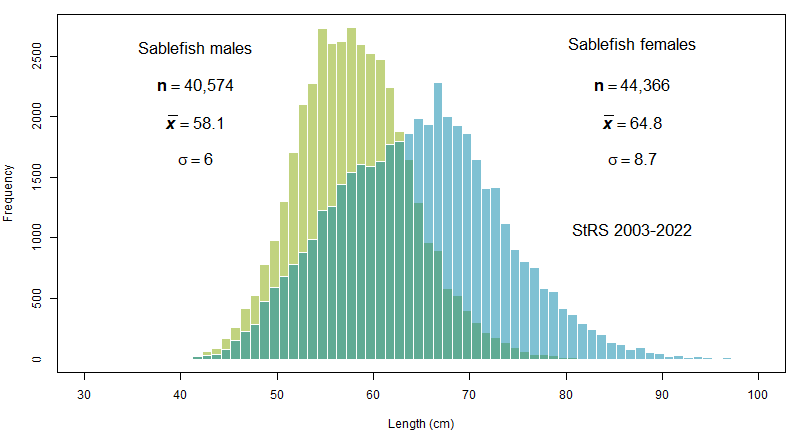
\includegraphics[width=450px,height=560px]{figures/figure11}}{Figure \ref{fig:figure11}} 

}

\caption{Annual distributions of catch statistics over all mainland inlet indexing sets between 1994 and 2019, including: (A) CPUE in units of weight of Sablefish per trap (kg/trap); (B) CPUE in units of Sablefish per trap (\#fish/trap); and (C) mean Sablefish body weight (kg). Horizontal line is median, grey shading shows the 25th and 75\% percentiles, and blue dots show arithmetic means. No inlets were surveyed in 2020. Dean/Burke Channel inlet was the only inlet surveyed in 2021; Finlayson Inlet was the only inlet surveyed in 2022. They are not included in these figures.}\label{fig:figure11}
\end{figure}
\clearpage


\begin{figure}[htb]

{\centering \pdftooltip{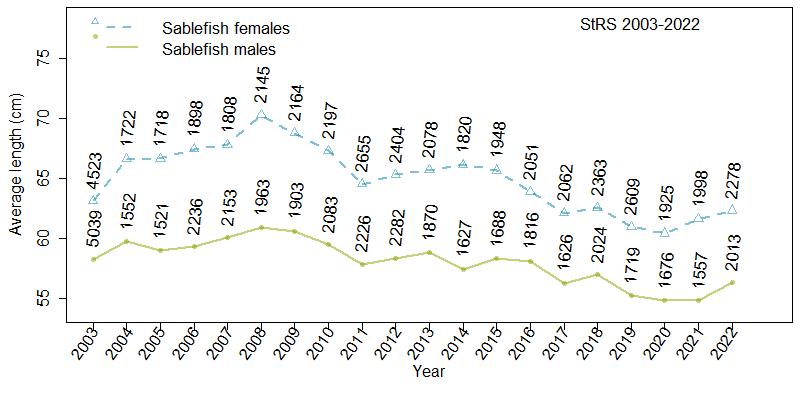
\includegraphics[width=420px,height=245px]{figures/figure12}}{Figure \ref{fig:figure12}} 

}

\caption{Length frequencies for female (grey) and male Sablefish (steel blue) up to 2022 for all StRS sets. Specimen number (n), mean (\(\overline{x}\)) and standard deviation (\(\sigma\)) are displayed.}\label{fig:figure12}
\end{figure}

\begin{figure}[htb]

{\centering \pdftooltip{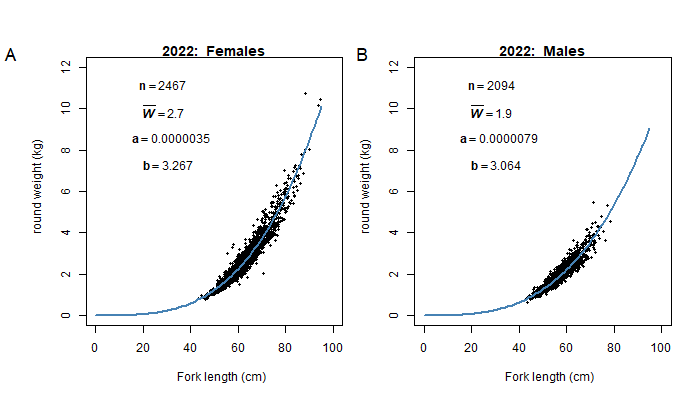
\includegraphics[width=450px,height=250px]{figures/figure13}}{Figure \ref{fig:figure13}} 

}

\caption{Average length of male and female Sablefish by year. Counts by sex are labelled on top of the plotted lines.}\label{fig:figure13}
\end{figure}
\clearpage


\begin{figure}[htb]

{\centering \pdftooltip{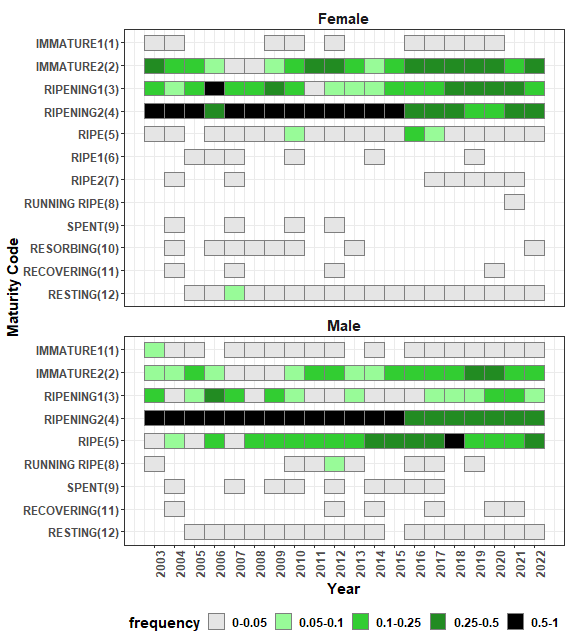
\includegraphics[width=410px,height=235px]{figures/figure14}}{Figure \ref{fig:figure14}} 

}

\caption{Sablefish fork length (L in cm) vs weight (W in kg) for females (A) and males (B) for the 2022 survey.}\label{fig:figure14}
\end{figure}

\begin{figure}[htb]

{\centering \pdftooltip{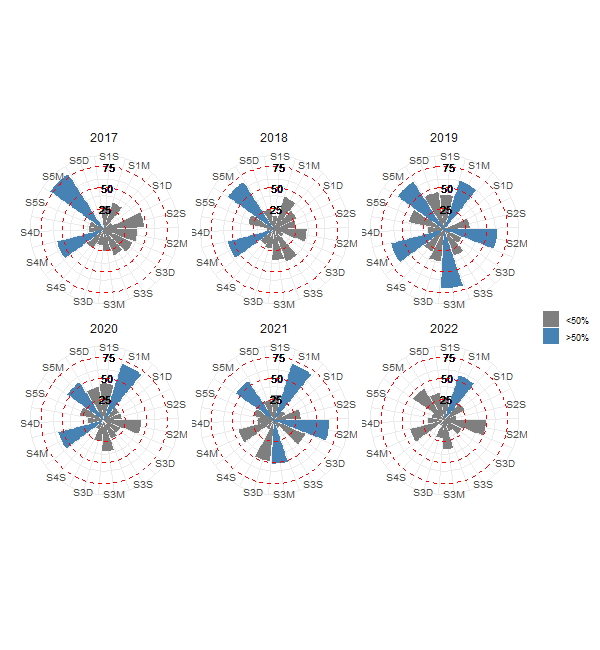
\includegraphics[width=350px,height=235px]{figures/figure15}}{Figure \ref{fig:figure15}} 

}

\caption{The percentage of sub-legal Sablefish (\textless55 cm fork length) sampled by spatial (S\textsubscript{1}-S\textsubscript{5}) and depth strata (S=shallow, RD\textsubscript{1}; M=mid, RD\textsubscript{2}; D=deep, RD\textsubscript{3}) over time. Sub-legal specimen count above 50\% sampled shown in blue.}\label{fig:figure15}
\end{figure}
\clearpage


\begin{figure}[htb]

{\centering \pdftooltip{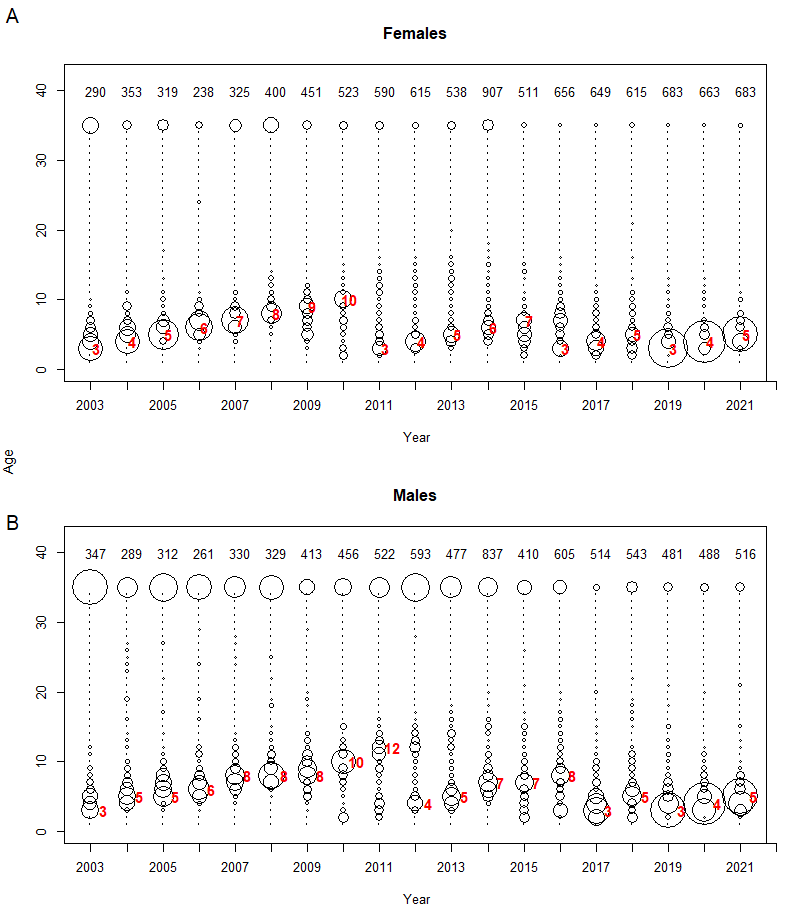
\includegraphics[width=500px,height=577px]{figures/figure16}}{Figure \ref{fig:figure16}} 

}

\caption{Bubble plot for female (A) and male (B) Sablefish ages by survey year from StRS sets that have been aged. The sizes of the circles are proportional to the number of fish with given ages. Fish age 35 and older are included in one bubble. The total number of fish aged are listed across the top of each panel. The ages with the highest ratios are posted to the right of each bubble.}\label{fig:figure16}
\end{figure}
\clearpage


\begin{figure}[htb]

{\centering \pdftooltip{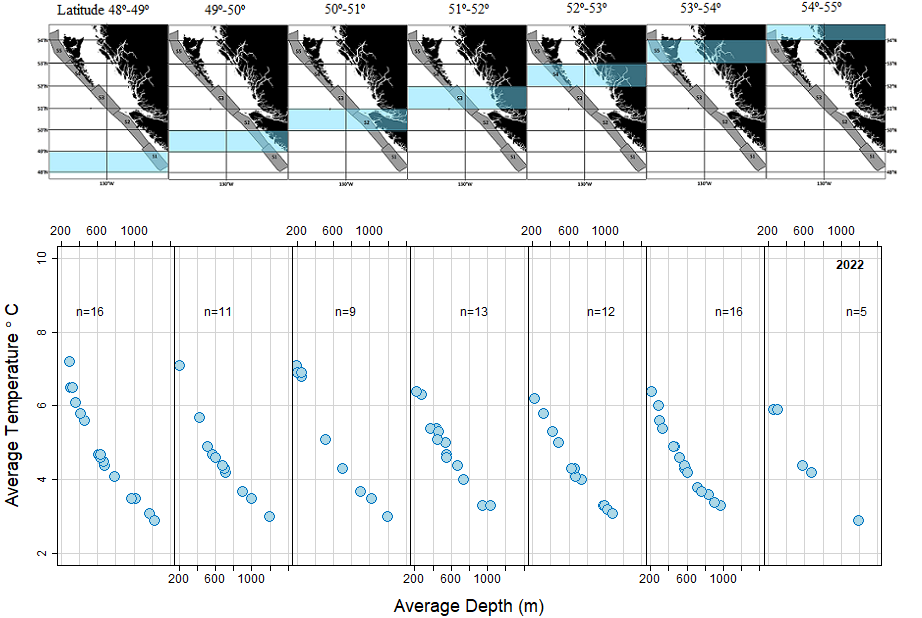
\includegraphics[width=500px,height=335px]{figures/figure17}}{Figure \ref{fig:figure17}} 

}

\caption{Coplot of average depth (m) vs average temperature (\(^\circ\)C) for a given 1-degree latitude range (blue bands) for 2022. The number of fishing sets deployed with a SBE 39 recorder are represented by n.}\label{fig:figure17}
\end{figure}
\clearpage


\begin{figure}[htb]

{\centering \pdftooltip{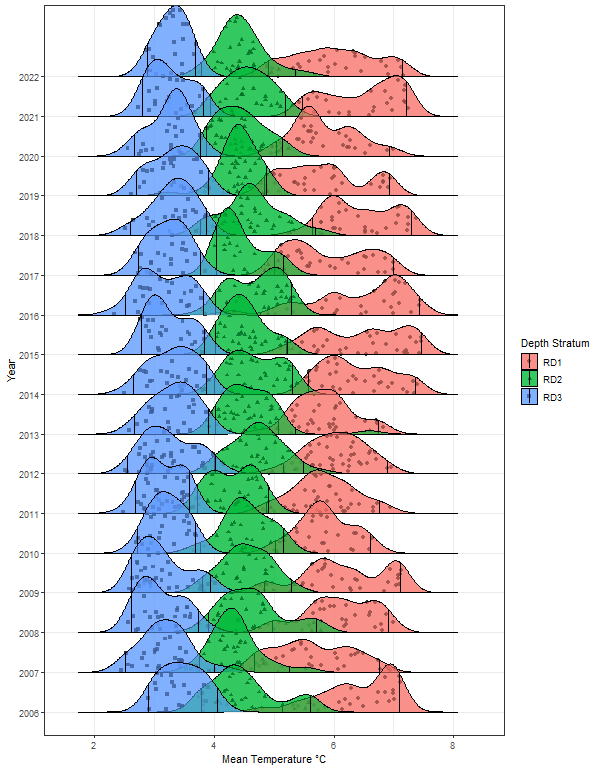
\includegraphics[width=480px,height=616px]{figures/figure18}}{Figure \ref{fig:figure18}} 

}

\caption{Vertical density ridgeplots of mean temperatures per year as reported by set from the Sea-bird SBE 39 loggers on traps at three depth intervals, RD\textsubscript{1} = shallow (100-450 m), RD\textsubscript{2} = mid (450-850 m), RD\textsubscript{3} = deep (850-1400 m). Lines indicate the 2.5\% and 97.5\% tails.}\label{fig:figure18}
\end{figure}
\clearpage

\begin{appendices}
\counterwithin{figure}{section}
\counterwithin{table}{section}
\counterwithin{equation}{section}

\clearpage

\section{LIST OF SABLEFISH RESEARCH AND ASSESSMENT SURVEYS.}
\label{app:first-appendix}

\begingroup\fontsize{8}{10}\selectfont
\begin{longtable}{rlllrr}
\toprule
\textbf{Year} & \textbf{Dates} & \textbf{Vessel} & \textbf{Captain} & \textbf{Set Count} & \textbf{GFBIO Trip id}\\
\midrule
1988 & Oct 28  - Nov 24 & VICIOUS FISHER & VANCE FLETCHER & 16 & 43990\\
1989 & Oct 19  - Nov 18 & LA PORSCHE & SIGURD BRYNJOLFSON & 29 & 43910\\
1990 & Nov  8  - Nov 18 & VIKING STAR & DOUG FARRINGTON & 24 & 43750\\
1991 & Oct  9  - Oct 29 & W. E. RICKER & ALAN FARRINGTON & 32 & 43673\\
1992 & Oct 13  - Nov  4 & W. E. RICKER & RON ROBERTS & 38 & 43670\\
1993 & Oct 19  - Nov 11 & W. E. RICKER & ALAN FARRINGTON & 42 & 43650\\
1994 & Oct 13  - Oct 31 & LA PORSCHE & RICHARD BEAUVAIS & 39 & 43630\\
1994 & Oct 18  - Nov 13 & WESTERN VIKING & RICK JONES & 27 & 43390\\
1995 & Oct  8  - Oct 20 & OCEAN PEARL & ROBERT FRAUMENI & 29 & 43270\\
1995 & Oct 11  - Oct 28 & VICTOR F & MICHAEL DERRY & 34 & 43330\\
1995 & Oct  1  - Oct 31 & VIKING SUNRISE & JASON OLSEN & 40 & 43350\\
1996 & Sep 26  - Oct 10 & OCEAN PEARL & MICHAEL DERRY & 32 & 43039\\
1996 & Sep 30  - Oct 22 & VIKING STAR & OTTO ELVAN & 49 & 43210\\
1996 & May 10  - May 30 & VIKING SUNRISE & ALBERT (DEACON) MELNYCHUK & 42 & 43024\\
1997 & Sep 26  - Oct 21 & OCEAN PEARL & MICHAEL DERRY & 74 & 42699\\
1997 & May 20  - Jun 10 & VIKING SUNRISE & ALBERT (DEACON) MELNYCHUK & 42 & 42760\\
1998 & Sep 22  - Oct 17 & OCEAN PEARL & MICHAEL DERRY & 89 & 41122\\
1999 & Sep 29  - Oct 30 & OCEAN PEARL & MICHAEL DERRY & 109 & 40589\\
2000 & Oct  8  - Nov 14 & PACIFIC VIKING & ALBERT (DEACON) MELNYCHUK & 131 & 40517\\
2001 & Oct  6  - Nov  6 & OCEAN PEARL & MICHAEL DERRY & 134 & 43233\\
2002 & Oct  4  - Nov  7 & PACIFIC VIKING & ALBERT (DEACON) MELNYCHUK & 125 & 48120\\
2002 & Oct  5  - Nov 13 & VIKING SUNRISE & JASON OLSEN & 90 & 48110\\
2003 & Oct 15  - Nov 13 & OCEAN PEARL & MICHAEL DERRY & 94 & 52100\\
2003 & Oct  7  - Nov 10 & VIKING STAR & JIM FARRINGTON & 84 & 52120\\
2004 & Oct  5  - Nov 15 & MILBANKE SOUND & DON QUAST & 95 & 58145\\
2004 & Oct  5  - Nov  3 & OCEAN MARAUDER & ALBERT (DEACON) MELNYCHUK & 84 & 57360\\
2005 & Oct  4  - Nov  2 & PACIFIC VIKING & ALBERT (DEACON) MELNYCHUK & 84 & 60529\\
2005 & Oct  7  - Nov 17 & VIKING SUNRISE & RORY JOHNSON & 88 & 60503\\
2006 & Oct  1  - Nov  1 & PACIFIC VIKING & ALBERT (DEACON) MELNYCHUK & 98 & 62966\\
2006 & Oct  2  - Nov 15 & SENA II & TIM JOYS & 98 & 62666\\
2007 & Oct  7  - Nov 12 & PACIFIC VIKING & ALBERT (DEACON) MELNYCHUK & 99 & 65106\\
2007 & Oct  8  - Nov 12 & VIKING TIDE & JASON OLSEN & 91 & 65107\\
2008 & Sep 29  - Nov 16 & OCEAN PEARL & ROBERT FRAUMENI & 157 & 67007\\
2009 & Oct  8  - Nov 25 & OCEAN PEARL & ROBERT FRAUMENI & 155 & 69067\\
2010 & Oct  9  - Nov 30 & OCEAN PEARL & ROBERT FRAUMENI & 153 & 70787\\
2011 & Oct  9  - Nov 21 & OCEAN PEARL & DARCY NICHOLS & 132 & 72067\\
2012 & Oct  9  - Nov 17 & OCEAN PEARL & DARCY NICHOLS & 135 & 73190\\
2013 & Oct 11  - Nov 17 & PACIFIC VIKING & ALBERT (DEACON) MELNYCHUK & 111 & 74872\\
2014 & Oct  9  - Nov 17 & OCEAN PEARL & DARCY NICHOLS & 111 & 76150\\
2015 & Oct  9  - Nov 20 & PACIFIC VIKING & ALBERT (DEACON) MELNYCHUK & 111 & 77830\\
2016 & Oct  7  - Nov 22 & OCEAN PEARL & DARCY NICHOLS & 111 & 80471\\
2017 & Oct  6  - Nov 21 & PACIFIC VIKING & ALBERT (DEACON) MELNYCHUK & 109 & 82790\\
2018 & Oct  9  - Nov 19 & OCEAN PEARL & DARCY NICHOLS & 111 & 84250\\
2019 & Oct  8  - Nov 25 & PACIFIC VIKING & ALBERT (DEACON) MELNYCHUK & 109 & 85230\\
2020 & Oct  7  - Nov 21 & PACIFIC VIKING & ALBERT (DEACON) MELNYCHUK & 87 & 85690\\
2021 & Oct  6  - Nov 21 & PACIFIC VIKING & ALBERT (DEACON) MELNYCHUK & 81 & 86130\\
2022 & Oct  3  - Nov 19 & PACIFIC VIKING & ALBERT (DEACON) MELNYCHUK & 97 & 86530\\
\bottomrule
\end{longtable}
\endgroup{}
\clearpage

\section{SURVEY SET DETAILS 2022.}
\label{app:second-appendix}

Details of sets completed during the 2022 survey program (F/V Pacific Viking). Sets are listed by stratum/inlet name, set type, depth stratum, start date, end of gear deployment time and duration in minutes. The depth strata for type 3 tagging sets include RD\textsubscript{1} (100-250 fathoms), RD\textsubscript{2} (250-450 fathoms) and RD\textsubscript{3} (450-750 fathoms). The position data includes the major area and start and end latitude and longitude in degrees decimal minutes. The bottom depths (in meters) of the fishing set are shown with the mean bottom depth calculated from recordings at one minute intervals between the start and end of the set. The number of traps fished for each set excludes open traps, while holed or fouled traps have been included. Sets that successfully deployed a Seabird SBE temperature and pressure recorder (SBE 39), an accelerometer (AXL) or a camera (CAM) are indicated with an `x'.
\begin{landscape}\begingroup\fontsize{8}{10}\selectfont
\begin{longtable}{>{\raggedright\arraybackslash}p{0.5cm}>{\raggedright\arraybackslash}p{1.3cm}>{\raggedright\arraybackslash}p{0.9cm}>{\raggedright\arraybackslash}p{0.7cm}>{\raggedright\arraybackslash}p{0.9cm}>{\raggedright\arraybackslash}p{0.6cm}>{\raggedright\arraybackslash}p{0.9cm}>{\raggedright\arraybackslash}p{0.5cm}>{\raggedright\arraybackslash}p{1.2cm}>{\raggedright\arraybackslash}p{1.6cm}>{\raggedright\arraybackslash}p{1.2cm}>{\raggedright\arraybackslash}p{1.6cm}>{\raggedright\arraybackslash}p{0.6cm}>{\raggedright\arraybackslash}p{0.6cm}>{\raggedright\arraybackslash}p{0.5cm}>{\raggedright\arraybackslash}p{0.6cm}>{\raggedright\arraybackslash}p{0.4cm}>{\raggedright\arraybackslash}p{0.4cm}>{\raggedright\arraybackslash}p{0.4cm}}
\toprule
\textbf{Set} & \textbf{Spatial Stratum} & \textbf{Type} & \textbf{Depth Stratum} & \textbf{Date} & \textbf{Time} & \textbf{Duration (minutes)} & \textbf{Area} & \textbf{Start Latitude} & \textbf{Start Longitude} & \textbf{End Latitude} & \textbf{End Longitude} & \textbf{Start Depth (m)} & \textbf{End Depth (m)} & \textbf{Mean Depth (m)} & \textbf{Traps Fished} & \textbf{SBE 39} & \textbf{AXL} & \textbf{CAM}\\
\midrule
\endfirsthead
\multicolumn{19}{@{}l}{continued.}\\
\toprule
\textbf{Set} & \textbf{Spatial Stratum} & \textbf{Type} & \textbf{Depth Stratum} & \textbf{Date} & \textbf{Time} & \textbf{Duration (minutes)} & \textbf{Area} & \textbf{Start Latitude} & \textbf{Start Longitude} & \textbf{End Latitude} & \textbf{End Longitude} & \textbf{Start Depth (m)} & \textbf{End Depth (m)} & \textbf{Mean Depth (m)} & \textbf{Traps Fished} & \textbf{SBE 39} & \textbf{AXL} & \textbf{CAM}\\
\midrule
\endhead

\endfoot
\bottomrule
\endlastfoot
1 & S1 & StRS & RD1 & Oct  5 & 08:06 & 1326 & 3C & 48° 3.4'N & 126° 0.9'W & 48° 3.3'N & 126° 1.8'W & 302 & 281 & 300 & 25 & x &  & \\
2 & S1 & StRS & RD2 & Oct  5 & 09:26 & 1366 & 3C & 48° 1'N & 126° 4.4'W & 48° 0.8'N & 126° 5.3'W & 496 & 471 & 472 & 25 & x &  & \\
3 & S1 & StRS & RD3 & Oct  5 & 11:54 & 1393 & 3C & 48° 3.4'N & 126° 23.3'W & 48° 3.4'N & 126° 24.3'W & 1230 & 1277 & 1254 & 25 & x &  & \\
4 & S1 & StRS & RD2 & Oct  5 & 13:54 & 1535 & 3C & 48° 6.6'N & 126° 13.7'W & 48° 6.5'N & 126° 14.6'W & 656 & 695 & 676 & 25 & x &  & \\
5 &  & Movement &  & Oct  5 & 15:08 & 1327 & 3C & 48° 8'N & 126° 11.6'W & 48° 8.1'N & 126° 13.9'W & 466 & 603 & 529 & 58 & x & x & x\\
6 & S1 & StRS & RD2 & Oct  5 & 16:36 & 1485 & 3C & 48° 2.7'N & 126° 16.7'W & 48° 2.6'N & 126° 17.7'W & 665 & 687 & 676 & 25 & x & x & x\\
7 & S1 & StRS & RD2 & Oct  5 & 18:00 & 1487 & 3C & 48° 3.8'N & 126° 11.7'W & 48° 3.5'N & 126° 12.7'W & 479 & 639 & 567 & 25 & x &  & \\
8 & S1 & StRS & RD2 & Oct  7 & 08:07 & 1323 & 3C & 48° 6.8'N & 126° 17.4'W & 48° 6.2'N & 126° 17.9'W & 565 & 700 & 617 & 25 & x &  & \\
9 & S1 & StRS & RD3 & Oct  7 & 10:23 & 1345 & 3C & 48° 9.8'N & 126° 30.9'W & 48° 9.7'N & 126° 31.8'W & 1012 & 1035 & 1025 & 25 & x &  & \\
10 & S1 & StRS & RD2 & Oct  7 & 11:50 & 1349 & 3C & 48° 2'N & 126° 29.2'W & 48° 1.7'N & 126° 30.1'W & 661 & 669 & 648 & 25 & x &  & \\
11 &  & Movement &  & Oct  7 & 13:39 & 1343 & 3C & 48° 5.4'N & 126° 31'W & 48° 4.7'N & 126° 32.9'W & 415 & 562 & 479 & 58 & x & x & x\\
12 & S1 & StRS & RD1 & Oct  7 & 15:04 & 1464 & 3C & 48° 6.6'N & 126° 31.1'W & 48° 6.5'N & 126° 32'W & 336 & 378 & 355 & 25 & x & x & x\\
13 & S1 & StRS & RD1 & Oct  7 & 16:22 & 1556 & 3C & 48° 6.7'N & 126° 27.8'W & 48° 6.4'N & 126° 28.7'W & 294 & 315 & 305 & 25 & x &  & \\
14 & S1 & StRS & RD1 & Oct  7 & 17:53 & 1578 & 3C & 48° 6.3'N & 126° 21'W & 48° 6.2'N & 126° 22.1'W & 306 & 333 & 325 & 25 & x &  & \\
15 & S1 & StRS & RD1 & Oct  9 & 08:04 & 1328 & 3C & 48° 7.9'N & 126° 32.4'W & 48° 7.4'N & 126° 33.2'W & 272 & 414 & 366 & 25 & x &  & \\
16 & S1 & StRS & RD3 & Oct  9 & 10:35 & 1381 & 3C & 48° 0'N & 126° 49.2'W & 48° 0'N & 126° 50.3'W & 1209 & 1214 & 1198 & 25 & x &  & \\
17 & S1 & StRS & RD3 & Oct  9 & 13:06 & 1355 & 3C & 48° 4.4'N & 126° 54.9'W & 48° 4.3'N & 126° 55.9'W & 965 & 1011 & 990 & 25 & x &  & \\
18 &  & Movement &  & Oct  9 & 14:55 & 1379 & 3C & 48° 8.4'N & 126° 45'W & 48° 8.3'N & 126° 47.4'W & 409 & 530 & 461 & 58 & x & x & x\\
19 & S1 & StRS & RD2 & Oct  9 & 16:01 & 1518 & 3C & 48° 8.7'N & 126° 53.9'W & 48° 8.6'N & 126° 55.1'W & 775 & 821 & 798 & 25 & x & x & x\\
20 & S1 & StRS & RD2 & Oct 11 & 08:02 & 1329 & 3D & 49° 0.6'N & 127° 3.6'W & 49° 0.5'N & 127° 4.6'W & 677 & 747 & 708 & 25 & x &  & \\
21 &  & Movement &  & Oct 11 & 09:31 & 1620 & 3D & 49° 5'N & 127° 5.3'W & 49° 5'N & 127° 7.6'W & 380 & 538 & 464 & 58 & x & x & x\\
22 & S1 & StRS & RD3 & Oct 11 & 10:47 & 1289 & 3D & 49° 2'N & 127° 8.8'W & 49° 1.9'N & 127° 9.8'W & 967 & 1081 & 1025 & 25 & x &  & \\
23 & S1 & StRS & RD1 & Oct 11 & 12:08 & 1318 & 3D & 49° 6.3'N & 127° 4.3'W & 49° 6.3'N & 127° 5.4'W & 197 & 213 & 205 & 25 & x & x & x\\
24 & S2 & StRS & RD3 & Oct 11 & 14:16 & 1567 & 3D & 49° 0.7'N & 127° 19.3'W & 49° 0.7'N & 127° 20.3'W & 1074 & 1199 & 1191 & 25 & x &  & \\
25 & S2 & StRS & RD1 & Oct 11 & 16:51 & 1572 & 3D & 49° 3.8'N & 127° 16.3'W & 49° 4'N & 127° 17.4'W & 313 & 461 & 401 & 25 & x &  & \\
26 & S2 & StRS & RD2 & Oct 11 & 19:15 & 1595 & 3D & 49° 5'N & 127° 35.7'W & 49° 4.2'N & 127° 36'W & 539 & 762 & 670 & 25 & x &  & \\
27 & S2 & StRS & RD2 & Oct 13 & 08:01 & 1331 & 3D & 49° 8.8'N & 127° 39.3'W & 49° 8.7'N & 127° 40.4'W & 524 & 580 & 529 & 25 & x &  & \\
28 & S2 & StRS & RD2 & Oct 13 & 09:24 & 1387 & 3D & 49° 1.4'N & 127° 36'W & 49° 1.4'N & 127° 37.1'W & 551 & 605 & 577 & 25 & x &  & \\
29 & S2 & StRS & RD2 & Oct 13 & 10:37 & 1421 & 3D & 49° 5.9'N & 127° 40.8'W & 49° 5.8'N & 127° 42'W & 586 & 711 & 672 & 25 & x &  & \\
30 &  & Movement &  & Oct 13 & 12:29 & 1414 & 3D & 49° 7.8'N & 127° 44.9'W & 49° 7.6'N & 127° 47.2'W & 433 & 557 & 532 & 58 & x & x & x\\
31 & S2 & StRS & RD2 & Oct 13 & 14:05 & 1469 & 3D & 49° 1.3'N & 127° 47.3'W & 49° 1.1'N & 127° 48.3'W & 570 & 615 & 570 & 25 & x & x & x\\
32 & S2 & StRS & RD3 & Oct 13 & 15:34 & 1505 & 3D & 49° 0.3'N & 127° 57.7'W & 49° 0.2'N & 127° 58.8'W & 856 & 896 & 882 & 25 & x &  & \\
33 & S2 & StRS & RD1 & Oct 13 & 18:20 & 1488 & 3D & 49° 7.7'N & 127° 46'W & 49° 7.7'N & 127° 47.3'W & 258 & 395 & 375 & 25 & x &  & \\
34 & S2 & StRS & RD3 & Oct 15 & 07:13 & 1302 & 3D & 50° 1.1'N & 128° 33.4'W & 50° 1.1'N & 128° 34.5'W & 980 & 1180 & 1063 & 25 & x &  & \\
35 & S2 & StRS & RD3 & Oct 15 & 09:14 & 1309 & 3D & 50° 0.7'N & 128° 25.4'W & 50° 0.7'N & 128° 26.5'W & 1087 & 1225 & 1186 & 25 & x &  & \\
36 & S2 & StRS & RD2 & Oct 15 & 11:44 & 1302 & 3D & 50° 0.5'N & 128° 8.8'W & 50° 0.5'N & 128° 9.9'W & 519 & 650 & 580 & 25 & x &  & \\
37 & S2 & StRS & RD3 & Oct 15 & 13:14 & 1312 & 3D & 50° 2.5'N & 128° 11.5'W & 50° 2.4'N & 128° 12.7'W & 958 & 1264 & 1086 & 25 & x & x & x\\
38 & S2 & StRS & RD2 & Oct 15 & 15:29 & 1322 & 3D & 50° 9.7'N & 128° 24.7'W & 50° 9'N & 128° 24.6'W & 653 & 740 & 668 & 25 & x & x & x\\
39 & S2 & StRS & RD1 & Oct 15 & 16:58 & 1353 & 3D & 50° 5.1'N & 128° 24.2'W & 50° 5.2'N & 128° 25.3'W & 201 & 205 & 203 & 25 & x &  & \\
40 & S2 & StRS & RD1 & Oct 18 & 08:05 & 1325 & 5A & 50° 9.3'N & 128° 42.8'W & 50° 9.4'N & 128° 43.9'W & 195 & 200 & 199 & 25 & x &  & \\
41 & S2 & StRS & RD1 & Oct 18 & 09:10 & 1356 & 5A & 50° 9.3'N & 128° 49.4'W & 50° 9.4'N & 128° 50.6'W & 221 & 231 & 236 & 25 & x &  & \\
42 & S2 & StRS & RD1 & Oct 18 & 11:54 & 1362 & 5A & 50° 3.7'N & 129° 11.5'W & 50° 3.2'N & 129° 12.1'W & 235 & 292 & 258 & 25 & x &  & \\
43 & S3 & StRS & RD3 & Oct 18 & 14:55 & 1357 & 5A & 50° 0.1'N & 129° 34.1'W & 50° 9.6'N & 129° 33.5'W & 838 & 1136 & 988 & 25 & x & x & x\\
44 & S3 & StRS & RD2 & Oct 18 & 17:06 & 1367 & 5A & 51° 0.1'N & 129° 38.6'W & 51° 0.2'N & 129° 39.7'W & 465 & 545 & 514 & 25 & x & x & x\\
45 & S3 & StRS & RD2 & Oct 18 & 18:20 & 1393 & 5A & 51° 0.7'N & 129° 45.6'W & 51° 0.2'N & 129° 46.3'W & 459 & 445 & 459 & 25 & x &  & \\
46 & S3 & StRS & RD1 & Oct 22 & 00:21 & 1244 & 5A & 51° 0.4'N & 129° 38.5'W & 51° 0.4'N & 129° 39.9'W & 270 & 273 & 271 & 25 & x &  & \\
47 & S3 & StRS & RD1 & Oct 22 & 01:25 & 1280 & 5A & 51° 0.5'N & 129° 42.8'W & 51° 0.4'N & 129° 43.8'W & 423 & 383 & 427 & 25 & x &  & \\
48 & S3 & StRS & RD3 & Oct 22 & 03:30 & 1311 & 5A & 51° 0'N & 129° 57.9'W & 51° 0'N & 129° 58.9'W & 1023 & 985 & 1019 & 25 & x &  & \\
49 & S3 & StRS & RD2 & Oct 22 & 04:57 & 1335 & 5A & 51° 1.3'N & 129° 55.9'W & 51° 1.3'N & 129° 56.9'W & 548 & 513 & 532 & 25 & x &  & \\
50 & S3 & StRS & RD2 & Oct 22 & 06:19 & 1373 & 5A & 51° 2.5'N & 130° 5.8'W & 51° 2.4'N & 130° 6.8'W & 727 & 783 & 751 & 25 & x &  & \\
51 & S3 & StRS & RD1 & Oct 24 & 16:53 & 1210 & 5B & 51° 8.4'N & 130° 38.6'W & 51° 8.2'N & 130° 39.8'W & 408 & 422 & 415 & 25 & x &  & \\
52 & S3 & StRS & RD1 & Oct 24 & 18:42 & 1224 & 5B & 51° 8.9'N & 130° 26.1'W & 51° 8.9'N & 130° 27.2'W & 336 & 340 & 346 & 25 & x &  & \\
53 & S3 & StRS & RD1 & Oct 24 & 20:47 & 1221 & 5B & 51° 7.8'N & 130° 12.7'W & 51° 7.8'N & 130° 13.7'W & 213 & 212 & 210 & 25 & x &  & \\
54 & S3 & StRS & RD1 & Oct 24 & 22:10 & 1254 & 5B & 51° 4.9'N & 130° 10.8'W & 51° 4.8'N & 130° 11.6'W & 219 & 221 & 218 & 25 & x &  & \\
55 & S3 & StRS & RD2 & Oct 25 & 00:33 & 1276 & 5B & 51° 1.8'N & 130° 27.7'W & 51° 1.8'N & 130° 28.7'W & 541 & 719 & 602 & 25 & x &  & \\
56 & S3 & StRS & RD3 & Oct 25 & 01:46 & 1307 & 5B & 51° 9.4'N & 130° 29.1'W & 51° 9.6'N & 130° 30.1'W & 889 & 1082 & 972 & 25 & x &  & \\
57 & S3 & StRS & RD2 & Oct 25 & 03:35 & 1305 & 5B & 51° 4.8'N & 130° 26.1'W & 51° 4.7'N & 130° 27.2'W & 612 & 574 & 565 & 25 & x &  & \\
58 & S4 & StRS & RD1 & Oct 31 & 08:03 & 1325 & 5E & 52° 0.2'N & 131° 16.3'W & 52° 0.2'N & 131° 17.2'W & 212 & 218 & 219 & 24 & x &  & \\
59 & S4 & StRS & RD3 & Oct 31 & 10:00 & 1341 & 5E & 52° 0.1'N & 131° 26.1'W & 52° 0.1'N & 131° 27.1'W & 1016 & 1095 & 1049 & 25 & x &  & \\
60 & S4 & StRS & RD1 & Oct 31 & 11:42 & 1340 & 5E & 52° 0.3'N & 131° 23.6'W & 52° 0.4'N & 131° 24.6'W & 217 & 520 & 366 & 25 & x &  & \\
61 & S4 & StRS & RD2 & Oct 31 & 12:52 & 1392 & 5E & 52° 1.5'N & 131° 28.3'W & 52° 1.5'N & 131° 29.3'W & 735 & 804 & 759 & 25 & x &  & \\
62 & S4 & StRS & RD3 & Oct 31 & 14:39 & 1407 & 5E & 52° 3'N & 131° 36.7'W & 52° 3'N & 131° 37.6'W & 953 & 1052 & 1017 & 25 & x &  & \\
63 & S4 & StRS & RD2 & Oct 31 & 16:08 & 1418 & 5E & 52° 4.5'N & 131° 30.4'W & 52° 4.5'N & 131° 31.4'W & 587 & 759 & 668 & 25 & x &  & \\
64 &  & Movement &  & Nov  2 & 06:18 & 273 & 5E & 53° 0.3'N & 132° 41'W & 53° 0.3'N & 132° 43.7'W & 424 & 596 & 495 & 58 & x & x & x\\
65 & S4 & StRS & RD2 & Nov  6 & 06:01 & 1327 & 5E & 52° 8.2'N & 132° 30.3'W & 52° 8.2'N & 132° 31.4'W & 590 & 653 & 632 & 25 & x &  & \\
66 & S4 & StRS & RD2 & Nov  6 & 07:27 & 1361 & 5E & 52° 5.7'N & 132° 28.2'W & 52° 5.8'N & 132° 29.3'W & 516 & 736 & 618 & 25 & x &  & \\
67 & S4 & StRS & RD1 & Nov  6 & 08:44 & 1402 & 5E & 52° 5.6'N & 132° 24.7'W & 52° 5.5'N & 132° 25.8'W & 407 & 402 & 438 & 25 & x &  & \\
68 & S4 & StRS & RD1 & Nov  6 & 10:01 & 1431 & 5E & 52° 3.6'N & 132° 21.3'W & 52° 3.6'N & 132° 22.6'W & 428 & 453 & 446 & 25 & x &  & \\
69 & S4 & StRS & RD3 & Nov  6 & 11:20 & 1480 & 5E & 52° 3.3'N & 132° 24.6'W & 52° 3.3'N & 132° 25.8'W & 825 & 977 & 982 & 25 & x &  & \\
70 & S4 & StRS & RD3 & Nov  6 & 12:57 & 1505 & 5E & 52° 7.9'N & 132° 29.3'W & 52° 7.8'N & 132° 30.7'W & 921 & 989 & 965 & 25 & x & x & x\\
71 & S4 & StRS & RD3 & Nov  6 & 14:24 & 1520 & 5E & 52° 7.6'N & 132° 34.6'W & 52° 7.6'N & 132° 35.9'W & 1147 & 1190 & 1151 & 25 &  &  & \\
72 & S4 & StRS & RD1 & Nov  8 & 06:01 & 1333 & 5E & 53° 0'N & 132° 32.9'W & 52° 9.8'N & 132° 33.9'W & 413 & 515 & 455 & 25 & x &  & \\
73 & S4 & StRS & RD2 & Nov  8 & 07:22 & 1366 & 5E & 53° 0.4'N & 132° 35.9'W & 53° 0.6'N & 132° 37.1'W & 514 & 671 & 603 & 25 & x &  & \\
74 & S4 & StRS & RD2 & Nov  8 & 08:41 & 1418 & 5E & 53° 0.9'N & 132° 38.1'W & 53° 0'N & 132° 39.3'W & 497 & 719 & 585 & 25 & x &  & \\
75 & S4 & StRS & RD1 & Nov  8 & 09:55 & 1472 & 5E & 53° 0.8'N & 132° 38.6'W & 53° 0.7'N & 132° 40'W & 215 & 402 & 288 & 24 & x & x & x\\
76 & S5 & StRS & RD2 & Nov  8 & 12:23 & 1470 & 5E & 53° 1.3'N & 132° 57.9'W & 53° 1'N & 132° 59.1'W & 771 & 782 & 774 & 25 & x & x & x\\
77 & S5 & StRS & RD2 & Nov  8 & 13:47 & 1500 & 5E & 53° 4.8'N & 133° 3.6'W & 53° 4.5'N & 133° 4.8'W & 711 & 731 & 721 & 25 & x &  & \\
78 & S5 & StRS & RD1 & Nov  8 & 15:30 & 1510 & 5E & 53° 1'N & 133° 1.7'W & 53° 0.4'N & 133° 1.1'W & 415 & 404 & 442 & 25 & x &  & \\
79 & S5 & StRS & RD2 & Nov 11 & 06:04 & 1324 & 5E & 53° 4.1'N & 132° 59.5'W & 53° 4.1'N & 133° 0.7'W & 556 & 618 & 591 & 25 & x &  & \\
80 & S5 & StRS & RD2 & Nov 11 & 07:28 & 1362 & 5E & 53° 5.2'N & 133° 10.4'W & 53° 5.2'N & 133° 11.4'W & 526 & 676 & 598 & 25 & x &  & \\
81 & S5 & StRS & RD3 & Nov 11 & 08:57 & 1379 & 5E & 53° 9.7'N & 133° 14.8'W & 53° 9.5'N & 133° 15.9'W & 815 & 995 & 933 & 25 & x &  & \\
82 & S5 & StRS & RD1 & Nov 11 & 11:23 & 1376 & 5E & 53° 1.5'N & 133° 12.5'W & 53° 1.4'N & 133° 13.9'W & 207 & 225 & 216 & 25 & x & x & x\\
83 & S5 & StRS & RD2 & Nov 11 & 12:33 & 1407 & 5E & 53° 4.2'N & 133° 21.3'W & 53° 4.2'N & 133° 22.9'W & 541 & 643 & 590 & 25 & x & x & x\\
84 & S5 & StRS & RD3 & Nov 11 & 13:56 & 1440 & 5E & 53° 6.3'N & 133° 29.5'W & 53° 6.2'N & 133° 30.7'W & 821 & 897 & 856 & 25 & x & x & x\\
85 & S5 & StRS & RD1 & Nov 11 & 15:29 & 1437 & 5E & 53° 8.6'N & 133° 24.3'W & 53° 8.6'N & 133° 25.6'W & 319 & 359 & 336 & 25 & x &  & \\
86 & S5 & StRS & RD1 & Nov 11 & 16:45 & 1450 & 5E & 53° 1.8'N & 133° 26.3'W & 53° 1.7'N & 133° 27.8'W & 237 & 319 & 282 & 25 & x &  & \\
87 & S5 & StRS & RD3 & Nov 13 & 07:40 & 1331 & 5E & 53° 8.6'N & 133° 40.8'W & 53° 8.6'N & 133° 42'W & 895 & 1065 & 968 & 25 & x &  & \\
88 & S5 & StRS & RD2 & Nov 13 & 08:57 & 1341 & 5E & 54° 0.8'N & 133° 39.2'W & 54° 0.8'N & 133° 40.3'W & 649 & 719 & 683 & 25 & x &  & \\
89 & S5 & StRS & RD3 & Nov 13 & 11:22 & 1370 & 5E & 54° 0'N & 133° 55'W & 54° 0.9'N & 133° 56.1'W & 1226 & 1218 & 1236 & 25 & x &  & \\
90 & S5 & StRS & RD2 & Nov 13 & 12:53 & 1366 & 5E & 54° 2.5'N & 133° 50.4'W & 54° 2.5'N & 133° 51.6'W & 512 & 630 & 564 & 25 & x & x & x\\
91 & S5 & StRS & RD1 & Nov 13 & 15:06 & 1408 & 5E & 54° 9.5'N & 133° 36.3'W & 54° 9.5'N & 133° 37.5'W & 259 & 260 & 259 & 25 & x & x & x\\
92 & S5 & StRS & RD1 & Nov 13 & 16:20 & 1428 & 5E & 54° 7.5'N & 133° 30.4'W & 54° 7.5'N & 133° 31.6'W & 302 & 292 & 296 & 25 & x &  & \\
93 & Finlayson & Inlet &  & Nov 16 & 11:56 & 981 & 5C & 52° 7.5'N & 128° 25.9'W & 52° 6.9'N & 128° 26.5'W & 564 & 591 & 577 & 25 & x &  & \\
94 & Finlayson & Inlet &  & Nov 16 & 12:57 & 1018 & 5C & 52° 3.8'N & 128° 27.9'W & 52° 3.1'N & 128° 27.7'W & 600 & 595 & 598 & 25 & x &  & \\
95 & Finlayson & Inlet &  & Nov 16 & 13:51 & 1066 & 5C & 52° 9.8'N & 128° 28.5'W & 52° 9.1'N & 128° 28.6'W & 564 & 581 & 585 & 25 & x &  & \\
96 & Finlayson & Inlet &  & Nov 16 & 15:06 & 1091 & 5C & 52° 4.7'N & 128° 27.9'W & 52° 4'N & 128° 27.8'W & 681 & 648 & 657 & 25 & x &  & \\
97 & Finlayson & Inlet &  & Nov 16 & 15:50 & 1145 & 5C & 52° 1'N & 128° 27.9'W & 52° 0.3'N & 128° 27.7'W & 774 & 808 & 800 & 25 & x &  & \\*
\end{longtable}
\endgroup{}
\end{landscape}
\clearpage

\section{SUMMARY OF BASKET USE BY TRAP 2022.}
\label{app:third-appendix}

Summary of the basket use by trap number for StRS and inlet sets during the 2022 Sablefish survey. The fate of the Sablefish catch for each set and trap is indicated using the following abbreviations: D = Discarded after weighing (processed as commercial catch), A = Sampled for LSMWO, T = Tagged and released, SD = Sublegal discarded, F= Frames, NULL = No Sablefish catch/trap missing. Standardized sets at mainland inlet localities are highlighted with green colour and StRS sets have no background colour. Those set numbers highlighted with purple colour had a camera deployed on the string of gear.
\begin{landscape}\begingroup\fontsize{6}{8}\selectfont
\begin{longtable}{>{\raggedright\arraybackslash}p{0.8cm}>{\raggedright\arraybackslash}p{0.3cm}>{\raggedright\arraybackslash}p{0.3cm}>{\raggedright\arraybackslash}p{0.3cm}>{\raggedright\arraybackslash}p{0.3cm}>{\raggedright\arraybackslash}p{0.3cm}>{\raggedright\arraybackslash}p{0.3cm}>{\raggedright\arraybackslash}p{0.3cm}>{\raggedright\arraybackslash}p{0.3cm}>{\raggedright\arraybackslash}p{0.3cm}>{\raggedright\arraybackslash}p{0.4cm}>{\raggedright\arraybackslash}p{0.4cm}>{\raggedright\arraybackslash}p{0.4cm}>{\raggedright\arraybackslash}p{0.4cm}>{\raggedright\arraybackslash}p{0.4cm}>{\raggedright\arraybackslash}p{0.4cm}>{\raggedright\arraybackslash}p{0.4cm}>{\raggedright\arraybackslash}p{0.4cm}>{\raggedright\arraybackslash}p{0.4cm}>{\raggedright\arraybackslash}p{0.4cm}>{\raggedright\arraybackslash}p{0.4cm}>{\raggedright\arraybackslash}p{0.4cm}>{\raggedright\arraybackslash}p{0.4cm}>{\raggedright\arraybackslash}p{0.4cm}>{\raggedright\arraybackslash}p{0.4cm}>{\raggedright\arraybackslash}p{0.4cm}>{\raggedright\arraybackslash}p{0.4cm}>{\raggedleft\arraybackslash}p{0.2cm}>{\raggedleft\arraybackslash}p{0.2cm}>{\raggedleft\arraybackslash}p{0.2cm}>{\raggedleft\arraybackslash}p{0.2cm}}
\toprule
\multicolumn{1}{c}{\textbf{ }} & \multicolumn{26}{c}{\textbf{Trap}} & \multicolumn{4}{c}{\textbf{Total}} \\
\cmidrule(l{3pt}r{3pt}){2-27} \cmidrule(l{3pt}r{3pt}){28-31}
\textbf{Set} & \textbf{1} & \textbf{2} & \textbf{3} & \textbf{4} & \textbf{5} & \textbf{6} & \textbf{7} & \textbf{8} & \textbf{9} & \textbf{10} & \textbf{11} & \textbf{12} & \textbf{13} & \textbf{14} & \textbf{15} & \textbf{16} & \textbf{17} & \textbf{18} & \textbf{19} & \textbf{20} & \textbf{21} & \textbf{22} & \textbf{23} & \textbf{24} & \textbf{25} & \textbf{26} & \textbf{A} & \textbf{D} & \textbf{T} & \textbf{-}\\
\midrule
\endfirsthead
\multicolumn{31}{@{}l}{continued.}\\
\toprule
\multicolumn{1}{c}{\textbf{ }} & \multicolumn{26}{c}{\textbf{Trap}} & \multicolumn{4}{c}{\textbf{Total}} \\
\cmidrule(l{3pt}r{3pt}){2-27} \cmidrule(l{3pt}r{3pt}){28-31}
\textbf{Set} & \textbf{1} & \textbf{2} & \textbf{3} & \textbf{4} & \textbf{5} & \textbf{6} & \textbf{7} & \textbf{8} & \textbf{9} & \textbf{10} & \textbf{11} & \textbf{12} & \textbf{13} & \textbf{14} & \textbf{15} & \textbf{16} & \textbf{17} & \textbf{18} & \textbf{19} & \textbf{20} & \textbf{21} & \textbf{22} & \textbf{23} & \textbf{24} & \textbf{25} & \textbf{26} & \textbf{A} & \textbf{D} & \textbf{T} & \textbf{-}\\
\midrule
\endhead

\endfoot
\bottomrule
\endlastfoot
\raisebox{-.28\height} {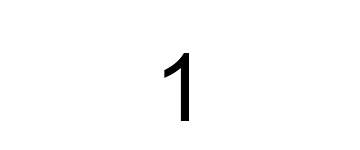
\includegraphics[width=0.8cm]{c:/github/surveyReport2022/standaloneData/sets_1.png}} & T & D,SD &  & T & A & A & T & D,SD & D,SD & T & D,SD & D,SD & T & D,SD & A & T & D,SD & D & T & A &  & T & D,SD & D,SD & T &  & 4 & 1 & 9 & 2\\
\raisebox{-.28\height} {
\includegraphics[width=0.8cm]{c:/github/surveyReport2022/standaloneData/sets_2.png}} & D & A & T & D,SD & D,SD & T &  & A & T & D & D,SD & T & D,SD & D,SD & T & D,SD & D,SD & T & D,SD & A & T & D,SD & D,SD & T & D,SD &  & 3 & 2 & 8 & 1\\
\raisebox{-.28\height} {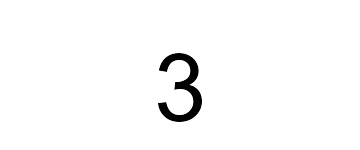
\includegraphics[width=0.8cm]{c:/github/surveyReport2022/standaloneData/sets_3.png}} & A &  & A & D,SD &  & D,SD &  & T & D,SD &  & T & D,SD & A & T & D,SD & A & T &  &  & T & A & A & T & A & A &  & 8 & 0 & 6 & 6\\
\raisebox{-.28\height} {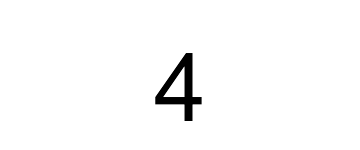
\includegraphics[width=0.8cm]{c:/github/surveyReport2022/standaloneData/sets_4.png}} & T & D,SD & A & T & D,SD & D,SD & T &  & A & T & D,SD & D,SD & T & D,SD & D,SD & T & D,SD & D,SD & D,SD &  & D,SD & D,SD & D,SD & D,SD & D,SD &  & 2 & 0 & 6 & 2\\
\raisebox{-.28\height} {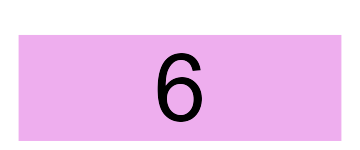
\includegraphics[width=0.8cm]{c:/github/surveyReport2022/standaloneData/sets_6.png}} & D,SD & T & D,SD & A & T & D,SD & D,SD & T & D,SD & D,SD & D,SD & D,SD & A &  & D,SD & A & T & D,F & A & T & D,SD & A & T & D,SD & T & D,SD & 5 & 1 & 7 & 0\\
\raisebox{-.28\height} {
\includegraphics[width=0.8cm]{c:/github/surveyReport2022/standaloneData/sets_7.png}} & T & D,SD & A & T & D,SD & D,SD & T & D,SD & A & T & D,SD & D,SD & T & D,SD & D,F & T & D,SD & A,F & T & D,SD & D,SD & D,SD & D,SD & D,SD & D,F &  & 3 & 2 & 7 & 0\\
\raisebox{-.28\height} {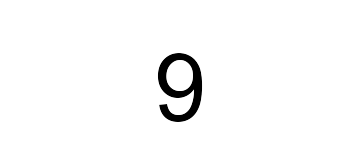
\includegraphics[width=0.8cm]{c:/github/surveyReport2022/standaloneData/sets_9.png}} & A & T & D,SD & A & T & D,SD & A & T & D,SD & D,SD & T & D,SD & D,SD & T & D,SD & D,SD & T & D,SD & D,SD & T & D,SD & D,SD & T & T,SD & D,SD &  & 3 & 0 & 8 & 0\\
\raisebox{-.28\height} {
\includegraphics[width=0.8cm]{c:/github/surveyReport2022/standaloneData/sets_10.png}} & T & D,SD & A & D,SD & D,SD & D,SD & T & T,SD & D,SD & T & D,SD & D,SD & D,SD & D,SD & D,SD & D,SD & D,SD & A & D,SD & D,SD & D,SD & D,SD & D,SD & T,SD & D,SD &  & 2 & 0 & 3 & 0\\
\raisebox{-.28\height} {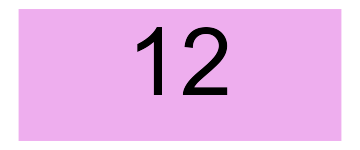
\includegraphics[width=0.8cm]{c:/github/surveyReport2022/standaloneData/sets_12.png}} & D,SD & T & D,SD & A & D,SD & D,SD & D,SD & T & D,SD & D,SD & D,SD & T,SD & D,SD &  & D,SD & D,SD & D,SD & D,SD & D,SD & D,SD & D,SD & A & D,SD & D,SD & D,SD & D,SD & 2 & 0 & 2 & 0\\
\raisebox{-.28\height} {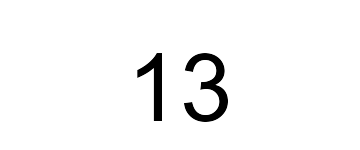
\includegraphics[width=0.8cm]{c:/github/surveyReport2022/standaloneData/sets_13.png}} & T & D,SD & A & T & D,SD & A & D,F & D,SD & D,SD & D,SD & D,SD & D,SD & D,SD & D,SD & D,SD & D,SD & D,SD & D,SD & D,SD & D,SD & D,SD & D,SD & D,SD & D,SD & D,SD &  & 2 & 1 & 2 & 0\\
\raisebox{-.28\height} {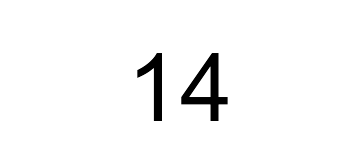
\includegraphics[width=0.8cm]{c:/github/surveyReport2022/standaloneData/sets_14.png}} & D,SD & D,SD & T & D,SD & A & D,SD & D,F & D,SD & T & D,SD & D,SD & D,SD & D,SD & D,SD & D,SD & D,SD & A & D,F & D,SD & D,SD & D,SD & D,SD &  & D,SD & D,SD &  & 2 & 2 & 2 & 1\\
\raisebox{-.28\height} {
\includegraphics[width=0.8cm]{c:/github/surveyReport2022/standaloneData/sets_15.png}} & D,F & T,F & D,SD & A,F & T,F & D,F & D,F & T,F & D,SD & D,SD & T,F & D,SD & D,SD & D,SD & D,SD & A,F & D,F & D,SD & D,SD & D,F & D,SD & D,SD & D,SD & D,SD & D,F &  & 2 & 6 & 4 & 0\\
\raisebox{-.28\height} {\includegraphics[width=0.8cm]{c:/github/surveyReport2022/standaloneData/sets_17.png}} & A & A & T & T,SD & D,F & T & D,SD & T,SD & T & T,SD & D,SD & D,SD & D,SD & D,SD & T & T,SD & T & D,SD & T,SD & D,SD & T,SD & D,SD & T,SD & D,SD & T,SD &  & 2 & 1 & 5 & 0\\
\raisebox{-.28\height} {\includegraphics[width=0.8cm]{c:/github/surveyReport2022/standaloneData/sets_19.png}} & T & D,SD & A & T & D,SD & A & T,F & D,SD & D,SD & T &  & D,SD & T,F &  & A,F & D,SD & T,SD & A & D,SD &  & D,SD & D,SD & T,SD &  & D,SD & D,SD & 4 & 0 & 5 & 3\\
\raisebox{-.28\height} {\includegraphics[width=0.8cm]{c:/github/surveyReport2022/standaloneData/sets_20.png}} & D,SD & T & T & D,SD &  & T &  & D,SD & T & D,SD & A & T & D,SD &  & T & D,SD & D,SD & T &  & D,SD & T &  & D,SD & T &  &  & 1 & 0 & 9 & 6\\
\raisebox{-.28\height} {\includegraphics[width=0.8cm]{c:/github/surveyReport2022/standaloneData/sets_22.png}} & T & D,SD & D,SD & T & D,SD & A & D,SD & D,SD & D,SD & T & T,SD & D,SD & D,SD & D,SD & A & D,SD & D,SD & D,SD & D,SD & D,SD & T & D,SD & D,SD & D,F & T,SD &  & 2 & 1 & 4 & 0\\
\raisebox{-.28\height} {\includegraphics[width=0.8cm]{c:/github/surveyReport2022/standaloneData/sets_23.png}} & D,F & T,SD &  & D,SD & T & T & D,SD & D,SD & T &  & D & D,SD &  &  &  &  & A & T & D,SD & D,SD & D,SD & D,SD & D,SD & D,SD & D,SD &  & 1 & 2 & 4 & 6\\
\raisebox{-.28\height} {\includegraphics[width=0.8cm]{c:/github/surveyReport2022/standaloneData/sets_24.png}} & A & T & T & D,SD & T & D,SD & A & T & D,SD & D,SD & T & D,SD & A & T & D & A & T & D & A & T & A & A & T & D,SD & A &  & 8 & 2 & 9 & 0\\
\raisebox{-.28\height} {\includegraphics[width=0.8cm]{c:/github/surveyReport2022/standaloneData/sets_25.png}} & T,F & D & A & T & D,SD & D,SD & T & D,SD & D,F & D,SD & T,F & A,F & T & D,SD & D,SD & D,SD & T,F & D,SD & T,F & D,F & D,SD & D,SD & D,SD & D,SD & D,F &  & 2 & 4 & 7 & 0\\
\raisebox{-.28\height} {\includegraphics[width=0.8cm]{c:/github/surveyReport2022/standaloneData/sets_26.png}} & D,SD & A & T &  & T,SD & T & D,SD & D,SD & T & D,SD & D,SD & D,SD & D,SD & A & T & D,SD & D,SD & T & D,SD & A & T & D,SD & D,SD & D,SD & D,SD &  & 3 & 0 & 6 & 1\\
\raisebox{-.28\height} {\includegraphics[width=0.8cm]{c:/github/surveyReport2022/standaloneData/sets_27.png}} & D,SD & T & D,SD & A & T & D,SD & T,SD & D,SD & D,SD & D,SD & T & D,SD & D,SD & T & D,SD & A & D,SD & D,SD & D,SD & D,SD & D,SD & D,SD & T,SD & D,SD & D,SD &  & 2 & 0 & 4 & 0\\
\raisebox{-.28\height} {\includegraphics[width=0.8cm]{c:/github/surveyReport2022/standaloneData/sets_28.png}} & T & D,SD & A & T & D,SD & D,SD & T & D,SD & D,SD & D,SD & D,SD & D,SD & T & D,SD & A & T & D,SD & D,SD & D,SD & D,SD & D,SD & D,SD & D,SD & T,SD & D,SD &  & 2 & 0 & 5 & 0\\
\raisebox{-.28\height} {\includegraphics[width=0.8cm]{c:/github/surveyReport2022/standaloneData/sets_29.png}} & D,SD & A,F & T & D,SD & D,SD & T & D,SD & D,SD & T & T,SD & D,SD & T & D,SD & D,SD & T & D,SD & A & D,SD & D,SD & D,SD & D,SD & D,SD & D,SD & D,SD & D,SD &  & 2 & 0 & 5 & 0\\
\raisebox{-.28\height} {\includegraphics[width=0.8cm]{c:/github/surveyReport2022/standaloneData/sets_31.png}} & T & D,SD & A & T & D,SD & D,SD & T & D,SD & A & T & D,SD & D,SD & T &  & A & T & D,SD & D,SD & D,SD & D,SD & D,SD & D,SD & D,SD & D,SD & D,SD & D,SD & 3 & 0 & 6 & 0\\
\raisebox{-.28\height} {\includegraphics[width=0.8cm]{c:/github/surveyReport2022/standaloneData/sets_33.png}} & A & T,F & D,F & A & T,F & D,F & D,F & T & D,SD & A,F & T,F & D,F & T,F & T,F & D,F & D,F & T,F & D,F & D,F & T & D,F & D,SD & T & D,F &  &  & 3 & 10 & 9 & 1\\
\raisebox{-.28\height} {\includegraphics[width=0.8cm]{c:/github/surveyReport2022/standaloneData/sets_34.png}} & T & D,SD & A & T & A & D,SD & T & D,SD & A &  &  & A & T & A & D,SD & T & D,SD & A & T & A & A & T & A & A & T &  & 10 & 0 & 8 & 2\\
\raisebox{-.28\height} {\includegraphics[width=0.8cm]{c:/github/surveyReport2022/standaloneData/sets_35.png}} & D,SD & A & T & D,SD & A &  & D & A & T & A & A & T & D,SD & A & T & A & D,SD & T & D & D,SD & T & D & D,SD & T & D,SD &  & 7 & 3 & 7 & 1\\
\raisebox{-.28\height} {\includegraphics[width=0.8cm]{c:/github/surveyReport2022/standaloneData/sets_36.png}} & A & T & D,SD &  & T & D,SD & A &  & D,SD & D,SD & T & D,SD & D,SD & T & D,SD & D,SD & T & D,SD & A & T & D,SD & A & T,F & D,SD & D,SD &  & 4 & 0 & 7 & 2\\
\raisebox{-.28\height} {\includegraphics[width=0.8cm]{c:/github/surveyReport2022/standaloneData/sets_37.png}} & T & D,SD & A & T & D,SD &  & T & D,SD & A & T & D,SD & A & T &  & A & T & D & A & T & D,SD & A & T & D,SD & A & T & D,SD & 7 & 1 & 9 & 1\\
\raisebox{-.28\height} {\includegraphics[width=0.8cm]{c:/github/surveyReport2022/standaloneData/sets_38.png}} & D,SD & A & T & D,SD & A & T & D,SD & D,SD & T & D,SD & D,SD & T & D,SD &  & T,F & D,SD & A & D,SD & D,SD & D,SD & D,F & D,SD & D,SD & D,SD & D,SD & D,SD & 3 & 1 & 5 & 0\\
\raisebox{-.28\height} {\includegraphics[width=0.8cm]{c:/github/surveyReport2022/standaloneData/sets_39.png}} &  &  & A & D,SD & T &  &  & T,F &  &  & A & T &  &  & A &  & A & A &  & A &  &  &  &  & A &  & 7 & 0 & 3 & 14\\
\raisebox{-.28\height} {\includegraphics[width=0.8cm]{c:/github/surveyReport2022/standaloneData/sets_40.png}} & D &  &  &  & A &  &  & A & A & T &  & A & T & A &  & T &  &  &  & A & A & T &  &  & T &  & 7 & 1 & 5 & 12\\
\raisebox{-.28\height} {\includegraphics[width=0.8cm]{c:/github/surveyReport2022/standaloneData/sets_41.png}} &  &  & T &  &  & T &  & A &  & D,SD & T & A &  & A &  &  &  & T &  &  &  & A &  &  &  &  & 4 & 0 & 4 & 16\\
\raisebox{-.28\height} {\includegraphics[width=0.8cm]{c:/github/surveyReport2022/standaloneData/sets_42.png}} &  & T &  & A & T & A & A,F &  & A & A & T &  &  & T & A & A &  & A & D & T &  & D &  &  &  &  & 8 & 2 & 5 & 10\\
\raisebox{-.28\height} {\includegraphics[width=0.8cm]{c:/github/surveyReport2022/standaloneData/sets_43.png}} &  &  & A & T & A & A & T & D,SD & A & T & D,SD & A & T &  & D,SD & T & D,SD & D,SD & T & D,SD & D,SD & T & D,SD & D,SD & T & D,SD & 5 & 0 & 8 & 2\\
\raisebox{-.28\height} {\includegraphics[width=0.8cm]{c:/github/surveyReport2022/standaloneData/sets_44.png}} & D,SD & D,SD & T & D,SD & A & T & D,SD & T,SD & T &  & D,SD & T & D,SD & D,SD & D,SD & D,SD & A & T & D,SD & D,SD & D,SD & D,SD & D,SD & D,SD & A & D & 3 & 1 & 5 & 0\\
\raisebox{-.28\height} {\includegraphics[width=0.8cm]{c:/github/surveyReport2022/standaloneData/sets_45.png}} & A & T & D & D,SD & T & D,SD & D,SD & A &  & T,SD & T & D,SD & T & T & D,SD &  & T & A & D,SD & T & A & T & D,SD & T & D,SD &  & 4 & 1 & 9 & 2\\
\raisebox{-.28\height} {\includegraphics[width=0.8cm]{c:/github/surveyReport2022/standaloneData/sets_46.png}} & T & D,SD & A & T & D,F & A & D,SD & D,SD & A & T &  & D,SD & T &  & A & T & D,SD & A & T & T,SD & A & T & D,SD & D,SD & T &  & 6 & 1 & 8 & 2\\
\raisebox{-.28\height} {\includegraphics[width=0.8cm]{c:/github/surveyReport2022/standaloneData/sets_47.png}} & D,SD & A & T & D,SD & D,SD & T & D,SD & A & T & D,SD & D,SD & T & D,SD & A & T & D,SD & D,SD & T & D,SD & A & T & D,SD & D,SD & D,SD & D,SD &  & 4 & 0 & 7 & 0\\
\raisebox{-.28\height} {\includegraphics[width=0.8cm]{c:/github/surveyReport2022/standaloneData/sets_48.png}} & A & T & D,SD & A & T & D,SD & D,SD & T & D,SD & D,SD & T & D,SD & A & T & D,SD & D,SD & T & D,SD & T,SD & T & D,SD & A & D,SD & D & D,SD &  & 4 & 1 & 7 & 0\\
\raisebox{-.28\height} {\includegraphics[width=0.8cm]{c:/github/surveyReport2022/standaloneData/sets_49.png}} & T & D,SD & A & T & D,SD & D,SD & T & D,SD & D,SD & T & D,SD & D,SD & T & D,SD & T & T & D & D,SD & D,SD & D,SD & D,SD & D,SD & D,SD & D,SD & D,SD &  & 1 & 1 & 7 & 0\\
\raisebox{-.28\height} {\includegraphics[width=0.8cm]{c:/github/surveyReport2022/standaloneData/sets_50.png}} & D,SD & A & T & D,SD & D & D,F & D,SD & D,SD & T & D,SD & D,SD & T,SD & T,SD & D,SD & T,SD & D,SD & T,SD & D,SD & D,SD & A & T,SD & D,SD & D,SD & D,SD & T,SD &  & 2 & 2 & 2 & 0\\
\raisebox{-.28\height} {\includegraphics[width=0.8cm]{c:/github/surveyReport2022/standaloneData/sets_51.png}} & A & T & D,SD & D,SD & T & D,SD & D,SD & D,SD & D,SD & D,SD & T & D,SD & A & D,SD & D,SD & D,SD & T & D,SD & D,SD & D,SD & D,SD & D,SD & D,SD & D,SD & D,SD &  & 2 & 0 & 4 & 0\\
\raisebox{-.28\height} {\includegraphics[width=0.8cm]{c:/github/surveyReport2022/standaloneData/sets_52.png}} & T & D,SD & A & T & D,SD & A & T & D & D & T & D,SD & D,SD & T & D,SD & D,SD & T & T,SD & A & T & D,SD & A & T & D,SD & T & T &  & 4 & 2 & 10 & 0\\
\raisebox{-.28\height} {\includegraphics[width=0.8cm]{c:/github/surveyReport2022/standaloneData/sets_53.png}} & D & A & T &  & A &  & A &  & T & A & A & T &  & A & T & A & A &  & A & A & T &  & D & T & D,SD &  & 10 & 2 & 6 & 6\\
\raisebox{-.28\height} {\includegraphics[width=0.8cm]{c:/github/surveyReport2022/standaloneData/sets_54.png}} & A & T & D,SD & A & T &  & A & T & D & A & T & D,SD & A & T & D,SD & A & T &  & A & T & D,SD & A & T & D &  &  & 8 & 2 & 8 & 3\\
\raisebox{-.28\height} {\includegraphics[width=0.8cm]{c:/github/surveyReport2022/standaloneData/sets_55.png}} & T & D,SD & A & T &  & D,SD & T & D,SD & D,SD & D,SD & D,SD & D,SD & T & D,SD & A & D,SD & D,SD & D,SD & T & D,SD & D,SD & D,SD & D,SD & D,SD & D,SD &  & 2 & 0 & 5 & 1\\
\raisebox{-.28\height} {\includegraphics[width=0.8cm]{c:/github/surveyReport2022/standaloneData/sets_56.png}} & D,SD & A & T & D,SD & A & T & D,SD & D,SD & T & D,SD & D,SD & T & D,SD & A & T & D,SD & D,SD & T & D,SD & A & T & D,SD & D,SD & T & D,SD &  & 4 & 0 & 8 & 0\\
\raisebox{-.28\height} {\includegraphics[width=0.8cm]{c:/github/surveyReport2022/standaloneData/sets_57.png}} & A & T & D,SD & D,SD & D,SD & D,SD & T,SD & T & D,SD & D,SD & D,SD & D,SD & T & T & D,SD & T,SD & T & D,SD & D,SD & T & D,SD & A & D,SD & D,SD & T,SD &  & 2 & 0 & 6 & 0\\
\raisebox{-.28\height} {\includegraphics[width=0.8cm]{c:/github/surveyReport2022/standaloneData/sets_58.png}} &  &  &  &  & A & A &  &  & A &  & A & A & T &  &  &  &  &  & T &  &  &  &  & A &  &  & 6 & 0 & 2 & 17\\
\raisebox{-.28\height} {\includegraphics[width=0.8cm]{c:/github/surveyReport2022/standaloneData/sets_59.png}} & D & A & T & D,SD & A & T & D,SD & A & T & D & A & T & D,SD &  & T & A & A & T & A & A & T & D,SD & A &  & D &  & 9 & 3 & 7 & 2\\
\raisebox{-.28\height} {\includegraphics[width=0.8cm]{c:/github/surveyReport2022/standaloneData/sets_60.png}} & A & T & D & D,SD & T & D & A & T & D &  & T & D & D & T &  &  &  & A &  &  &  &  &  &  &  &  & 3 & 5 & 5 & 11\\
\raisebox{-.28\height} {\includegraphics[width=0.8cm]{c:/github/surveyReport2022/standaloneData/sets_61.png}} & T & D,SD & A & T & D & D,SD & T & D,SD & D,SD & T & D,SD & D,SD & D,SD & D,SD & A & D,SD & D,SD & D,SD & T & D,F & D,SD & D,SD & D,F & D,F & D,SD &  & 2 & 4 & 5 & 0\\
\raisebox{-.28\height} {\includegraphics[width=0.8cm]{c:/github/surveyReport2022/standaloneData/sets_62.png}} &  &  & T & A & A & T & D & A &  & D,SD & D,SD & T & D,SD & D,SD & T & D,SD & A & T & D,SD & A & T & D,SD & D,SD & T & D &  & 5 & 2 & 7 & 3\\
\raisebox{-.28\height} {\includegraphics[width=0.8cm]{c:/github/surveyReport2022/standaloneData/sets_63.png}} & A,F & T & D,SD & D,SD & T & D,SD & A,F & D,SD & D,SD & D,SD & T & D,SD & D,SD & D,SD & D,SD & D,SD & T & D,SD & A & D,SD & D,SD & D,SD & D,SD & D,SD & D,SD &  & 3 & 0 & 4 & 0\\
\raisebox{-.28\height} {\includegraphics[width=0.8cm]{c:/github/surveyReport2022/standaloneData/sets_65.png}} & D,SD & A & T & D,SD & D,SD & T & D,SD & D,SD & T & D,SD & D,SD & T & D,SD & D,SD & D,SD & D,SD & A & D,SD & D,SD & D,SD & D,SD & D,SD & D,SD & D,SD & D,F &  & 2 & 1 & 4 & 0\\
\raisebox{-.28\height} {\includegraphics[width=0.8cm]{c:/github/surveyReport2022/standaloneData/sets_66.png}} & A & T & D,SD & D,SD & D,SD & D,SD & T,SD & T & D,SD & D,SD & D,SD & D,SD & D,SD & T & D,SD & A & D,SD & D,SD & D,SD & D,SD & D,SD & D,SD & D,SD & D,SD & D,SD &  & 2 & 0 & 3 & 0\\
\raisebox{-.28\height} {\includegraphics[width=0.8cm]{c:/github/surveyReport2022/standaloneData/sets_67.png}} & T & D,SD & A & T & D,SD & A & T & D,SD & D,SD & T & T,SD & A & T & D,SD & A & T & D,SD & A & T & D,SD & D,SD & D,SD & D,SD & D & D,SD &  & 5 & 1 & 7 & 0\\
\raisebox{-.28\height} {\includegraphics[width=0.8cm]{c:/github/surveyReport2022/standaloneData/sets_68.png}} &  & A & T & D,SD & D,SD & T & D,SD & D,SD & T & T & D,SD & T & D,SD & A & T & D,SD & D,SD & T & D,SD & D,SD & T & D,SD & D,SD & D,SD & D,SD &  & 2 & 0 & 8 & 1\\
\raisebox{-.28\height} {\includegraphics[width=0.8cm]{c:/github/surveyReport2022/standaloneData/sets_70.png}} & T & D,SD & A & T & D,SD & D & T & D,SD & T,SD & T & D,SD & D,SD & D,SD &  & A & D,SD &  &  & T & T,SD & A & T & D,SD &  & D,SD & D,SD & 3 & 1 & 6 & 3\\
\raisebox{-.28\height} {\includegraphics[width=0.8cm]{c:/github/surveyReport2022/standaloneData/sets_71.png}} & D & A & T & A & A & T & A & A & T & A &  & T &  & A & T & A & A & T & A & A & T & A & A & T &  &  & 13 & 1 & 8 & 3\\
\raisebox{-.28\height} {\includegraphics[width=0.8cm]{c:/github/surveyReport2022/standaloneData/sets_72.png}} & A & T & D,SD & D,SD & T & D & D & T & D & T,SD & T & D,SD & A & T & D & A & T & D,SD & A & T & D,SD & D,SD & T & D,SD & D &  & 4 & 5 & 8 & 0\\
\raisebox{-.28\height} {\includegraphics[width=0.8cm]{c:/github/surveyReport2022/standaloneData/sets_73.png}} & T & D,SD & A & T & D,SD & T,SD & T & D,SD & D,SD & D,SD & D,SD & D,SD & D,SD & D,SD & D,SD & D,SD & D & D,SD & D,SD & D,SD & D,SD & D,SD & D,SD & D,SD & D,SD &  & 1 & 1 & 3 & 0\\
\raisebox{-.28\height} {\includegraphics[width=0.8cm]{c:/github/surveyReport2022/standaloneData/sets_74.png}} & D,SD & D,SD & T & D,SD & A & T & D,SD & D,SD & D,SD & D,SD & D,SD & T,SD & D,SD & D,SD & D,SD & D,SD & A & T & D,SD & D,SD & D,SD & D,SD & D,SD & D,SD & D,SD &  & 2 & 0 & 3 & 0\\
\raisebox{-.28\height} {\includegraphics[width=0.8cm]{c:/github/surveyReport2022/standaloneData/sets_75.png}} & A & T & D & A & T &  & D,SD & T & D,SD & A & T & D,SD &  &  &  &  &  &  & A & T &  &  &  & A &  &  & 5 & 1 & 5 & 11\\
\raisebox{-.28\height} {\includegraphics[width=0.8cm]{c:/github/surveyReport2022/standaloneData/sets_76.png}} & T & D,SD & D,SD & T,SD & D,SD & A & D,SD & D,SD & D,SD & D,SD & D,SD & D,SD & T &  & A & D,SD & D,SD & D,SD & D,SD & D,SD &  & D,SD & D,SD & D,SD & D,SD & D,SD & 2 & 0 & 2 & 1\\
\raisebox{-.28\height} {\includegraphics[width=0.8cm]{c:/github/surveyReport2022/standaloneData/sets_77.png}} & D,SD & A & T & T,SD & T,SD & D,SD & D,SD & D,SD & T,SD & T,SD & D,SD & D,SD & T,SD & D,SD & T & D,SD & A & T & D,SD & D,SD & D,SD & D,SD & T,SD & T,SD & D,SD &  & 2 & 0 & 3 & 0\\
\raisebox{-.28\height} {\includegraphics[width=0.8cm]{c:/github/surveyReport2022/standaloneData/sets_78.png}} & A & T & A & A & T & D,SD & A & T & D,SD & A & T & D,SD & D,SD & T &  & A & T & D &  & T & D,SD &  & T & A & D,SD &  & 7 & 1 & 8 & 3\\
\raisebox{-.28\height} {\includegraphics[width=0.8cm]{c:/github/surveyReport2022/standaloneData/sets_79.png}} & D,SD & T & A & T & D,SD & D,SD & T & D,SD & D,SD &  & D,SD & A & T & D,SD & D,SD & T & D,SD & A & T &  & T,SD & D,SD &  & D,SD & D,SD &  & 3 & 0 & 6 & 3\\
\raisebox{-.28\height} {\includegraphics[width=0.8cm]{c:/github/surveyReport2022/standaloneData/sets_80.png}} & D,SD & D,SD & T & D,SD & A & T & D,SD & D,SD & T & D,SD & D,SD & T & D,SD & A & D,SD & D,SD & D,SD & T & D,SD & D,SD & D,SD & D,SD & A & D,SD & D,SD &  & 3 & 0 & 5 & 0\\
\raisebox{-.28\height} {\includegraphics[width=0.8cm]{c:/github/surveyReport2022/standaloneData/sets_81.png}} & T & T & D,SD & A & T & D,SD & A & T & D,SD & T &  & D,SD & A & T & D,SD & D,SD & T & D,SD & D,SD & T & D,SD &  & T & D,SD & D,SD &  & 3 & 0 & 9 & 2\\
\raisebox{-.28\height} {\includegraphics[width=0.8cm]{c:/github/surveyReport2022/standaloneData/sets_82.png}} &  &  &  &  &  & A &  &  &  &  & A &  &  &  &  &  &  &  &  &  &  &  &  &  &  &  & 2 & 0 & 0 & 23\\
\raisebox{-.28\height} {\includegraphics[width=0.8cm]{c:/github/surveyReport2022/standaloneData/sets_83.png}} & D,SD & A & T & D,SD & D,SD & T & D,SD & D,SD & T & D,SD & D,SD & T & D,SD &  & D,SD & D,SD & A & D,SD & D,SD & D,SD & D,SD & D,SD & D,SD & D,SD & D,SD & D,SD & 2 & 0 & 4 & 0\\
\raisebox{-.28\height} {\includegraphics[width=0.8cm]{c:/github/surveyReport2022/standaloneData/sets_84.png}} & A & T & D,SD & D,SD & T & D,SD & D,SD & D,SD & D,SD & D,SD & T & D,SD & A &  & D,SD & D,SD & T & D,SD & D,SD & T & D,SD & T,SD & T & T,SD & D,SD & D,SD & 2 & 0 & 6 & 0\\
\raisebox{-.28\height} {\includegraphics[width=0.8cm]{c:/github/surveyReport2022/standaloneData/sets_85.png}} &  &  & A &  & A &  & T & A & A &  & A & A & T & A & D,SD &  & T & D,SD &  & T & T &  &  &  & T &  & 7 & 0 & 6 & 10\\
\raisebox{-.28\height} {\includegraphics[width=0.8cm]{c:/github/surveyReport2022/standaloneData/sets_86.png}} & A & D,SD & T & D,SD &  & T &  &  & T & A &  & T &  & A &  & A & A & T &  &  & A & A & A & A & A &  & 10 & 0 & 5 & 8\\
\raisebox{-.28\height} {\includegraphics[width=0.8cm]{c:/github/surveyReport2022/standaloneData/sets_87.png}} & A & T & D,SD & A & T & D,SD & D,SD & T & D,SD & A & T & D,SD & D,SD & T & D,SD & D,SD & T & D,SD & D,SD & D,SD & D,SD & A & D,SD & D,SD & D,SD &  & 4 & 0 & 6 & 0\\
\raisebox{-.28\height} {\includegraphics[width=0.8cm]{c:/github/surveyReport2022/standaloneData/sets_88.png}} & T & D,SD & A & D,SD & D,SD & D,SD & T & D,SD & D,SD & D,SD & D,SD & D,SD & T & D,SD & D,SD & D,SD & D,SD & A & T & D,SD & D,SD & T & D,SD & D,SD & D,SD &  & 2 & 0 & 5 & 0\\
\raisebox{-.28\height} {\includegraphics[width=0.8cm]{c:/github/surveyReport2022/standaloneData/sets_89.png}} & D & A & T &  &  & T &  &  &  & A &  & T &  &  & T &  &  & T &  &  & T &  &  &  &  &  & 2 & 1 & 6 & 16\\
\raisebox{-.28\height} {\includegraphics[width=0.8cm]{c:/github/surveyReport2022/standaloneData/sets_90.png}} & A & T & D,SD & D,SD & T & D,SD & D,SD & D,SD & D,SD & D,SD & T & D,SD &  & D,SD & D,SD & A & T & D,SD & D,SD & D,SD & D,SD & D,SD & D,SD & D,SD & D,SD & D,SD & 2 & 0 & 4 & 0\\
\raisebox{-.28\height} {\includegraphics[width=0.8cm]{c:/github/surveyReport2022/standaloneData/sets_91.png}} & D & A &  & T & D,SD & A &  & D,SD &  & T &  &  & T &  &  & T &  &  &  &  & A &  &  & A & T & A & 5 & 1 & 5 & 12\\*
\end{longtable}
\endgroup{}
\end{landscape}
\clearpage

\clearpage

\section{SUMMARY OF SABLEFISH BIOLOGICAL DATA 2022.}
\label{app:fourth-appendix}

Summary of biological data collected for Sablefish by set, catch weight in kilograms and numbers of fish. Sablefish counts by trap are represented by sparklines, with every string picked up from the end location in 2021. Tagged fish counts are recorded by number of fish recovered and re-released, fish sampled and fish tagged and released. Tagged fish fork lengths are listed by count and mean (millimeters). Specimen counts are listed by sample type; mean fork lengths are tabulated. Standardized sets at mainland inlet localities are highlighted with green colour and StRS sets have no background colour. Those set numbers highlighted with purple colour had a camera deployed on the string of gear. The 4 sets highlighted in blue colour represent the 60 trap sets that were deployed to evaluate gear bottom-contact.
\begin{landscape}\begingroup\fontsize{8}{10}\selectfont
\begin{longtable}{>{\raggedleft\arraybackslash}p{0.3cm}>{\raggedleft\arraybackslash}p{0.6cm}>{\raggedleft\arraybackslash}p{0.7cm}>{\raggedleft\arraybackslash}p{1.4cm}>{\raggedleft\arraybackslash}p{0.9cm}>{\raggedleft\arraybackslash}p{1.3cm}>{\raggedleft\arraybackslash}p{0.9cm}>{\raggedleft\arraybackslash}p{1.5cm}>{\raggedleft\arraybackslash}p{0.9cm}>{\raggedleft\arraybackslash}p{0.7cm}>{\raggedleft\arraybackslash}p{0.6cm}>{\raggedleft\arraybackslash}p{0.7cm}>{\raggedleft\arraybackslash}p{0.8cm}>{\raggedleft\arraybackslash}p{0.6cm}>{\raggedleft\arraybackslash}p{0.6cm}>{\raggedleft\arraybackslash}p{1.1cm}>{\raggedleft\arraybackslash}p{0.7cm}>{\raggedleft\arraybackslash}p{0.7cm}}
\toprule
\multicolumn{1}{c}{\textbf{Set}} & \multicolumn{3}{c}{\textbf{Total Catch}} & \multicolumn{3}{c}{\textbf{Tagged Fish Counts}} & \multicolumn{2}{c}{\textbf{Tagged Fork Lengths(mm)}} & \multicolumn{6}{c}{\textbf{Specimen Count}} & \multicolumn{3}{c}{\textbf{Mean Fork Length(mm)}} \\
\cmidrule(l{3pt}r{3pt}){1-1} \cmidrule(l{3pt}r{3pt}){2-4} \cmidrule(l{3pt}r{3pt}){5-7} \cmidrule(l{3pt}r{3pt}){8-9} \cmidrule(l{3pt}r{3pt}){10-15} \cmidrule(l{3pt}r{3pt}){16-18}
\textbf{} & \textbf{kg} & \textbf{Count} & \textbf{Count by Trap} & \textbf{Recover-Rerelease} & \textbf{Tag Sample} & \textbf{Released} & \textbf{Count} & \textbf{Mean} & \textbf{Fork Length} & \textbf{Sex} & \textbf{Maturity} & \textbf{Otoliths} & \textbf{Weight} & \textbf{Count} & \textbf{Proportion Males} & \textbf{Males} & \textbf{Females}\\
\midrule
\endfirsthead
\multicolumn{18}{@{}l}{continued.}\\
\toprule
\multicolumn{1}{c}{\textbf{Set}} & \multicolumn{3}{c}{\textbf{Total Catch}} & \multicolumn{3}{c}{\textbf{Tagged Fish Counts}} & \multicolumn{2}{c}{\textbf{Tagged Fork Lengths(mm)}} & \multicolumn{6}{c}{\textbf{Specimen Count}} & \multicolumn{3}{c}{\textbf{Mean Fork Length(mm)}} \\
\cmidrule(l{3pt}r{3pt}){1-1} \cmidrule(l{3pt}r{3pt}){2-4} \cmidrule(l{3pt}r{3pt}){5-7} \cmidrule(l{3pt}r{3pt}){8-9} \cmidrule(l{3pt}r{3pt}){10-15} \cmidrule(l{3pt}r{3pt}){16-18}
\textbf{} & \textbf{kg} & \textbf{Count} & \textbf{Count by Trap} & \textbf{Recover-Rerelease} & \textbf{Tag Sample} & \textbf{Released} & \textbf{Count} & \textbf{Mean} & \textbf{Fork Length} & \textbf{Sex} & \textbf{Maturity} & \textbf{Otoliths} & \textbf{Weight} & \textbf{Count} & \textbf{Proportion Males} & \textbf{Males} & \textbf{Females}\\
\midrule
\endhead

\endfoot
\bottomrule
\endlastfoot
\raisebox{-.28\height} {\includegraphics[width=0.8cm]{c:/github/surveyReport2022/standaloneData/sets_1.png}} & 724 & 290 & \raisebox{.12\height} {\includegraphics[width=2cm]{c:/github/surveyReport2022/standaloneData/fig1.png}} & 0 & 0 & 109 & 109 & 609 & 49 & 48 & 48 & 48 & 48 & 49 & 0.35 & 575 & 617\\
\raisebox{-.28\height} {\includegraphics[width=0.8cm]{c:/github/surveyReport2022/standaloneData/sets_2.png}} & 915 & 434 & \raisebox{.12\height} {\includegraphics[width=2cm]{c:/github/surveyReport2022/standaloneData/fig2.png}} & 0 & 0 & 153 & 152 & 577 & 52 & 51 & 51 & 52 & 52 & 52 & 0.45 & 563 & 597\\
\raisebox{-.28\height} {\includegraphics[width=0.8cm]{c:/github/surveyReport2022/standaloneData/sets_3.png}} & 484 & 176 & \raisebox{.12\height} {\includegraphics[width=2cm]{c:/github/surveyReport2022/standaloneData/fig3.png}} & 0 & 0 & 52 & 52 & 625 & 52 & 52 & 52 & 52 & 52 & 52 & 0.21 & 627 & 632\\
\raisebox{-.28\height} {\includegraphics[width=0.8cm]{c:/github/surveyReport2022/standaloneData/sets_4.png}} & 930 & 543 & \raisebox{.12\height} {\includegraphics[width=2cm]{c:/github/surveyReport2022/standaloneData/fig4.png}} & 0 & 0 & 125 & 125 & 546 & 52 & 52 & 52 & 52 & 52 & 52 & 0.71 & 549 & 553\\
\raisebox{-.28\height} {\includegraphics[width=0.8cm]{c:/github/surveyReport2022/standaloneData/sets_5.png}} & 0 & 996 & \raisebox{.12\height} {\includegraphics[width=2cm]{c:/github/surveyReport2022/standaloneData/fig5.png}} & 0 & 0 & 0 & 0 & 0 & 2 & 2 & 2 & 2 & 2 & 2 & 1 & 575 & 0\\
\raisebox{-.28\height} {\includegraphics[width=0.8cm]{c:/github/surveyReport2022/standaloneData/sets_6.png}} & 699 & 428 & \raisebox{.12\height} {\includegraphics[width=2cm]{c:/github/surveyReport2022/standaloneData/fig6.png}} & 0 & 0 & 131 & 131 & 536 & 51 & 50 & 50 & 51 & 50 & 51 & 0.8 & 532 & 574\\
\raisebox{-.28\height} {\includegraphics[width=0.8cm]{c:/github/surveyReport2022/standaloneData/sets_7.png}} & 1105 & 520 & \raisebox{.12\height} {\includegraphics[width=2cm]{c:/github/surveyReport2022/standaloneData/fig7.png}} & 0 & 0 & 121 & 121 & 582 & 51 & 51 & 51 & 51 & 51 & 51 & 0.65 & 588 & 593\\
\raisebox{-.28\height} {\includegraphics[width=0.8cm]{c:/github/surveyReport2022/standaloneData/sets_8.png}} & 1608 & 818 & \raisebox{.12\height} {\includegraphics[width=2cm]{c:/github/surveyReport2022/standaloneData/fig8.png}} & 0 & 0 & 125 & 125 & 568 & 52 & 52 & 52 & 52 & 52 & 52 & 0.71 & 556 & 563\\
\raisebox{-.28\height} {\includegraphics[width=0.8cm]{c:/github/surveyReport2022/standaloneData/sets_9.png}} & 1170 & 503 & \raisebox{.12\height} {\includegraphics[width=2cm]{c:/github/surveyReport2022/standaloneData/fig9.png}} & 0 & 0 & 124 & 124 & 600 & 56 & 56 & 56 & 55 & 56 & 56 & 0.32 & 576 & 641\\
\raisebox{-.28\height} {\includegraphics[width=0.8cm]{c:/github/surveyReport2022/standaloneData/sets_10.png}} & 1249 & 741 & \raisebox{.12\height} {\includegraphics[width=2cm]{c:/github/surveyReport2022/standaloneData/fig10.png}} & 0 & 0 & 123 & 123 & 537 & 57 & 56 & 56 & 57 & 57 & 57 & 0.68 & 514 & 552\\
\raisebox{-.28\height} {\includegraphics[width=0.8cm]{c:/github/surveyReport2022/standaloneData/sets_11.png}} & 0 & 1780 & \raisebox{.12\height} {\includegraphics[width=2cm]{c:/github/surveyReport2022/standaloneData/fig11.png}} & 0 & 0 & 0 & 0 & 0 & 1 & 1 & 1 & 1 & 1 & 1 & 1 & 565 & 0\\
\raisebox{-.28\height} {\includegraphics[width=0.8cm]{c:/github/surveyReport2022/standaloneData/sets_12.png}} & 2296 & 1154 & \raisebox{.12\height} {\includegraphics[width=2cm]{c:/github/surveyReport2022/standaloneData/fig12.png}} & 0 & 0 & 121 & 121 & 565 & 55 & 53 & 53 & 54 & 55 & 55 & 0.38 & 559 & 602\\
\raisebox{-.28\height} {\includegraphics[width=0.8cm]{c:/github/surveyReport2022/standaloneData/sets_13.png}} & 2644 & 1390 & \raisebox{.12\height} {\includegraphics[width=2cm]{c:/github/surveyReport2022/standaloneData/fig13.png}} & 0 & 0 & 130 & 130 & 567 & 53 & 53 & 53 & 53 & 53 & 53 & 0.28 & 540 & 587\\
\raisebox{-.28\height} {\includegraphics[width=0.8cm]{c:/github/surveyReport2022/standaloneData/sets_14.png}} & 2673 & 1384 & \raisebox{.12\height} {\includegraphics[width=2cm]{c:/github/surveyReport2022/standaloneData/fig14.png}} & 0 & 0 & 153 & 153 & 561 & 54 & 53 & 53 & 53 & 53 & 54 & 0.47 & 549 & 589\\
\raisebox{-.28\height} {\includegraphics[width=0.8cm]{c:/github/surveyReport2022/standaloneData/sets_15.png}} & 3817 & 1957 & \raisebox{.12\height} {\includegraphics[width=2cm]{c:/github/surveyReport2022/standaloneData/fig15.png}} & 0 & 0 & 118 & 118 & 583 & 123 & 50 & 50 & 50 & 50 & 123 & 0.34 & 551 & 589\\
\raisebox{-.28\height} {\includegraphics[width=0.8cm]{c:/github/surveyReport2022/standaloneData/sets_16.png}} & 470 & 136 & \raisebox{.12\height} {\includegraphics[width=2cm]{c:/github/surveyReport2022/standaloneData/fig16.png}} & 0 & 0 & 47 & 47 & 667 & 50 & 50 & 50 & 50 & 50 & 50 & 0.06 & 653 & 663\\
\raisebox{-.28\height} {\includegraphics[width=0.8cm]{c:/github/surveyReport2022/standaloneData/sets_17.png}} & 1598 & 789 & \raisebox{.12\height} {\includegraphics[width=2cm]{c:/github/surveyReport2022/standaloneData/fig17.png}} & 0 & 0 & 153 & 153 & 563 & 54 & 54 & 54 & 54 & 54 & 54 & 0.5 & 528 & 596\\
\raisebox{-.28\height} {\includegraphics[width=0.8cm]{c:/github/surveyReport2022/standaloneData/sets_18.png}} & 0 & 1225 & \raisebox{.12\height} {\includegraphics[width=2cm]{c:/github/surveyReport2022/standaloneData/fig18.png}} & 0 & 0 & 0 & 0 & 0 & 3 & 4 & 4 & 3 & 3 & 4 & 0.5 & 545 & 585\\
\raisebox{-.28\height} {\includegraphics[width=0.8cm]{c:/github/surveyReport2022/standaloneData/sets_19.png}} & 684 & 471 & \raisebox{.12\height} {\includegraphics[width=2cm]{c:/github/surveyReport2022/standaloneData/fig19.png}} & 0 & 0 & 128 & 127 & 513 & 50 & 50 & 50 & 50 & 50 & 50 & 0.56 & 511 & 598\\
\raisebox{-.28\height} {\includegraphics[width=0.8cm]{c:/github/surveyReport2022/standaloneData/sets_20.png}} & 548 & 362 & \raisebox{.12\height} {\includegraphics[width=2cm]{c:/github/surveyReport2022/standaloneData/fig20.png}} & 0 & 0 & 113 & 113 & 525 & 50 & 50 & 50 & 50 & 50 & 50 & 0.66 & 512 & 575\\
\raisebox{-.28\height} {\includegraphics[width=0.8cm]{c:/github/surveyReport2022/standaloneData/sets_21.png}} & 0 & 1605 & \raisebox{.12\height} {\includegraphics[width=2cm]{c:/github/surveyReport2022/standaloneData/fig21.png}} & 0 & 0 & 0 & 0 & 0 & 7 & 8 & 8 & 6 & 8 & 8 & 0.75 & 607 & 633\\
\raisebox{-.28\height} {\includegraphics[width=0.8cm]{c:/github/surveyReport2022/standaloneData/sets_22.png}} & 1630 & 828 & \raisebox{.12\height} {\includegraphics[width=2cm]{c:/github/surveyReport2022/standaloneData/fig22.png}} & 0 & 0 & 123 & 123 & 577 & 53 & 51 & 51 & 51 & 51 & 53 & 0.65 & 546 & 602\\
\raisebox{-.28\height} {\includegraphics[width=0.8cm]{c:/github/surveyReport2022/standaloneData/sets_23.png}} & 1612 & 687 & \raisebox{.12\height} {\includegraphics[width=2cm]{c:/github/surveyReport2022/standaloneData/fig23.png}} & 0 & 0 & 146 & 146 & 606 & 54 & 54 & 54 & 54 & 54 & 54 & 0.15 & 593 & 601\\
\raisebox{-.28\height} {\includegraphics[width=0.8cm]{c:/github/surveyReport2022/standaloneData/sets_24.png}} & 618 & 214 & \raisebox{.12\height} {\includegraphics[width=2cm]{c:/github/surveyReport2022/standaloneData/fig24.png}} & 0 & 0 & 66 & 66 & 650 & 48 & 48 & 48 & 48 & 48 & 48 & 0.29 & 582 & 652\\
\raisebox{-.28\height} {\includegraphics[width=0.8cm]{c:/github/surveyReport2022/standaloneData/sets_25.png}} & 1226 & 535 & \raisebox{.12\height} {\includegraphics[width=2cm]{c:/github/surveyReport2022/standaloneData/fig25.png}} & 0 & 0 & 121 & 121 & 596 & 58 & 56 & 56 & 56 & 56 & 58 & 0.34 & 574 & 601\\
\raisebox{-.28\height} {\includegraphics[width=0.8cm]{c:/github/surveyReport2022/standaloneData/sets_26.png}} & 914 & 536 & \raisebox{.12\height} {\includegraphics[width=2cm]{c:/github/surveyReport2022/standaloneData/fig26.png}} & 0 & 0 & 154 & 154 & 530 & 51 & 51 & 51 & 51 & 51 & 51 & 0.82 & 534 & 565\\
\raisebox{-.28\height} {\includegraphics[width=0.8cm]{c:/github/surveyReport2022/standaloneData/sets_27.png}} & 2535 & 1024 & \raisebox{.12\height} {\includegraphics[width=2cm]{c:/github/surveyReport2022/standaloneData/fig27.png}} & 0 & 0 & 160 & 160 & 586 & 54 & 54 & 54 & 54 & 54 & 54 & 0.44 & 565 & 644\\
\raisebox{-.28\height} {\includegraphics[width=0.8cm]{c:/github/surveyReport2022/standaloneData/sets_28.png}} & 1260 & 663 & \raisebox{.12\height} {\includegraphics[width=2cm]{c:/github/surveyReport2022/standaloneData/fig28.png}} & 0 & 0 & 133 & 133 & 557 & 54 & 54 & 54 & 54 & 54 & 54 & 0.61 & 518 & 583\\
\raisebox{-.28\height} {\includegraphics[width=0.8cm]{c:/github/surveyReport2022/standaloneData/sets_29.png}} & 1352 & 719 & \raisebox{.12\height} {\includegraphics[width=2cm]{c:/github/surveyReport2022/standaloneData/fig29.png}} & 0 & 0 & 131 & 131 & 567 & 54 & 54 & 54 & 54 & 54 & 54 & 0.67 & 553 & 584\\
\raisebox{-.28\height} {\includegraphics[width=0.8cm]{c:/github/surveyReport2022/standaloneData/sets_30.png}} & 0 & 1307 & \raisebox{.12\height} {\includegraphics[width=2cm]{c:/github/surveyReport2022/standaloneData/fig30.png}} & 0 & 0 & 0 & 0 & 0 & 2 & 2 & 2 & 2 & 2 & 2 & 0.5 & 580 & 620\\
\raisebox{-.28\height} {\includegraphics[width=0.8cm]{c:/github/surveyReport2022/standaloneData/sets_31.png}} & 1029 & 509 & \raisebox{.12\height} {\includegraphics[width=2cm]{c:/github/surveyReport2022/standaloneData/fig31.png}} & 0 & 0 & 125 & 125 & 560 & 53 & 53 & 53 & 53 & 53 & 53 & 0.58 & 549 & 593\\
\raisebox{-.28\height} {\includegraphics[width=0.8cm]{c:/github/surveyReport2022/standaloneData/sets_32.png}} & 1395 & 665 & \raisebox{.12\height} {\includegraphics[width=2cm]{c:/github/surveyReport2022/standaloneData/fig32.png}} & 0 & 0 & 150 & 150 & 568 & 54 & 54 & 54 & 54 & 54 & 54 & 0.65 & 543 & 627\\
\raisebox{-.28\height} {\includegraphics[width=0.8cm]{c:/github/surveyReport2022/standaloneData/sets_33.png}} & 968 & 512 & \raisebox{.12\height} {\includegraphics[width=2cm]{c:/github/surveyReport2022/standaloneData/fig33.png}} & 0 & 0 & 108 & 108 & 584 & 61 & 52 & 52 & 52 & 52 & 61 & 0.23 & 577 & 620\\
\raisebox{-.28\height} {\includegraphics[width=0.8cm]{c:/github/surveyReport2022/standaloneData/sets_34.png}} & 352 & 126 & \raisebox{.12\height} {\includegraphics[width=2cm]{c:/github/surveyReport2022/standaloneData/fig34.png}} & 0 & 0 & 56 & 56 & 636 & 47 & 47 & 47 & 47 & 47 & 47 & 0.36 & 581 & 657\\
\raisebox{-.28\height} {\includegraphics[width=0.8cm]{c:/github/surveyReport2022/standaloneData/sets_35.png}} & 585 & 206 & \raisebox{.12\height} {\includegraphics[width=2cm]{c:/github/surveyReport2022/standaloneData/fig35.png}} & 0 & 0 & 47 & 47 & 618 & 54 & 54 & 54 & 54 & 54 & 54 & 0.26 & 593 & 637\\
\raisebox{-.28\height} {\includegraphics[width=0.8cm]{c:/github/surveyReport2022/standaloneData/sets_36.png}} & 814 & 387 & \raisebox{.12\height} {\includegraphics[width=2cm]{c:/github/surveyReport2022/standaloneData/fig36.png}} & 0 & 0 & 108 & 108 & 577 & 62 & 56 & 56 & 56 & 56 & 62 & 0.55 & 554 & 584\\
\raisebox{-.28\height} {\includegraphics[width=0.8cm]{c:/github/surveyReport2022/standaloneData/sets_37.png}} & 620 & 219 & \raisebox{.12\height} {\includegraphics[width=2cm]{c:/github/surveyReport2022/standaloneData/fig37.png}} & 0 & 0 & 69 & 69 & 637 & 55 & 55 & 55 & 55 & 55 & 55 & 0.25 & 586 & 673\\
\raisebox{-.28\height} {\includegraphics[width=0.8cm]{c:/github/surveyReport2022/standaloneData/sets_38.png}} & 1360 & 766 & \raisebox{.12\height} {\includegraphics[width=2cm]{c:/github/surveyReport2022/standaloneData/fig38.png}} & 0 & 0 & 153 & 152 & 554 & 59 & 59 & 59 & 59 & 59 & 59 & 0.76 & 541 & 564\\
\raisebox{-.28\height} {\includegraphics[width=0.8cm]{c:/github/surveyReport2022/standaloneData/sets_39.png}} & 168 & 58 & \raisebox{.12\height} {\includegraphics[width=2cm]{c:/github/surveyReport2022/standaloneData/fig39.png}} & 0 & 0 & 10 & 10 & 679 & 44 & 43 & 43 & 43 & 43 & 44 & 0.21 & 574 & 643\\
\raisebox{-.28\height} {\includegraphics[width=0.8cm]{c:/github/surveyReport2022/standaloneData/sets_40.png}} & 61 & 30 & \raisebox{.12\height} {\includegraphics[width=2cm]{c:/github/surveyReport2022/standaloneData/fig40.png}} & 0 & 0 & 14 & 14 & 563 & 15 & 15 & 15 & 15 & 15 & 15 & 0.47 & 554 & 640\\
\raisebox{-.28\height} {\includegraphics[width=0.8cm]{c:/github/surveyReport2022/standaloneData/sets_41.png}} & 352 & 132 & \raisebox{.12\height} {\includegraphics[width=2cm]{c:/github/surveyReport2022/standaloneData/fig41.png}} & 0 & 0 & 45 & 45 & 620 & 45 & 45 & 45 & 45 & 45 & 45 & 0.29 & 583 & 638\\
\raisebox{-.28\height} {\includegraphics[width=0.8cm]{c:/github/surveyReport2022/standaloneData/sets_42.png}} & 333 & 95 & \raisebox{.12\height} {\includegraphics[width=2cm]{c:/github/surveyReport2022/standaloneData/fig42.png}} & 0 & 0 & 15 & 15 & 680 & 51 & 48 & 48 & 48 & 48 & 51 & 0.46 & 665 & 673\\
\raisebox{-.28\height} {\includegraphics[width=0.8cm]{c:/github/surveyReport2022/standaloneData/sets_43.png}} & 649 & 260 & \raisebox{.12\height} {\includegraphics[width=2cm]{c:/github/surveyReport2022/standaloneData/fig43.png}} & 0 & 0 & 90 & 89 & 612 & 56 & 56 & 55 & 56 & 56 & 56 & 0.34 & 618 & 649\\
\raisebox{-.28\height} {\includegraphics[width=0.8cm]{c:/github/surveyReport2022/standaloneData/sets_44.png}} & 1190 & 517 & \raisebox{.12\height} {\includegraphics[width=2cm]{c:/github/surveyReport2022/standaloneData/fig44.png}} & 0 & 0 & 117 & 117 & 585 & 54 & 53 & 53 & 53 & 53 & 54 & 0.55 & 583 & 618\\
\raisebox{-.28\height} {\includegraphics[width=0.8cm]{c:/github/surveyReport2022/standaloneData/sets_45.png}} & 732 & 298 & \raisebox{.12\height} {\includegraphics[width=2cm]{c:/github/surveyReport2022/standaloneData/fig45.png}} & 0 & 0 & 96 & 96 & 609 & 72 & 72 & 72 & 72 & 72 & 72 & 0.54 & 583 & 612\\
\raisebox{-.28\height} {\includegraphics[width=0.8cm]{c:/github/surveyReport2022/standaloneData/sets_46.png}} & 729 & 262 & \raisebox{.12\height} {\includegraphics[width=2cm]{c:/github/surveyReport2022/standaloneData/fig46.png}} & 0 & 0 & 103 & 103 & 619 & 53 & 52 & 52 & 51 & 52 & 53 & 0.19 & 591 & 650\\
\raisebox{-.28\height} {\includegraphics[width=0.8cm]{c:/github/surveyReport2022/standaloneData/sets_47.png}} & 1091 & 412 & \raisebox{.12\height} {\includegraphics[width=2cm]{c:/github/surveyReport2022/standaloneData/fig47.png}} & 0 & 0 & 135 & 135 & 606 & 51 & 51 & 51 & 51 & 51 & 51 & 0.25 & 619 & 615\\
\raisebox{-.28\height} {\includegraphics[width=0.8cm]{c:/github/surveyReport2022/standaloneData/sets_48.png}} & 908 & 442 & \raisebox{.12\height} {\includegraphics[width=2cm]{c:/github/surveyReport2022/standaloneData/fig48.png}} & 0 & 0 & 124 & 123 & 570 & 53 & 53 & 53 & 53 & 53 & 53 & 0.66 & 564 & 618\\
\raisebox{-.28\height} {\includegraphics[width=0.8cm]{c:/github/surveyReport2022/standaloneData/sets_49.png}} & 1558 & 697 & \raisebox{.12\height} {\includegraphics[width=2cm]{c:/github/surveyReport2022/standaloneData/fig49.png}} & 0 & 0 & 136 & 135 & 589 & 51 & 51 & 51 & 51 & 51 & 51 & 0.61 & 573 & 617\\
\raisebox{-.28\height} {\includegraphics[width=0.8cm]{c:/github/surveyReport2022/standaloneData/sets_50.png}} & 2093 & 1445 & \raisebox{.12\height} {\includegraphics[width=2cm]{c:/github/surveyReport2022/standaloneData/fig50.png}} & 0 & 0 & 127 & 127 & 514 & 49 & 49 & 49 & 49 & 49 & 49 & 0.71 & 518 & 574\\
\raisebox{-.28\height} {\includegraphics[width=0.8cm]{c:/github/surveyReport2022/standaloneData/sets_51.png}} & 1851 & 848 & \raisebox{.12\height} {\includegraphics[width=2cm]{c:/github/surveyReport2022/standaloneData/fig51.png}} & 0 & 0 & 128 & 128 & 584 & 52 & 51 & 51 & 52 & 52 & 52 & 0.67 & 591 & 650\\
\raisebox{-.28\height} {\includegraphics[width=0.8cm]{c:/github/surveyReport2022/standaloneData/sets_52.png}} & 635 & 253 & \raisebox{.12\height} {\includegraphics[width=2cm]{c:/github/surveyReport2022/standaloneData/fig52.png}} & 0 & 0 & 79 & 79 & 601 & 53 & 53 & 53 & 53 & 53 & 53 & 0.38 & 582 & 601\\
\raisebox{-.28\height} {\includegraphics[width=0.8cm]{c:/github/surveyReport2022/standaloneData/sets_53.png}} & 248 & 84 & \raisebox{.12\height} {\includegraphics[width=2cm]{c:/github/surveyReport2022/standaloneData/fig53.png}} & 0 & 0 & 14 & 14 & 608 & 51 & 51 & 51 & 51 & 51 & 51 & 0.14 & 614 & 659\\
\raisebox{-.28\height} {\includegraphics[width=0.8cm]{c:/github/surveyReport2022/standaloneData/sets_54.png}} & 475 & 154 & \raisebox{.12\height} {\includegraphics[width=2cm]{c:/github/surveyReport2022/standaloneData/fig54.png}} & 0 & 0 & 53 & 51 & 635 & 53 & 53 & 53 & 53 & 53 & 53 & 0.06 & 578 & 648\\
\raisebox{-.28\height} {\includegraphics[width=0.8cm]{c:/github/surveyReport2022/standaloneData/sets_55.png}} & 1259 & 530 & \raisebox{.12\height} {\includegraphics[width=2cm]{c:/github/surveyReport2022/standaloneData/fig55.png}} & 0 & 0 & 129 & 129 & 586 & 53 & 53 & 53 & 53 & 53 & 53 & 0.49 & 591 & 628\\
\raisebox{-.28\height} {\includegraphics[width=0.8cm]{c:/github/surveyReport2022/standaloneData/sets_56.png}} & 1025 & 361 & \raisebox{.12\height} {\includegraphics[width=2cm]{c:/github/surveyReport2022/standaloneData/fig56.png}} & 0 & 0 & 119 & 119 & 646 & 52 & 52 & 52 & 52 & 52 & 52 & 0.6 & 604 & 696\\
\raisebox{-.28\height} {\includegraphics[width=0.8cm]{c:/github/surveyReport2022/standaloneData/sets_57.png}} & 1471 & 789 & \raisebox{.12\height} {\includegraphics[width=2cm]{c:/github/surveyReport2022/standaloneData/fig57.png}} & 0 & 0 & 135 & 135 & 567 & 52 & 52 & 52 & 52 & 52 & 52 & 0.81 & 555 & 590\\
\raisebox{-.28\height} {\includegraphics[width=0.8cm]{c:/github/surveyReport2022/standaloneData/sets_58.png}} & 116 & 37 & \raisebox{.12\height} {\includegraphics[width=2cm]{c:/github/surveyReport2022/standaloneData/fig58.png}} & 0 & 0 & 6 & 6 & 604 & 31 & 31 & 31 & 31 & 31 & 31 & 0.1 & 565 & 647\\
\raisebox{-.28\height} {\includegraphics[width=0.8cm]{c:/github/surveyReport2022/standaloneData/sets_59.png}} & 465 & 177 & \raisebox{.12\height} {\includegraphics[width=2cm]{c:/github/surveyReport2022/standaloneData/fig59.png}} & 0 & 0 & 58 & 58 & 643 & 51 & 51 & 51 & 51 & 51 & 51 & 0.55 & 608 & 661\\
\raisebox{-.28\height} {\includegraphics[width=0.8cm]{c:/github/surveyReport2022/standaloneData/sets_60.png}} & 332 & 105 & \raisebox{.12\height} {\includegraphics[width=2cm]{c:/github/surveyReport2022/standaloneData/fig60.png}} & 0 & 0 & 34 & 34 & 631 & 32 & 32 & 32 & 32 & 32 & 32 & 0.16 & 611 & 654\\
\raisebox{-.28\height} {\includegraphics[width=0.8cm]{c:/github/surveyReport2022/standaloneData/sets_61.png}} & 1352 & 650 & \raisebox{.12\height} {\includegraphics[width=2cm]{c:/github/surveyReport2022/standaloneData/fig61.png}} & 0 & 0 & 126 & 125 & 570 & 53 & 52 & 52 & 48 & 52 & 53 & 0.5 & 554 & 571\\
\raisebox{-.28\height} {\includegraphics[width=0.8cm]{c:/github/surveyReport2022/standaloneData/sets_62.png}} & 523 & 184 & \raisebox{.12\height} {\includegraphics[width=2cm]{c:/github/surveyReport2022/standaloneData/fig62.png}} & 0 & 0 & 32 & 32 & 649 & 52 & 52 & 52 & 52 & 52 & 52 & 0.44 & 600 & 693\\
\raisebox{-.28\height} {\includegraphics[width=0.8cm]{c:/github/surveyReport2022/standaloneData/sets_63.png}} & 1507 & 691 & \raisebox{.12\height} {\includegraphics[width=2cm]{c:/github/surveyReport2022/standaloneData/fig63.png}} & 0 & 0 & 133 & 133 & 576 & 65 & 64 & 64 & 64 & 64 & 65 & 0.3 & 566 & 593\\
\raisebox{-.28\height} {\includegraphics[width=0.8cm]{c:/github/surveyReport2022/standaloneData/sets_64.png}} & 0 & 753 & \raisebox{.12\height} {\includegraphics[width=2cm]{c:/github/surveyReport2022/standaloneData/fig64.png}} & 0 & 0 & 0 & 0 & 0 & 0 & 0 & 0 & 0 & 0 & 0 & 0 & 0 & 0\\
\raisebox{-.28\height} {\includegraphics[width=0.8cm]{c:/github/surveyReport2022/standaloneData/sets_65.png}} & 2054 & 1111 & \raisebox{.12\height} {\includegraphics[width=2cm]{c:/github/surveyReport2022/standaloneData/fig65.png}} & 0 & 0 & 143 & 143 & 547 & 56 & 56 & 56 & 56 & 56 & 56 & 0.45 & 553 & 574\\
\raisebox{-.28\height} {\includegraphics[width=0.8cm]{c:/github/surveyReport2022/standaloneData/sets_66.png}} & 2481 & 1260 & \raisebox{.12\height} {\includegraphics[width=2cm]{c:/github/surveyReport2022/standaloneData/fig66.png}} & 0 & 0 & 158 & 158 & 556 & 56 & 56 & 56 & 56 & 56 & 56 & 0.61 & 549 & 565\\
\raisebox{-.28\height} {\includegraphics[width=0.8cm]{c:/github/surveyReport2022/standaloneData/sets_67.png}} & 1304 & 406 & \raisebox{.12\height} {\includegraphics[width=2cm]{c:/github/surveyReport2022/standaloneData/fig67.png}} & 0 & 0 & 124 & 124 & 635 & 59 & 58 & 58 & 58 & 58 & 59 & 0.21 & 620 & 681\\
\raisebox{-.28\height} {\includegraphics[width=0.8cm]{c:/github/surveyReport2022/standaloneData/sets_68.png}} & 1397 & 482 & \raisebox{.12\height} {\includegraphics[width=2cm]{c:/github/surveyReport2022/standaloneData/fig68.png}} & 0 & 0 & 123 & 122 & 621 & 51 & 51 & 51 & 51 & 51 & 51 & 0.27 & 592 & 659\\
\raisebox{-.28\height} {\includegraphics[width=0.8cm]{c:/github/surveyReport2022/standaloneData/sets_69.png}} & 794 & 326 & \raisebox{.12\height} {\includegraphics[width=2cm]{c:/github/surveyReport2022/standaloneData/fig69.png}} & 0 & 0 & 89 & 89 & 619 & 51 & 51 & 51 & 51 & 51 & 51 & 0.49 & 592 & 631\\
\raisebox{-.28\height} {\includegraphics[width=0.8cm]{c:/github/surveyReport2022/standaloneData/sets_70.png}} & 828 & 401 & \raisebox{.12\height} {\includegraphics[width=2cm]{c:/github/surveyReport2022/standaloneData/fig70.png}} & 0 & 0 & 132 & 132 & 576 & 50 & 50 & 50 & 50 & 50 & 50 & 0.66 & 551 & 610\\
\raisebox{-.28\height} {\includegraphics[width=0.8cm]{c:/github/surveyReport2022/standaloneData/sets_71.png}} & 277 & 90 & \raisebox{.12\height} {\includegraphics[width=2cm]{c:/github/surveyReport2022/standaloneData/fig71.png}} & 0 & 0 & 42 & 42 & 632 & 44 & 44 & 44 & 44 & 44 & 44 & 0.34 & 643 & 682\\
\raisebox{-.28\height} {\includegraphics[width=0.8cm]{c:/github/surveyReport2022/standaloneData/sets_72.png}} & 1218 & 367 & \raisebox{.12\height} {\includegraphics[width=2cm]{c:/github/surveyReport2022/standaloneData/fig72.png}} & 0 & 0 & 123 & 122 & 654 & 53 & 53 & 53 & 53 & 53 & 53 & 0.45 & 613 & 674\\
\raisebox{-.28\height} {\includegraphics[width=0.8cm]{c:/github/surveyReport2022/standaloneData/sets_73.png}} & 2474 & 1154 & \raisebox{.12\height} {\includegraphics[width=2cm]{c:/github/surveyReport2022/standaloneData/fig73.png}} & 0 & 0 & 124 & 123 & 566 & 54 & 51 & 51 & 52 & 52 & 54 & 0.65 & 564 & 582\\
\raisebox{-.28\height} {\includegraphics[width=0.8cm]{c:/github/surveyReport2022/standaloneData/sets_74.png}} & 2371 & 1128 & \raisebox{.12\height} {\includegraphics[width=2cm]{c:/github/surveyReport2022/standaloneData/fig74.png}} & 0 & 0 & 179 & 178 & 572 & 51 & 51 & 51 & 51 & 51 & 51 & 0.57 & 575 & 610\\
\raisebox{-.28\height} {\includegraphics[width=0.8cm]{c:/github/surveyReport2022/standaloneData/sets_75.png}} & 365 & 120 & \raisebox{.12\height} {\includegraphics[width=2cm]{c:/github/surveyReport2022/standaloneData/fig75.png}} & 0 & 0 & 31 & 31 & 642 & 49 & 49 & 49 & 49 & 49 & 49 & 0.27 & 626 & 660\\
\raisebox{-.28\height} {\includegraphics[width=0.8cm]{c:/github/surveyReport2022/standaloneData/sets_76.png}} & 2218 & 1498 & \raisebox{.12\height} {\includegraphics[width=2cm]{c:/github/surveyReport2022/standaloneData/fig76.png}} & 0 & 0 & 174 & 174 & 522 & 52 & 52 & 52 & 52 & 52 & 52 & 0.71 & 506 & 564\\
\raisebox{-.28\height} {\includegraphics[width=0.8cm]{c:/github/surveyReport2022/standaloneData/sets_77.png}} & 1681 & 975 & \raisebox{.12\height} {\includegraphics[width=2cm]{c:/github/surveyReport2022/standaloneData/fig77.png}} & 0 & 0 & 143 & 143 & 544 & 49 & 49 & 49 & 49 & 49 & 49 & 0.88 & 524 & 566\\
\raisebox{-.28\height} {\includegraphics[width=0.8cm]{c:/github/surveyReport2022/standaloneData/sets_78.png}} & 543 & 216 & \raisebox{.12\height} {\includegraphics[width=2cm]{c:/github/surveyReport2022/standaloneData/fig78.png}} & 0 & 0 & 79 & 79 & 601 & 51 & 51 & 51 & 51 & 51 & 51 & 0.39 & 599 & 629\\
\raisebox{-.28\height} {\includegraphics[width=0.8cm]{c:/github/surveyReport2022/standaloneData/sets_79.png}} & 1289 & 485 & \raisebox{.12\height} {\includegraphics[width=2cm]{c:/github/surveyReport2022/standaloneData/fig79.png}} & 0 & 0 & 123 & 123 & 607 & 53 & 53 & 53 & 49 & 53 & 53 & 0.49 & 595 & 598\\
\raisebox{-.28\height} {\includegraphics[width=0.8cm]{c:/github/surveyReport2022/standaloneData/sets_80.png}} & 1539 & 721 & \raisebox{.12\height} {\includegraphics[width=2cm]{c:/github/surveyReport2022/standaloneData/fig80.png}} & 0 & 0 & 130 & 130 & 579 & 51 & 51 & 51 & 51 & 51 & 51 & 0.63 & 564 & 607\\
\raisebox{-.28\height} {\includegraphics[width=0.8cm]{c:/github/surveyReport2022/standaloneData/sets_81.png}} & 1044 & 497 & \raisebox{.12\height} {\includegraphics[width=2cm]{c:/github/surveyReport2022/standaloneData/fig81.png}} & 0 & 0 & 144 & 144 & 579 & 47 & 47 & 47 & 47 & 47 & 47 & 0.62 & 559 & 609\\
\raisebox{-.28\height} {\includegraphics[width=0.8cm]{c:/github/surveyReport2022/standaloneData/sets_82.png}} & 5 & 2 & \raisebox{.12\height} {\includegraphics[width=2cm]{c:/github/surveyReport2022/standaloneData/fig82.png}} & 0 & 0 & 0 & 0 & 0 & 2 & 2 & 2 & 2 & 2 & 2 & 0 & 0 & 620\\
\raisebox{-.28\height} {\includegraphics[width=0.8cm]{c:/github/surveyReport2022/standaloneData/sets_83.png}} & 1779 & 811 & \raisebox{.12\height} {\includegraphics[width=2cm]{c:/github/surveyReport2022/standaloneData/fig83.png}} & 0 & 0 & 121 & 121 & 571 & 53 & 53 & 53 & 53 & 53 & 53 & 0.62 & 567 & 582\\
\raisebox{-.28\height} {\includegraphics[width=0.8cm]{c:/github/surveyReport2022/standaloneData/sets_84.png}} & 1209 & 596 & \raisebox{.12\height} {\includegraphics[width=2cm]{c:/github/surveyReport2022/standaloneData/fig84.png}} & 0 & 0 & 124 & 124 & 580 & 52 & 52 & 52 & 52 & 52 & 52 & 0.65 & 540 & 581\\
\raisebox{-.28\height} {\includegraphics[width=0.8cm]{c:/github/surveyReport2022/standaloneData/sets_85.png}} & 275 & 111 & \raisebox{.12\height} {\includegraphics[width=2cm]{c:/github/surveyReport2022/standaloneData/fig85.png}} & 0 & 0 & 33 & 32 & 600 & 56 & 55 & 55 & 55 & 55 & 56 & 0.35 & 564 & 619\\
\raisebox{-.28\height} {\includegraphics[width=0.8cm]{c:/github/surveyReport2022/standaloneData/sets_86.png}} & 304 & 119 & \raisebox{.12\height} {\includegraphics[width=2cm]{c:/github/surveyReport2022/standaloneData/fig86.png}} & 0 & 0 & 47 & 47 & 602 & 41 & 40 & 40 & 40 & 40 & 41 & 0.45 & 578 & 620\\
\raisebox{-.28\height} {\includegraphics[width=0.8cm]{c:/github/surveyReport2022/standaloneData/sets_87.png}} & 1142 & 532 & \raisebox{.12\height} {\includegraphics[width=2cm]{c:/github/surveyReport2022/standaloneData/fig87.png}} & 0 & 0 & 123 & 123 & 598 & 50 & 50 & 50 & 50 & 50 & 50 & 0.78 & 556 & 647\\
\raisebox{-.28\height} {\includegraphics[width=0.8cm]{c:/github/surveyReport2022/standaloneData/sets_88.png}} & 1562 & 852 & \raisebox{.12\height} {\includegraphics[width=2cm]{c:/github/surveyReport2022/standaloneData/fig88.png}} & 0 & 0 & 141 & 141 & 561 & 55 & 55 & 55 & 55 & 55 & 55 & 0.71 & 538 & 588\\
\raisebox{-.28\height} {\includegraphics[width=0.8cm]{c:/github/surveyReport2022/standaloneData/sets_89.png}} & 95 & 19 & \raisebox{.12\height} {\includegraphics[width=2cm]{c:/github/surveyReport2022/standaloneData/fig89.png}} & 0 & 0 & 13 & 13 & 731 & 5 & 5 & 5 & 5 & 5 & 5 & 0 & 0 & 793\\
\raisebox{-.28\height} {\includegraphics[width=0.8cm]{c:/github/surveyReport2022/standaloneData/sets_90.png}} & 1704 & 783 & \raisebox{.12\height} {\includegraphics[width=2cm]{c:/github/surveyReport2022/standaloneData/fig90.png}} & 0 & 0 & 147 & 147 & 580 & 48 & 48 & 48 & 48 & 48 & 48 & 0.38 & 569 & 597\\
\raisebox{-.28\height} {\includegraphics[width=0.8cm]{c:/github/surveyReport2022/standaloneData/sets_91.png}} & 216 & 76 & \raisebox{.12\height} {\includegraphics[width=2cm]{c:/github/surveyReport2022/standaloneData/fig91.png}} & 0 & 0 & 32 & 32 & 629 & 33 & 33 & 33 & 33 & 33 & 33 & 0 & 0 & 635\\
\midrule
Movement &  & 3,619 &  & 0 & 0 & 0 & 567 &  & 224 & 222 & 222 & 222 & 222 & 224 &  &  & \\
Other &  & 49,388 &  & 0 & 0 & 8,209 & 8,195 &  & 4,139 & 4,029 & 4,028 &  & 4,034 & 4,141 &  &  & \\
\midrule
\textbf{Total} & \textbf{} & \textbf{53,007} & \textbf{} & \textbf{0} & \textbf{0} & \textbf{8,776} & \textbf{8,762} & \textbf{} & \textbf{4,363} & \textbf{4,251} & \textbf{4,250} & \textbf{4,244} & \textbf{4,256} & \textbf{4,365} & \textbf{} & \textbf{} & \textbf{}\\*
\end{longtable}
\endgroup{}
\end{landscape}
\clearpage

\section{SUMMARY OF BIOLOGICAL DATA FOR THE ROUGHEYE/BLACKSPOTTED ROCKFISH COMPLEX.}
\label{app:fifth-appendix}

Biological data collected for Rougheye/Blackspotted Rockfish complex. Each set is listed with counts of specimens sampled, calculations of mean fork lengths and the number of species visually identified as either a RE = Rougheye Rockfish, BS = Blackspotted Rockfish or a hybrid. All were captured on StRS sets. ~\\
\hspace*{0.333em}\\

\begingroup\fontsize{8}{10}\selectfont
\begin{longtable}{>{\raggedright\arraybackslash}p{0.5cm}>{\raggedright\arraybackslash}p{0.7cm}>{\raggedright\arraybackslash}p{0.7cm}>{\raggedright\arraybackslash}p{0.4cm}>{\raggedright\arraybackslash}p{0.7cm}>{\raggedright\arraybackslash}p{0.6cm}>{\raggedright\arraybackslash}p{0.5cm}>{\raggedright\arraybackslash}p{0.5cm}>{\raggedright\arraybackslash}p{1.0cm}>{\raggedright\arraybackslash}p{0.7cm}>{\raggedright\arraybackslash}p{0.8cm}>{\raggedright\arraybackslash}p{0.5cm}>{\raggedright\arraybackslash}p{0.4cm}>{\raggedright\arraybackslash}p{0.4cm}>{\raggedright\arraybackslash}p{0.4cm}}
\toprule
\multicolumn{1}{c}{\textbf{ }} & \multicolumn{7}{c}{\textbf{Specimen Count}} & \multicolumn{4}{c}{\textbf{Mean Fork Length(mm)}} & \multicolumn{3}{c}{\textbf{Sampler Visual id}} \\
\cmidrule(l{3pt}r{3pt}){2-8} \cmidrule(l{3pt}r{3pt}){9-12} \cmidrule(l{3pt}r{3pt}){13-15}
\textbf{\textbf{Set}} & \textbf{\textbf{Fork Length}} & \textbf{\textbf{Weight}} & \textbf{\textbf{Sex}} & \textbf{\textbf{Maturity}} & \textbf{\textbf{Otolith}} & \textbf{\textbf{DNA}} & \textbf{\textbf{Total Count}} & \textbf{\textbf{Proportion Males}} & \textbf{\textbf{Males}} & \textbf{\textbf{Females}} & \textbf{\textbf{No sex}} & \textbf{\textbf{RE}} & \textbf{\textbf{BS}} & \textbf{\textbf{Hybrid}}\\
\midrule
\endfirsthead
\multicolumn{15}{@{}l}{continued.}\\
\toprule
\multicolumn{1}{c}{\textbf{ }} & \multicolumn{7}{c}{\textbf{Specimen Count}} & \multicolumn{4}{c}{\textbf{Mean Fork Length(mm)}} & \multicolumn{3}{c}{\textbf{Sampler Visual id}} \\
\cmidrule(l{3pt}r{3pt}){2-8} \cmidrule(l{3pt}r{3pt}){9-12} \cmidrule(l{3pt}r{3pt}){13-15}
\textbf{\textbf{Set}} & \textbf{\textbf{Fork Length}} & \textbf{\textbf{Weight}} & \textbf{\textbf{Sex}} & \textbf{\textbf{Maturity}} & \textbf{\textbf{Otolith}} & \textbf{\textbf{DNA}} & \textbf{\textbf{Total Count}} & \textbf{\textbf{Proportion Males}} & \textbf{\textbf{Males}} & \textbf{\textbf{Females}} & \textbf{\textbf{No sex}} & \textbf{\textbf{RE}} & \textbf{\textbf{BS}} & \textbf{\textbf{Hybrid}}\\
\midrule
\endhead

\endfoot
\bottomrule
\endlastfoot
2 & 1 & 1 & 1 & 1 & 1 & 1 & 2 & 0 & 0 & 495 & 0 & 1 & 0 & 0\\
12 & 7 & 7 & 7 & 7 & 7 & 7 & 7 & 0.57 & 528 & 505 & 0 & 0 & 0 & 0\\
27 & 1 & 1 & 1 & 1 & 1 & 1 & 1 & 0 & 0 & 470 & 0 & 1 & 0 & 0\\
45 & 13 & 13 & 13 & 13 & 13 & 13 & 13 & 0.85 & 528 & 533 & 0 & 1 & 12 & 0\\
47 & 6 & 6 & 6 & 6 & 6 & 6 & 6 & 0.17 & 590 & 439 & 0 & 3 & 3 & 0\\
51 & 1 & 1 & 1 & 1 & 1 & 1 & 1 & 0 & 0 & 430 & 0 & 0 & 1 & 0\\
52 & 17 & 17 & 17 & 17 & 17 & 17 & 17 & 0.41 & 464 & 410 & 0 & 4 & 13 & 0\\
60 & 7 & 7 & 7 & 7 & 7 & 7 & 7 & 0.71 & 460 & 495 & 0 & 0 & 6 & 1\\
67 & 9 & 9 & 9 & 9 & 9 & 9 & 9 & 0.56 & 472 & 504 & 0 & 1 & 8 & 0\\
68 & 7 & 7 & 7 & 7 & 7 & 7 & 7 & 0.71 & 474 & 318 & 0 & 0 & 7 & 0\\
72 & 24 & 24 & 24 & 24 & 24 & 24 & 24 & 0.71 & 471 & 468 & 0 & 0 & 24 & 0\\
78 & 25 & 25 & 25 & 25 & 25 & 22 & 124 & 0.72 & 468 & 484 & 0 & 1 & 24 & 0\\
79 & 2 & 2 & 2 & 2 & 2 & 2 & 2 & 0.5 & 500 & 430 & 0 & 0 & 2 & 0\\
80 & 5 & 5 & 5 & 5 & 5 & 5 & 5 & 0.6 & 478 & 495 & 0 & 0 & 5 & 0\\
85 & 8 & 8 & 8 & 8 & 8 & 8 & 8 & 0.5 & 513 & 473 & 0 & 0 & 8 & 0\\
90 & 1 & 1 & 1 & 1 & 1 & 1 & 1 & 1 & 450 & 0 & 0 & 0 & 1 & 0\\
\midrule
 & 134 & 134 & 134 & 134 & 134 & 131 & 234 &  &  &  &  & 12 & 114 & 1\\*
\end{longtable}
\endgroup{}
\clearpage

\section{SUMMARY OF BIOLOGICAL DATA FOR OTHER ROCKFISH SPECIES.}
\label{app:sixth-appendix}

Biological data collected for other rockfish species. Each set is listed with counts of specimens sampled and calculations of mean fork lengths. All were captured on StRS sets.

~\\

\begingroup\fontsize{8}{10}\selectfont
\begin{longtable}{>{\raggedright\arraybackslash}p{3.5cm}>{\raggedright\arraybackslash}p{0.5cm}>{\raggedright\arraybackslash}p{0.7cm}>{\raggedright\arraybackslash}p{0.7cm}>{\raggedright\arraybackslash}p{0.4cm}>{\raggedright\arraybackslash}p{0.7cm}>{\raggedright\arraybackslash}p{0.7cm}>{\raggedright\arraybackslash}p{0.7cm}>{\raggedright\arraybackslash}p{0.2cm}>{\raggedright\arraybackslash}p{1.0cm}>{\raggedright\arraybackslash}p{0.5cm}>{\raggedright\arraybackslash}p{0.7cm}>{\raggedright\arraybackslash}p{0.6cm}}
\toprule
\multicolumn{2}{c}{\textbf{ }} & \multicolumn{7}{c}{\textbf{Specimen Count}} & \multicolumn{4}{c}{\textbf{Mean Fork Length(mm)}} \\
\cmidrule(l{3pt}r{3pt}){3-9} \cmidrule(l{3pt}r{3pt}){10-13}
\textbf{Species Name} & \textbf{Set} & \textbf{Fork Length} & \textbf{Weight} & \textbf{Sex} & \textbf{Maturity} & \textbf{Otoliths} & \textbf{DNA} & \textbf{Total} & \textbf{Prop Males} & \textbf{Males} & \textbf{Females} & \textbf{No sex}\\
\midrule
\endfirsthead
\multicolumn{13}{@{}l}{continued.}\\
\toprule
\multicolumn{2}{c}{\textbf{ }} & \multicolumn{7}{c}{\textbf{Specimen Count}} & \multicolumn{4}{c}{\textbf{Mean Fork Length(mm)}} \\
\cmidrule(l{3pt}r{3pt}){3-9} \cmidrule(l{3pt}r{3pt}){10-13}
\textbf{Species Name} & \textbf{Set} & \textbf{Fork Length} & \textbf{Weight} & \textbf{Sex} & \textbf{Maturity} & \textbf{Otoliths} & \textbf{DNA} & \textbf{Total} & \textbf{Prop Males} & \textbf{Males} & \textbf{Females} & \textbf{No sex}\\
\midrule
\endhead

\endfoot
\bottomrule
\endlastfoot
SHORTRAKER ROCKFISH & 27 & 2 & 2 & 2 & 2 & 2 & 0 & 2 & 0.50 & 710 & 710 & 0\\
 & 36 & 1 & 1 & 1 & 1 & 1 & 0 & 1 & 1.00 & 595 & 0 & 0\\
 & 44 & 7 & 7 & 7 & 7 & 7 & 0 & 7 & 0.71 & 652 & 560 & 0\\
 & 45 & 6 & 6 & 6 & 6 & 6 & 0 & 6 & 0.33 & 558 & 614 & 0\\
 & 47 & 1 & 1 & 1 & 1 & 1 & 0 & 1 & 1.00 & 595 & 0 & 0\\
 & 49 & 1 & 1 & 1 & 1 & 1 & 0 & 1 & 1.00 & 745 & 0 & 0\\
 & 55 & 2 & 2 & 2 & 2 & 2 & 0 & 2 & 0.50 & 645 & 765 & 0\\
 & 60 & 2 & 2 & 2 & 2 & 2 & 0 & 2 & 1.00 & 693 & 0 & 0\\
 & 63 & 1 & 1 & 1 & 1 & 1 & 0 & 1 & 0.00 & 0 & 545 & 0\\
 & 67 & 2 & 2 & 2 & 2 & 2 & 0 & 2 & 1.00 & 560 & 0 & 0\\
 & 68 & 4 & 4 & 4 & 4 & 4 & 0 & 4 & 0.75 & 647 & 555 & 0\\
 & 72 & 4 & 4 & 4 & 4 & 4 & 0 & 4 & 1.00 & 663 & 0 & 0\\
 & 74 & 1 & 1 & 1 & 1 & 1 & 0 & 1 & 0.00 & 0 & 550 & 0\\
 & 79 & 1 & 1 & 1 & 1 & 1 & 0 & 1 & 0.00 & 0 & 665 & 0\\
 & 80 & 1 & 1 & 1 & 1 & 1 & 0 & 1 & 0.00 & 0 & 520 & 0\\
 & 90 & 2 & 2 & 2 & 2 & 2 & 0 & 2 & 0.00 & 0 & 653 & 0\\
\midrule
YELLOWEYE ROCKFISH & 23 & 1 & 1 & 1 & 1 & 1 & 1 & 1 & 1.00 & 555 & 0 & 0\\
 & 40 & 2 & 2 & 2 & 2 & 2 & 2 & 2 & 0.50 & 370 & 580 & 0\\
 & 42 & 5 & 5 & 5 & 5 & 5 & 5 & 5 & 0.60 & 603 & 550 & 0\\
 & 53 & 15 & 15 & 15 & 15 & 15 & 13 & 15 & 0.33 & 602 & 494 & 0\\
 & 54 & 8 & 8 & 8 & 8 & 8 & 8 & 8 & 0.50 & 573 & 493 & 0\\
 & 58 & 17 & 17 & 17 & 17 & 17 & 17 & 17 & 0.76 & 536 & 485 & 0\\
 & 60 & 9 & 9 & 9 & 9 & 9 & 9 & 9 & 0.44 & 648 & 594 & 0\\
 & 75 & 2 & 2 & 2 & 2 & 2 & 2 & 2 & 1.00 & 613 & 0 & 0\\
 & 82 & 4 & 4 & 4 & 4 & 4 & 4 & 4 & 0.75 & 623 & 615 & 0\\*
\end{longtable}
\endgroup{}

\end{appendices}

\clearpage

\hypertarget{references}{%
\section{References}\label{references}}

\noindent \vspace{-2em} \setlength{\parindent}{-0.2in} \setlength{\leftskip}{0.2in} \setlength{\parskip}{8pt}

\hypertarget{refs}{}
\begin{CSLReferences}{1}{0}
\leavevmode{\hypertarget{ref-DFO2020}{}}%
DFO. 2020. Evaluating the robustness of candidate management procedures in the {BC} {S}ablefish ({\emph{Anoplopoma fimbria}}) fishery for 2019-2020. DFO Can. Sci. Advis. Sec. Sci. Resp. (25).

\leavevmode{\hypertarget{ref-Olsen2010}{}}%
Olsen, N. 2010. CA user's guide to {GFBioField: The Pacific Region's} at-sea data acquisition system for groundfish trawl surveys. Can. Tech. Rep. Fish.Aquat. Sci. 2010/2887: x + 76 p.

\leavevmode{\hypertarget{ref-Orr2008}{}}%
Orr, J., and Wildes, S. 2008. Species of the {R}ougheye {R}ockfish complex: {R}esurrection of {\emph{Sebastes melanostictus}} ({M}atsubara, 1934) and a redescription of {\emph{Sebastes aleutianus}} ({J}ordan and {E}vermann, 1898) ({T}eleostei: {S}corpaeniformes). Fishery Bulletin- National Oceanic and Atmospheric Administration 106: 111--134.

\leavevmode{\hypertarget{ref-Wyeth2003}{}}%
Wyeth, M.R., and Kronlund, A.R. 2003. Sablefish ({\emph{Anoplopoma fimbria}}) {Research and Assessment Surveys} conducted in {British Columbia} waters from 1996 through 2000. Can. Data Rep. Fish. Aquat. Sci. 2003/1116: 130 p.

\end{CSLReferences}
\end{document}
